
  %--------------------
  
  \chapter{Modelos uniparam\'etricos}

    
  Los modelos que est\'an definidos en t\'erminos de un solo par\'ametro que pertenece al conjunto de los n\'umeros reales se definen como modelos uniparam\'etricos. Este cap\'itulo estudia modelos, discretos y continuos, que son comunes de implementar en la pr\'actica. Dado que todos ellos son inducidos por familias de probabilidad conjugadas, entonces las estimaciones posteriores para los par\'ametros pueden hallarse sin necesidad de sofisticaciones computacionales. Es decir, con el uso de una simple calculadora de bolsillo, es posible realizar inferencia bayesiana propiamente dicha. Por lo tanto, en este cap\'itulo, ser\'a menor el uso de software estad\'istico. Sin embargo, para cada modelo se incluye la sintaxis de \texttt{JAGS}, para un ejemplo pr\'actico que permite la familiarizaci\'on e interiorizaci\'on del ambiente computacional de este software que ser\'a indispensable en el desarrollo de cap\'itulos posteriores.
    
\section{Modelo Bernoulli}
    
Suponga que $Y$ es una variable aleatoria con distribuci\'on Bernoulli, su distribuci\'on est\'a dada por
    \begin{equation}
    p(Y \mid \theta)=\theta^y(1-\theta)^{1-y}I_{\{0,1\}}(y),
    \end{equation}
    
    Como el par\'ametro $\theta$ est\'a restringido al espacio $\Theta=[0,1]$, entonces es posible formular varias opciones para la distribuci\'on previa del par\'ametro. En particular, la distribuci\'on uniforme restringida al intervalo $[0,1]$ o la distribuci\'on Beta parecen ser buenas opciones. Dado que la distribuci\'on uniforme es un caso particular de la distribuci\'on Beta, entonces vamos a trabajar con \'esta. Por lo tanto la distribuci\'on previa del par\'ametro $\theta$ est\'a dada por
    \begin{equation}\label{beta_distribution}
    p(\theta \mid \alpha,\beta)=\frac{1}{Beta(\alpha,\beta)}\theta^{\alpha-1}(1-\theta)^{\beta-1}I_{[0,1]}(\theta).
    \end{equation}
    
    
    Bajo este marco de referencia se tienen los siguientes resultados
    \begin{Res}
    La distribuci\'on posterior del par\'ametro $\theta$ sigue una distribuci\'on
    \begin{equation*}
    \theta \mid Y \sim Beta(y+\alpha,\beta-y+1)
    \end{equation*}
    \end{Res}
    
    \begin{proof}
    \begin{align*}
    p(\theta \mid Y)&\propto p(Y \mid \theta)p(\theta \mid \alpha,\beta)\\
    &=\frac{I_{\{0,1\}}(y)}{Beta(\alpha,\beta)}\theta^y\theta^{\alpha-1}(1-\theta)^{\beta-1}(1-\theta)^{1-y}I_{[0,1]}(\theta)\\
    &\propto \theta^{y+\alpha-1}(1-\theta)^{\beta-y+1-1}I_{[0,1]}(\theta)
    \end{align*}
    Por lo tanto, factorizando convenientemente, se encuentra una expresi\'on id\'entica a la funci\'on de distribuci\'on de una variable aleatoria con distribuci\'on $Beta(y+\alpha,\beta-y+1)$.
    \end{proof}
    
    
    Del anterior resultado, podemos ver que la familia de distribuci\'on Beta es conjugada con respecto a la familia de distribuci\'on Bernoulli. Ahora consideramos cu\'al ser\'ia la distribuci\'on previa no informativa de Jeffreys para el par\'ametro $\theta$. De acuerdo a la Definici\'on 1.5.2, tenemos que
    \begin{equation*}
    p(\theta)\propto I(\theta) ^{1/2}
    \end{equation*}
    
    donde $I(\theta)$ es la informaci\'on de Fisher acerca del par\'ametro $\theta$, que en este caso est\'a dada por
    \begin{align*}
    I(\theta)&=-E\left\{\dfrac{\partial^2}{\partial\theta^2}\log{p(\mathbf{Y}\mid\theta)}\right\}\\
    &=-E\left\{\dfrac{\partial^2}{\partial\theta^2}\{Y\log\theta+(1-Y)\log(1-\theta)\}\right\}\\
    &=E\left\{\frac{Y}{\theta^2}+\frac{1-Y}{(1-\theta)^2}\right\}\\
    &=\frac{1}{\theta(1-\theta)}
    \end{align*}
    
    De esta forma, tenemos que la distribuci\'on previa no informativa de Jeffreys debe ser proporcional a $\theta^{-1/2}(1-\theta)^{-1/2}$, el cual corresponde a la distribuci\'on $Beta(1/2,1/2)$ cuya funci\'on de densidad se muestra en la figura \ref{jefber1} la cual asigna iguales pesos a los valores extremos del par\'ametro de inter\'es y la no informatividad se representa en la simetr\'ia de la funci\'on alrededor del valor 0.5.
    
    \begin{figure}[!htb]\label{jefber1}
    \centering
    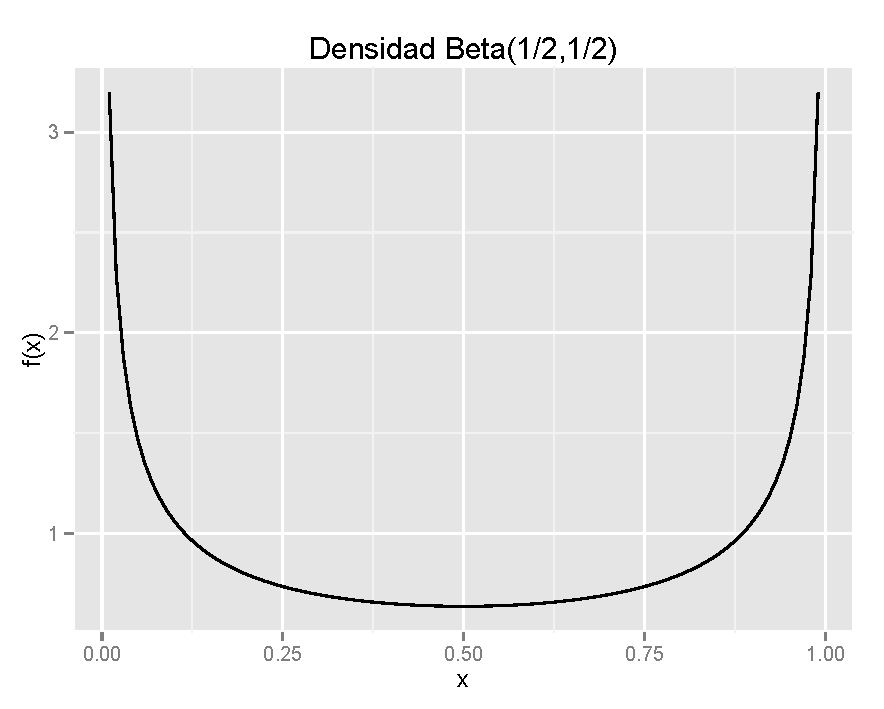
\includegraphics[scale=0.5]{Beta_no_inf.pdf}
    \caption{\emph{Distribuci\'on previa no informativa de Jeffreys para el par\'ametro de una distribuci\'on Bernoulli}}
    \end{figure}
    
    \begin{Res}
    La distribuci\'on predictiva previa para una observaci\'on $y$ est\'a dada por
    \begin{equation}\label{Predi_previa_bernou}
    p(Y)=\frac{Beta(y+\alpha,\beta-y+1)}{Beta(\alpha,\beta)}I_{\{0,1\}}(y),
    \end{equation}
    y define una aut\'entica funci\'on de densidad de probabilidad continua.
    \end{Res}
    
    \begin{proof}
    De la definici\'on de funci\'on de distribuci\'on predictiva se tiene que
    \begin{align*}
    p(Y)&=\int p(Y \mid \theta)p(\theta \mid \alpha,\beta)\ d\theta\\
    &=\int_0^1 \theta^y(1-\theta)^{1-y}I_{\{0,1\}}(y)\frac{1}{Beta(\alpha,\beta)}\theta^{\alpha-1}(1-\theta)^{\beta-1}\ d\theta\\
    &=\frac{Beta(y+\alpha,\beta-y+1)}{Beta(\alpha,\beta)}I_{\{0,1\}}(y)
    \int_0^1\frac{\theta^{y+\alpha-1}(1-\theta)^{\beta-y+1-1}}{Beta(y+\alpha,\beta-y+1)}\ d\theta\\
    &=\frac{Beta(y+\alpha,\beta-y+1)}{Beta(\alpha,\beta)}I_{\{0,1\}}(y)
    \end{align*}
    
    N\'otese que en la anterior demostraci\'on, la integral al lado derecho de la tercera igualdad es igual a la unidad, puesto que la expresi\'on matem\'atica dentro de la integral corresponde a la funci\'on de densidad de una variable aleatoria con distribucion $Beta$, que tiene rango en el intervalo $(0,1)$. Por otro lado se deben verificar las dos condiciones de funci\'on de densidad. Es decir
    \begin{enumerate}
    \item $p(Y)>0 ~(\forall y\in Y)$. Esta condici\'on se tiene trivialmente puesto que la funci\'on matem\'atica Beta siempre toma valores positivos.
    \item $\int p(y)\ dx=1$. En este caso, esta funci\'on es discreta definida en el conjunto $\{0,1\}$. Por lo tanto esta condici\'on es equivalente a
    \begin{equation*}
    \sum_{y\in{\{0,1\}}}P(Y=y)=\sum_{y\in{\{0,1\}}}\frac{Beta(y+\alpha,\beta-y+1)}{Beta(\alpha,\beta)}=1
    \end{equation*}
    Lo cual se verifica f\'acilmente teniendo en cuenta las propiedades de la funci\'on matem\'atica Beta y de la funci\'on matem\'atica Gamma.
    \end{enumerate}
    \end{proof}
    
    La distribuci\'on predictiva dada en \ref{Predi_previa_bernou} est\'a basada \'unicamente en la distribuci\'on previa del par\'ametro $\theta$, una vez observada la variable $Y$ se puede pensar en actualizar la distribuci\'on predictiva basando en la distribuci\'on posterior del par\'ametro, esta distribuci\'on se da en el siguiente resultado.
    
    \begin{Res}
    Despu\'es de la recolecci\'on de los datos, la distribuci\'on predictiva posterior para una nueva observaci\'on $\tilde{y}$ est\'a dada por
    \begin{equation}
    p(\tilde{y} \mid Y)=\frac{Beta(\tilde{y}+y+\alpha,\beta-\tilde{y}-y+2)}{Beta(y+\alpha,\beta-y+1)}I_{\{0,1\}}(\tilde{y}),
    \end{equation}
    \end{Res}
    
    \begin{proof}
    De la definici\'on de funci\'on de distribuci\'on predictiva se tiene que
    \begin{align*}
    p(\tilde{y} \mid Y)&=\int p(\tilde{y} \mid \theta)p(\theta \mid Y)\ d\theta\\
    &=\int_0^1\theta^{\tilde{y}}(1-\theta)^{1-\tilde{y}}I_{\{0,1\}}(\tilde{y})
    \frac{\theta^{y+\alpha-1}(1-\theta)^{\beta-y+1-1}}{Beta(y+\alpha,\beta-y+1)}\ d\theta\\
    &=\frac{Beta(\tilde{y}+y+\alpha,\beta-\tilde{y}-y+2)}{Beta(y+\alpha,\beta-y+1)}I_{\{0,1\}}(\tilde{y})\\
    &\hspace{2cm}\times \int_0^1\frac{\theta^{\tilde{y}+y+\alpha-1}(1-\theta)^{\beta-\tilde{y}-y+2-1}}
    {Beta(\tilde{y}+y+\alpha,\beta-\tilde{y}-y+2)}\ d\theta\\
    &=\frac{Beta(\tilde{y}+y+\alpha,\beta-\tilde{y}-y+2)}{Beta(y+\alpha,\beta-y+1)}I_{\{0,1\}}(\tilde{y})
    \end{align*}
    \end{proof}
    
    Ahora, en la pr\'actica rara vez se observa la realizaci\'on de una \'unica variable aleatoria Bernoulli $Y$, sino una muestra de variables aleatorias $Y_1$, $\cdots$, $Y_n$. En este caso, la distribuci\'on posterior del par\'ametro $\theta$ est\'a dada en el siguiente resultado.
    
    \begin{Res}
    Cuando se tiene una muestra aleatoria $Y_1,\ldots,Y_n$ de variables con distribuci\'on Bernoulli de par\'ametro $\theta$, entonces la distribuci\'on posterior del par\'ametro de inter\'es es
    \begin{equation*}
    \theta \mid Y_1,\ldots,Y_n \sim Beta\left(\sum_{i=1}^ny_i+\alpha,\beta-\sum_{i=1}^ny_i+n\right)
    \end{equation*}
    \end{Res}
    
    La demostraci\'on se deja como ejercicio.
    
    \begin{Eje}
    Es com\'un en muchos pa\'ises del mundo que se presenten encuestas de opini\'on electoral unas semanas antes de las elecciones presidenciales. Dentro de este tipo de encuestas se acostumbra a indagar acerca del favoritismo de los candidatos involucrados en la contienda electoral. Suponga que un candidato presidencial llamado Jos\'e P\'erez est\'a interesado en conocer su intenci\'on de voto previa a las elecciones. Para esto, \'el contrata a una firma encuestadora para la realizaci\'on de un muestreo probabil\'istico entre la poblaci\'on votante. El resultado de este estudio puede hacer cambiar o afirmar las estrategias publicitarias y la redefinici\'on de la campa\~na electoral. La firma encuestadora decide implementar una estrategia de muestreo con un tama\~no de muestra de doce mil personas. A cada respondiente se le realiza la siguiente pregunta: \textbf{Si las elecciones presidenciales fueran ma\~nana. ?Usted votar\'ia por el candidato Jos\'e P\'erez?}
    
    Las respuestas a esta pregunta son realizaciones de una muestra aleatoria de doce mil variables con densidad Bernoulli. Los resultados del estudio arrojan que 6360 personas de las personas entrevistadas, es decir un 53 por ciento, votar\'ian por el suscrito candidato. T\'ecnicamente se debe analizar esta cifra puesto que las implicaciones de ganar en una primera vuelta son grandes en el sentido econ\'omico, log\'istico y administrativo. Claramente, el dato 53 por ciento asegura una ventaja dentro de la muestra de doce mil personas. Sin embargo, es necesario realizar un estudio m\'as profundo acerca de la caracterizaci\'on estructural de la intenci\'on de voto del candidato en la poblaci\'on de todos los votantes.
    
    Con base en lo anteriormente expuesto, se decide utilizar la inferencia bayesiana puesto que existe informaci\'on previa de un estudio anterior, contratado por el mismo candidato unos meses atr\'as en donde se entrevistaron a mil personas, con un favoritismo que estaba alrededor del 35 por ciento. Esta situaci\'on conlleva a la utilizaci\'on de la metodolog\'ia bayesiana que incorpora la informaci\'on pasada acerca del mismo fen\'omeno.
    
    El estad\'istico de la firma encuestadora decide utilizar una distribuci\'on previa\footnote{Como se ver\'a m\'as adelante, es conveniente definir los par\'ametros de la distribuci\'on previa como $\alpha$ igual al n\'umero de votantes a favor y $\beta$ igual al n\'umero de votantes en contra.} $Beta(\alpha=350, \beta=650)$. Utilizando el resultado 2.1.4, se contempla que la distribuci\'on posterior del par\'ametro de inter\'es, que representa la probabilidad de \'exito en las elecciones presidenciales, es $Beta(6360+350, 650-6360+12000)=Beta(6710, 6290)$. Por lo tanto, utilizando la distribuci\'on posterior, se estima que la intenci\'on de voto por el candidato es de $\frac{6710}{6710+6290}=\frac{6710}{13000}=0.516$ y este valor equivale a la media de la distribuci\'on posterior. Este mismo an\'alisis puede ejecutarse en \texttt{JAGS}, mediante el uso del siguiente c\'odigo computacional
    
    Sin embargo, si no se tuviese informaci\'on previa como la suministrada por el estudio de meses anteriores, el an\'alisis bayesiano sugerir\'ia trabajar con una distribuci\'on previa no informativa, que en este caso, corresponder\'ia a una $Beta(\alpha=0.5, \beta=0.5)$. siguiendo el mismo an\'alisis, se tiene que la distribuci\'on posterior es $Beta(6360.5, 5640.5)$. Finalmente, se estimar\'ia que la intenci\'on de voto por el candidato es de $\frac{6350.5}{12001}=0.529$. Las figuras \ref{BernoEj1} y \ref{BernoEj2} muestran el comportamiento de las distribuciones previas y posteriores en ambos escenarios. N\'otese que la distribuci\'on no informativa influye muy poco en el comportamiento de la distribuci\'on posterior.
    
    \begin{figure}[!h]
    \centering
    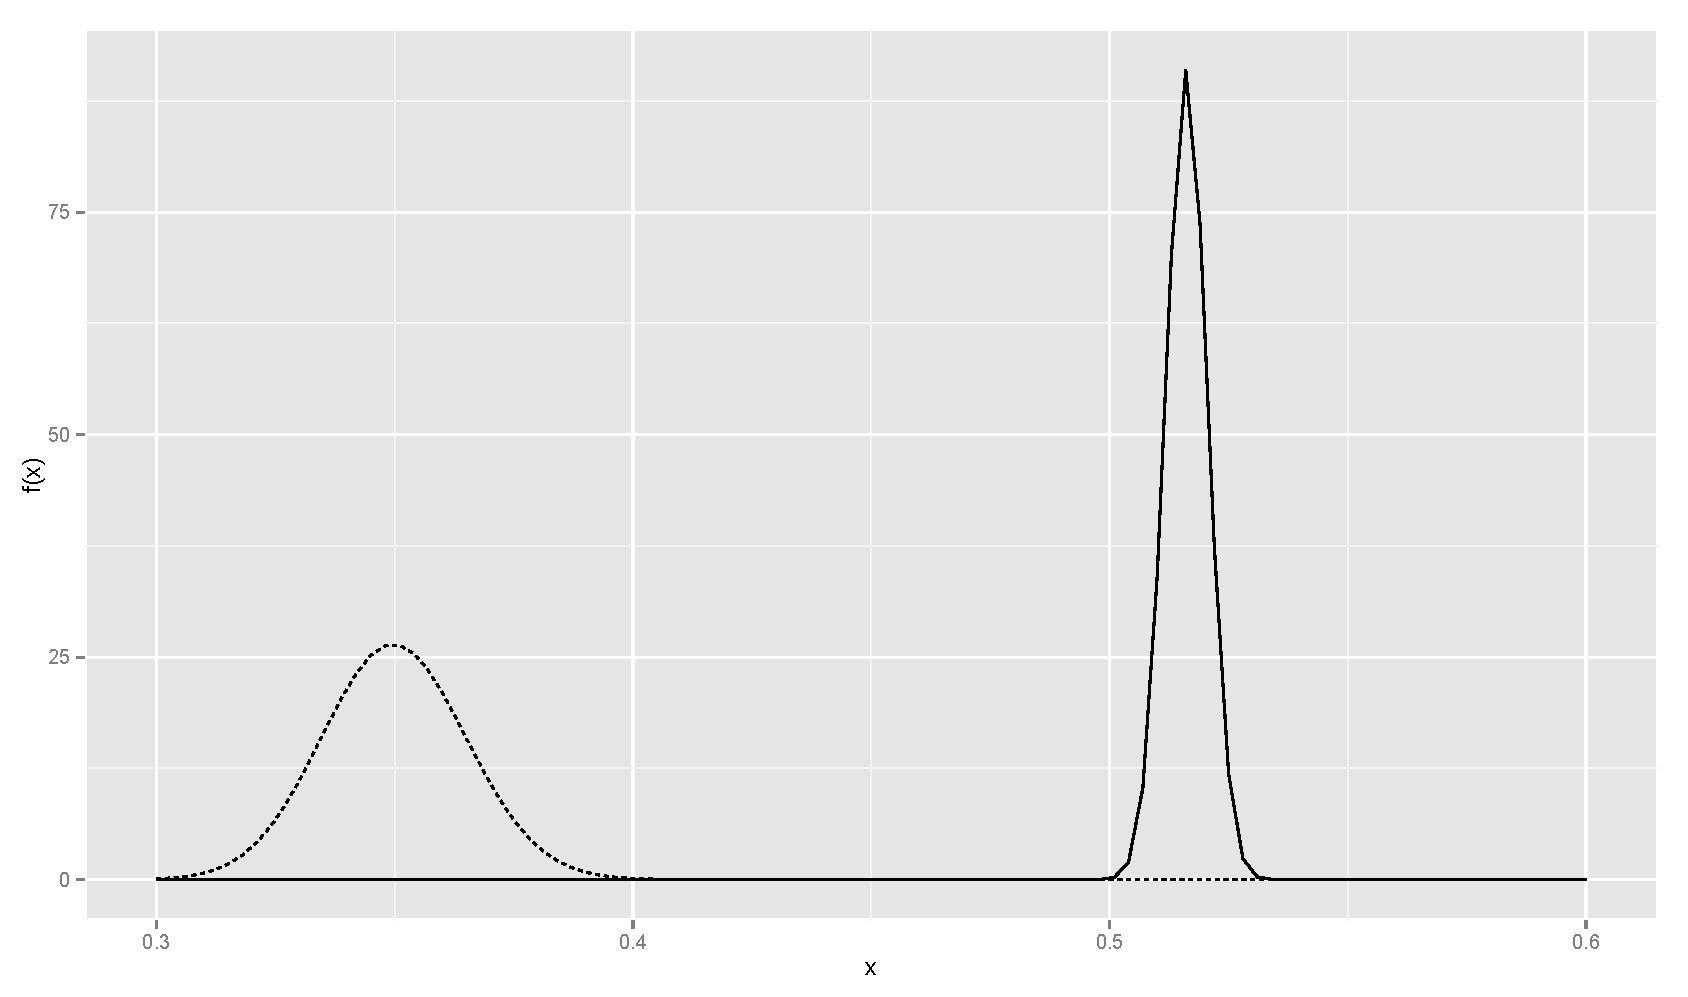
\includegraphics[scale=0.28]{BernoEj1.pdf}
    \caption{\emph{Distribuci\'on previa informativa (l\'inea punteada) y distribuci\'on posterior (l\'inea s\'olida) para el ejemplo de las encuestas electorales.}}
    \label{BernoEj1}
    \end{figure}
    
    \begin{figure}[!h]
    \centering
    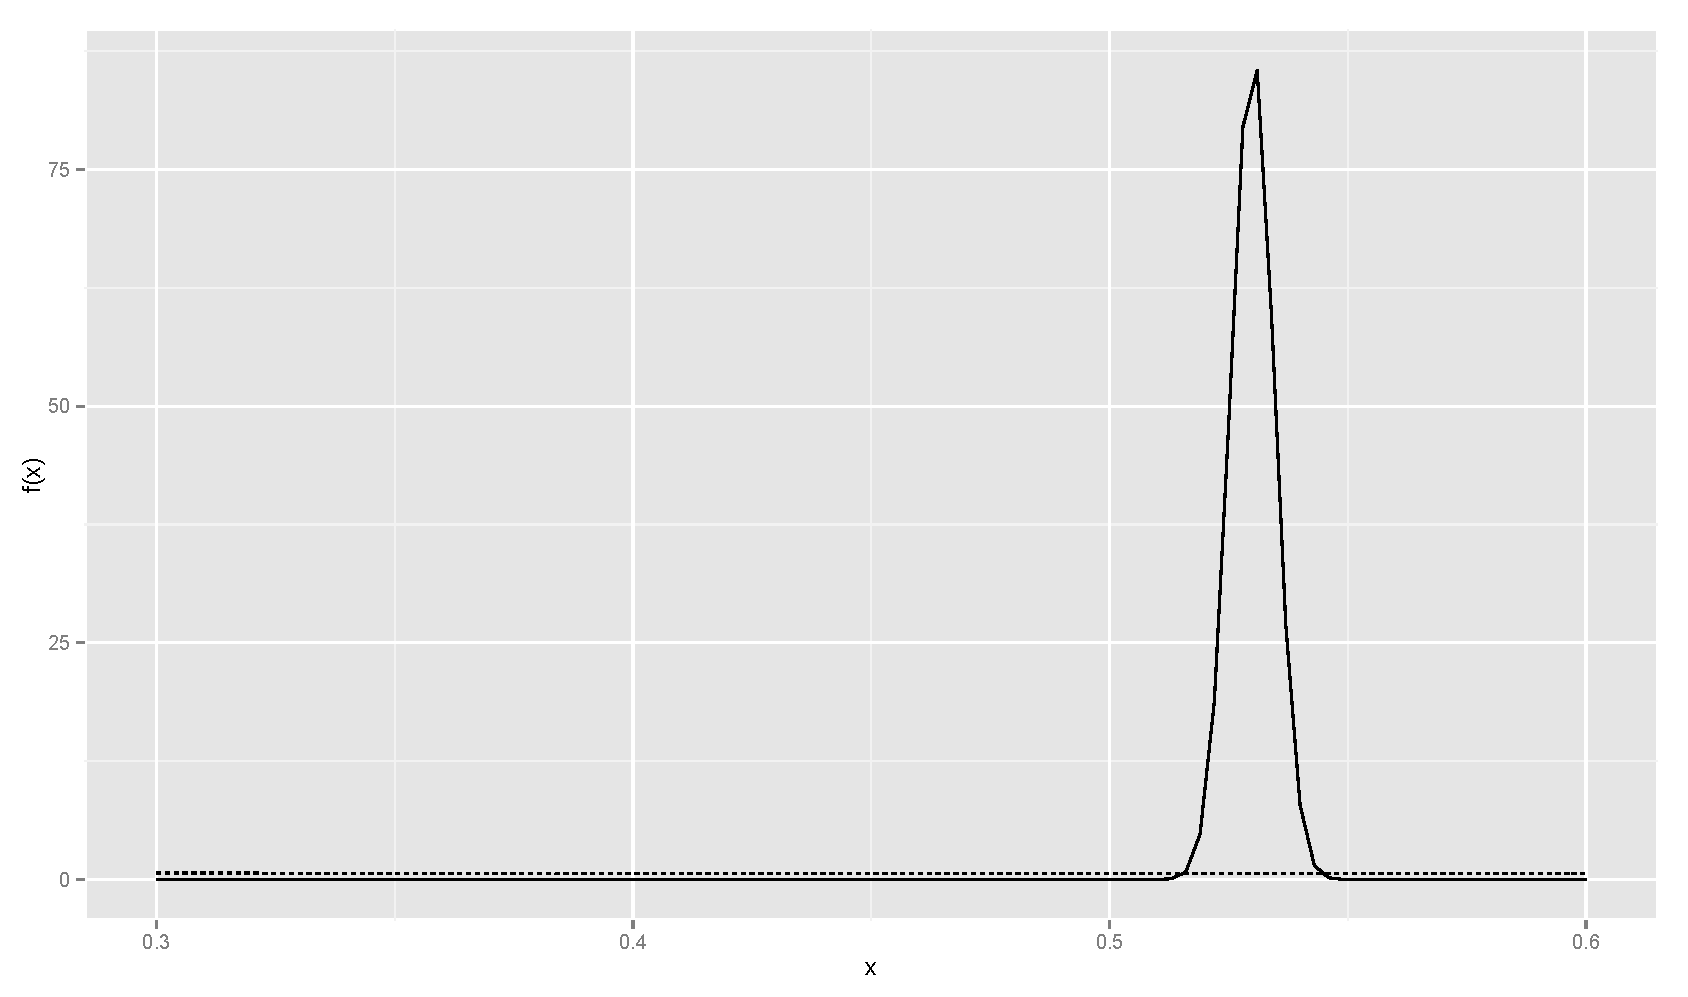
\includegraphics[scale=0.28]{BernoEj2.pdf}
    \caption{\emph{Distribuci\'on previa no informativa (l\'inea punteada) y distribuci\'on posterior (l\'inea s\'olida) para el ejemplo de las encuestas electorales.}}
    \label{BernoEj2}
    \end{figure}
    
    Utilizando el siguiente c\'odigo en R, es posible conocer los intervalos de credibilidad para las dos distribuciones posteriores. Es posible concluir que en ambos escenarios, el candidato aventaja significativamente a sus contrincantes y, salvo alg\'un cambio dr\'astico en el comportamiento del electorado, ganar\'a las elecciones. Lo anterior se deduce puesto que el intervalo de credibilidad al 95\% no contiene ning\'un valor menor a 0.5
    
\begin{knitrout}
\definecolor{shadecolor}{rgb}{0.933, 0.933, 0.933}\color{fgcolor}\begin{kframe}
\begin{alltt}
\hlkwd{qbeta}\hlstd{(}\hlkwd{c}\hlstd{(}\hlnum{0.025}\hlstd{,} \hlnum{0.975}\hlstd{),}\hlnum{6710}\hlstd{,}\hlnum{6290}\hlstd{)}
\end{alltt}
\begin{verbatim}
## [1] 0.5076 0.5247
\end{verbatim}
\begin{alltt}
\hlkwd{qbeta}\hlstd{(}\hlkwd{c}\hlstd{(}\hlnum{0.025}\hlstd{,}\hlnum{0.975}\hlstd{),}\hlnum{6350.5}\hlstd{,}\hlnum{5640.5}\hlstd{)}
\end{alltt}
\begin{verbatim}
## [1] 0.5207 0.5385
\end{verbatim}
\end{kframe}
\end{knitrout}
    
\begin{verbatim}
> qbeta(c(0.025, 0.975),6710,6290)
[1] 0.5075614 0.5247415
>     qbeta(c(0.025,0.975),6350.5,5640.5)
[1] 0.5206678 0.5385340
\end{verbatim}
    Por otro lado, el siguiente c\'odigo en JAGS permite obtener el mismo tipo de inferencia creando tres cadenas de Markov cuya distribuci\'on de probabilidad coincide con la distribuci\'on posterior del ejemplo.
    
    \begin{mdframed}
    \begin{verbatim}
    #datos
    y <- c(1, 0, 1,..., 0)
    n <-length(y)
    
    #modelo jags Bernoulli
    Bern.model <-function() {
    for(i in 1:n)
    {
    y[i]~dbern(theta)
    }
    theta~dbeta(350, 650)#informaci\'on previa 
    }
    
    bern.data <- list("y","n")
    bern.param <- c("theta")
    bern.inits <- function(){list("theta"=c(0.5))}
    set.seed(123)
    
    bern.fit <- jags(data=bern.data, inits=bern.inits, bern.param, 
    n.chains=3, n.iter=10000, n.burnin=1000,
    n.thin=10, model.file=bern.model)
    
    print(bern.fit)
    \end{verbatim}
    \end{mdframed}
    \end{Eje}
    
    \section{Modelo Binomial}
    
    Cuando se dispone de una muestra aleatoria de variables con distribuci\'on Bernoulli $Y_1,\ldots,Y_n$, la inferencia bayesiana se puede llevar a cabo usando la distribuci\'on Binomial, puesto que es bien sabido que la suma de variables aleatorias Bernoulli
    \begin{equation*}
    S=\sum_{i=1}^nY_i
    \end{equation*}
    sigue una distribuci\'on Binomial. Es decir:
    \begin{equation}
    p(S \mid \theta)=\binom{n}{s}\theta^s(1-\theta)^{n-s}I_{\{0,1,\ldots,n\}}(s),
    \end{equation}
    
    N\'otese que la distribuci\'on binomial es un caso general para la distribuci\'on Bernoulli, cuando $n=1$. Entonces, as\'i como en la distribuci\'on Bernoulli, el par\'ametro $\theta$ est\'a restringido al espacio $\Theta=[0,1]$. Luego, es admisible proponer que $\theta$ siga una distribuci\'on Beta. Por tanto la distribuci\'on previa del par\'ametro $\theta$ est\'a dada por la expresi\'on (2.1.2). Bajo este marco de referencia se tienen los siguientes resultados
    
    \begin{Res}
    La distribuci\'on posterior del par\'ametro $\theta$ sigue una distribuci\'on
    \begin{equation*}
    \theta \mid S \sim Beta(s+\alpha,\beta-s+n)
    \end{equation*}
    \end{Res}
    
    \begin{proof}
    \begin{align*}
    p(\theta \mid S)&\propto p(S \mid \theta)p(\theta \mid \alpha,\beta)\\
    &=\frac{\binom{n}{s}I_{\{0,1,\ldots,n\}}(s)}{Beta(\alpha,\beta)}
    \theta^s\theta^{\alpha-1} (1-\theta)^{\beta-1}(1-\theta)^{n-s}I_{[0,1]}(\theta)\\
    &\propto \theta^{s+\alpha-1} (1-\theta)^{\beta-s+n-1}I_{[0,1]}(\theta)
    \end{align*}
    Por lo tanto, factorizando convenientemente, se llega a una expresi\'on id\'entica a la funci\'on de distribuci\'on de una variable aleatoria con distribuci\'on $Beta(s+\alpha,\beta-s+n)$.
    
    \end{proof}
    
    Del resultado anterior podemos ver que el estimador bayesiano de $\theta$ est\'a dada por la media de la distribuci\'on posterior, dada por
    \begin{equation}\label{esti_beta}
    \hat{\theta}_{B}=\frac{s+\alpha}{n+\alpha+\beta}
    \end{equation}
    
    En la pr\'actica, se acostumbra a escoger los hiperpar\'ametros $\alpha$ y $\beta$ de tal forma que correspondan al n\'umero de \'exitos y fracasos obtenidos en los datos previa, respectivamente. De esta forma, $\hat{\theta}_{P}=\alpha/(\alpha+\beta)$ corresponde a la estimaci\'on previa del par\'ametro $\theta$. Por otro lado, el estimador cl\'asico de $\theta$ est\'a dado por $\hat{\theta}_{C}=s/n$. Entonces es posible notar que el estimador bayesiano de $\theta$ en (\ref{esti_beta}) de alguna forma combina el estimador cl\'asico y el estimador previa. M\'as a\'un, se puede ver que $\hat{\theta}_{B}$ se puede escribir como un promedio ponderado entre la estimaci\'on cl\'asica y la estimaci\'on previa. Puesto que
    \begin{align*}
    \hat{\theta}_{B}=\frac{s+\alpha}{n+\alpha+\beta}&=\frac{s}{n+\alpha+\beta}+\frac{\alpha}{n+\alpha+\beta}\\
    &=\frac{n}{n+\alpha+\beta}\frac{s}{n}+\frac{\alpha+\beta}{n+\alpha+\beta}\frac{\alpha}{\alpha+\beta}\\
    &=\frac{n}{n+\alpha+\beta}\hat{\theta}_{C}+\frac{\alpha+\beta}{n+\alpha+\beta}\hat{\theta}_{P}
    \end{align*}
    
    De esta forma, queda en evidencia que la estimaci\'on bayesiana de $\theta$ siempre ser\'a un valor intermedio entre la estimaci\'on cl\'asica y la estimaci\'on previa. La gr\'afica \ref{beta3} da una ilustraci\'on acerca de la anterior afirmaci\'on, en donde se puede observar que para una distribuci\'on previa concentrada en $2/7$ y una funci\'on de verosimilitud\footnote{La funci\'on de verosimilitud es una funci\'on del par\'ametro y s\'olo se puede graficar una vez se hayan observado las realizaciones de la variable aleatoria.} con m\'aximo en $8/10$, se tiene una distribuci\'on posterior centrada en $10/17$; es decir, la estimaci\'on bayesiana se encuentra situada entre la estimaci\'on previa y la estimaci\'on cl\'asica.
    
    \begin{figure}[!h]
    \centering
    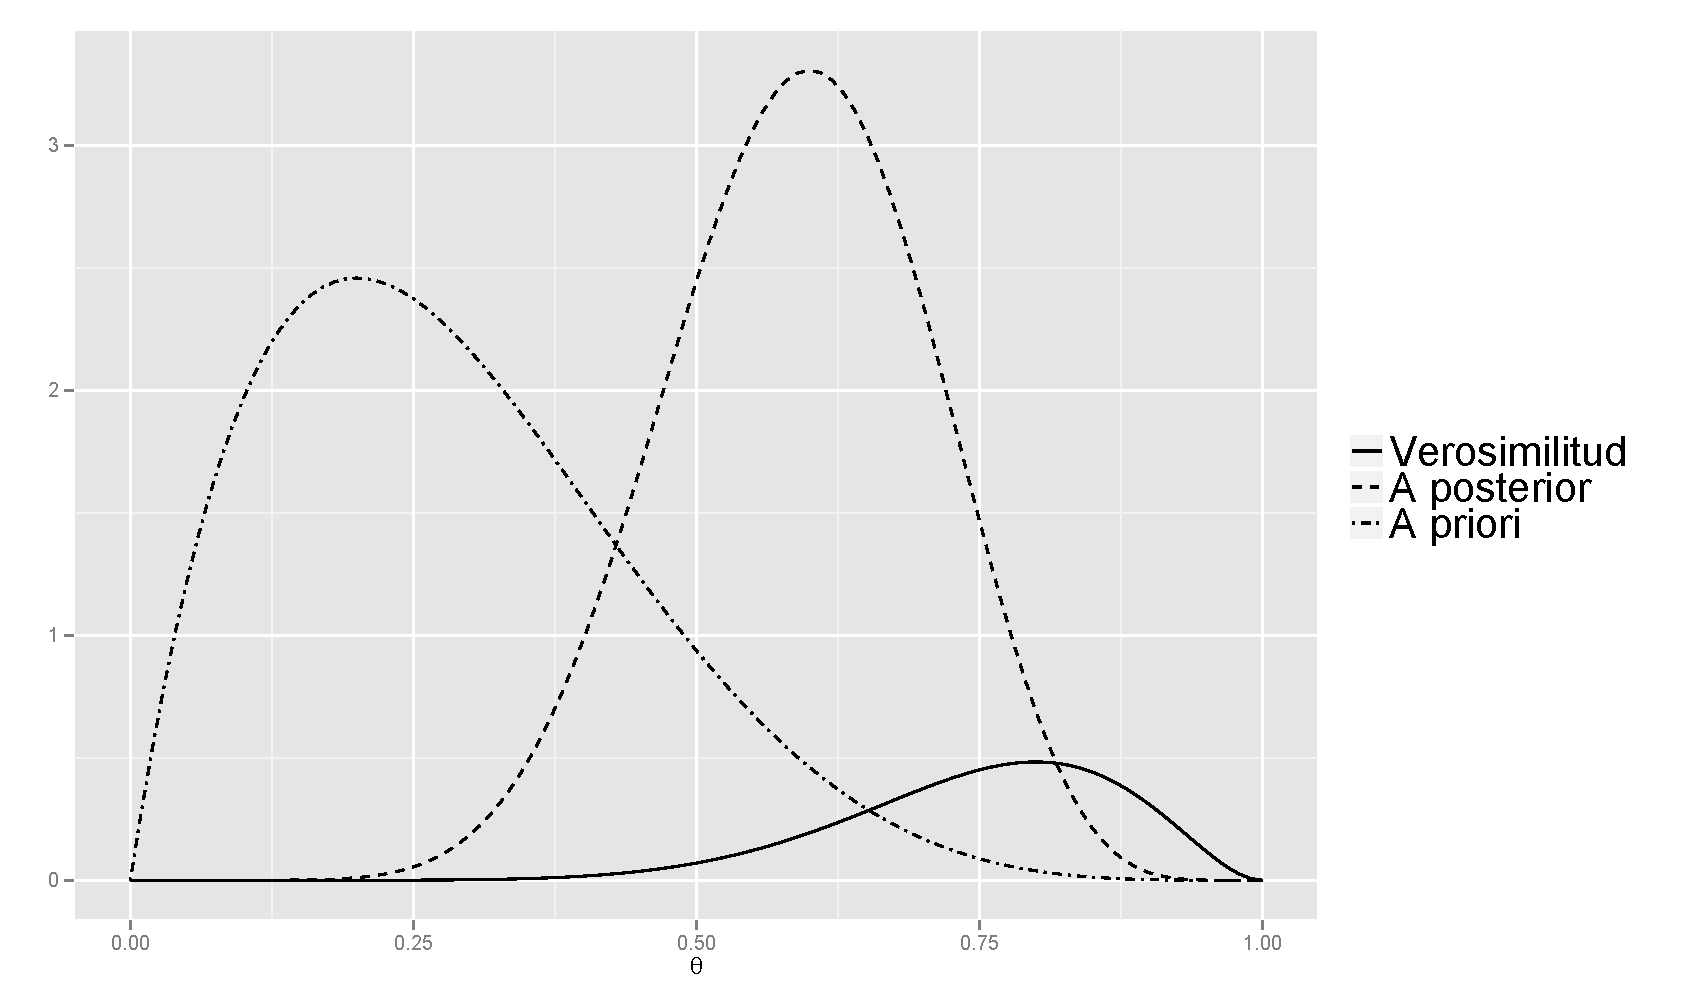
\includegraphics[scale=0.4]{Beta_tres.pdf}
    \caption{\emph{Funci\'on de verosimilitud, funci\'on de densidad previa y posterior para $\alpha=2$, $\beta=5$, $s=8$ y $n=10$.}}
    \label{beta3}
    \end{figure}
    
    Por otro lado, entre m\'as grande sea el tama\~no muestral $n$, m\'as cercano estar\'a $\hat{\theta}_{B}$ de $\hat{\theta}_{C}$ o equivalentemente la funci\'on de densidad posterior de $\theta$ estar\'a m\'as concentrada en $s/n$; mientras que entre mayor n\'umero de datos tenga la muestra de la distribuci\'on previa ($\alpha+\beta$=n\'umero de datos), m\'as cercano estar\'a $\hat{\theta}_{B}$ de $\hat{\theta}_{P}$ y la densidad posterior de $\theta$ estar\'a m\'as concentrada en $\alpha/(\alpha+\beta)$.
    
    Para ilustrar lo anterior, suponga que la distribuci\'on previa de $\theta$ est\'a dada con $\alpha=\beta=5$, es decir la estimacion previa es 0.5, y suponga adem\'as que la estimaci\'on cl\'asica es 0.33, pero el tama\~no muestral $n$ incrementa manteniendo constante la estimacion cl\'asica. En la figura \ref{betan} se muestra la estimaci\'on posterior de $\theta$, es evidente que a medida que el tama\~no muestral $n$ aumenta, la estimaci\'on posterior se acerca m\'as a la estimaci\'on cl\'asica.
    
    \begin{figure}[!h]
    \centering
    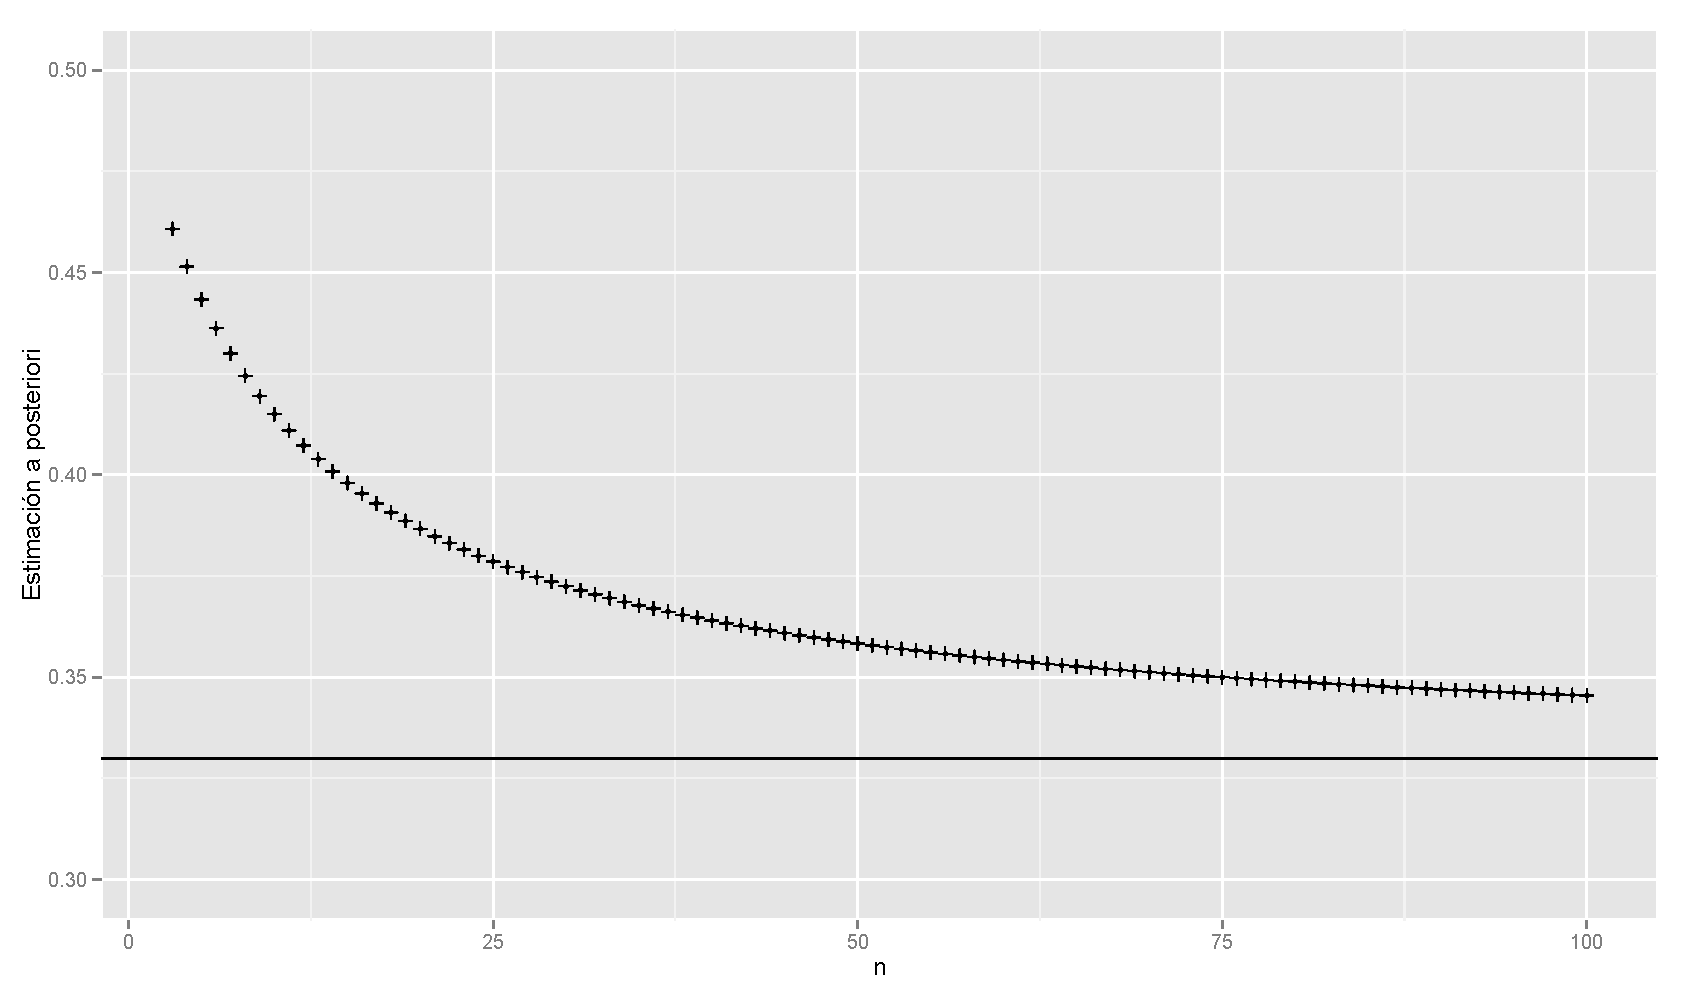
\includegraphics[scale=0.35]{Beta_n_aumen.pdf}
    \caption{\emph{Estimaci\'on posterior de $\theta$ para diferentes valores de $n$ y $s$ con $\alpha=\beta=5$.}}
    \label{betan}
    \end{figure}
    
    Anteriormente, se coment\'o que se acostumbra a escoger los par\'ametros $\alpha$ y $\beta$ que correspondan al n\'umero de \'exitos y fracasos en la informaci\'on previa, sin embargo, la informaci\'on previa puede no presentarse de esta forma. Por ejemplo, en algunas situaciones, la informaci\'on previa puede proveer el valor de $\theta$, es decir, el valor de $\hat{\theta}_P$, y el valor de la desviaci\'on est\'andar de la estimaci\'on (com\'unmente conocido como el error est\'andar). Por ejemplo, suponga que $\hat{\theta}_P=0.5$ con un error est\'andar de 0.1, entonces podemos encontrar los valores de $\alpha$ y $\beta$ de las expresiones $\frac{\alpha}{\alpha+\beta}=0.5$ y $\sqrt{\frac{\alpha\beta}{(\alpha+\beta)^2(\alpha+\beta+1)}}=0.1$, de donde se tiene que $\alpha=12$ y $\beta=12$, y la distribuci\'on a priori correspondiente $Beta(12,12)$ tiene una esperanza de 0.05 y una desviaci\'on est\'andar de 0.1. Se puede ver que entre mayor sea la desviaci\'on est\'andar, menores resultan los valores de $\alpha$ y $\beta$, que conducen a una distribuci\'on previa menos informativa.
    
    Ahora, se vio anteriomente que la distribuci\'on previa no informativa de Jeffreys corresponde a la distribuci\'on $Beta(1/2,1/2)$, la cual conduce a la distribuci\'on posterior $Beta(s+1/2,n-s+1/2)$, que a su vez nos lleva al estimador 
    \begin{equation}
    \label{Esti_theta_Jeffreys}
    \hat{\theta}_B=\frac{s+1/2}{n+1}
    \end{equation}
    
    La anterior expresi\'on es comparable con el estimador cl\'asico $\hat{\theta_C}=\frac{s}{n}$, en el sentido de que los dos son aplicables cuando no se dispone de ninguna informaci\'on previa. Podemos observar que aparte del alto grado de similitud que tienen los dos estimadores, es preferible usar el estimador (\ref{Esti_theta_Jeffreys}) en situaciones donde el valor te\'orico de $\theta$ es muy peque\~no, y como consecuencia en la muestra $s=0$, por ejemplo, cuando $\theta$ representa el porcentaje de personas que esten infectados con alg\'un virus poco com\'un. En estos casos, el estimador cl\'asico $\hat{\theta}_C=0$ sugiriendo que ning\'un porcentaje de la poblaci\'on est\'a infectado, conclusi\'on que puede ser err\'onea; por otro lado, el estimador bayesiano $\hat{\theta}_B=\frac{0.5}{n+1}$, el cual tiende a ser un porcentaje muy peque\~no a medida que aumente el tama\~no muestral $n$, pero nunca llega a dar el valor 0 como la estimaci\'on de $\theta$.
    
    En el siguiente resultado, se encuentra la distribuci\'on predictiva previa para una variable binomial $S$.
    
    \begin{Res}
    La distribuci\'on predictiva previa para la observaci\'on particular de la suma de variables aleatorias Bernoulli, $s$, est\'a dada por una distribuci\'on Beta-Binomial dada por
    \begin{equation}
    p(S)=\binom{n}{s}\frac{Beta(s+\alpha,\beta-s+n)}{Beta(\alpha,\beta)}I_{\{0,1,\ldots,n\}}(s).
    \end{equation}
    \end{Res}
    
    \begin{proof}
    De la definici\'on de funci\'on de distribuci\'on predictiva previa se tiene que
    \begin{align*}
    p(S)&=\int p(S \mid \theta)p(\theta \mid \alpha,\beta)\ d\theta\\
    &=\int_0^1\binom{n}{s}\theta^s(1-\theta)^{n-s}I_{\{0,1,\ldots,n\}}(s)
    \frac{1}{Beta(\alpha,\beta)}\theta^{\alpha-1}(1-\theta)^{\beta-1}\ d\theta\\
    &=\binom{n}{s}\frac{Beta(s+\alpha,\beta-s+n)}{Beta(\alpha,\beta)}I_{\{0,1,\ldots,n\}}(s)\\
    &\hspace{2cm}\times\int_0^1\frac{\theta^{s+\alpha-1}(1-\theta)^{\beta-s+n-1}}{Beta(s+\alpha,\beta-s+n)}\ d\theta\\
    &=\binom{n}{s}\frac{Beta(s+\alpha,\beta-s+n)}{Beta(\alpha,\beta)}I_{\{0,1,\ldots,n\}}(s)
    \end{align*}
    \end{proof}
    
    
    Una vez observados los valores muestrales, podemos encontrar la distribuci\'on predictiva posterior para una nueva variable binomial $\tilde{S}$ en una muestra de tama\~no $\tilde{n}$. Esta distribuci\'on se encuentra en el siguiente resultado.
    \begin{Res}
    \label{ResPredBinom}
    Despu\'es de la recolecci\'on de los datos $y_1$, $\cdots$, $y_n$, la distribuci\'on predictiva posterior para una nueva variable $\tilde{S}$ en una muestra del tama\~no $\tilde{n}$ est\'a dada por
    \begin{equation}\label{Binom_predict}
    p(\tilde{s} \mid S)=\binom{\tilde{n}}{\tilde{s}}\frac{Beta(\tilde{s}+s+\alpha,\beta-\tilde{s}-s+n+\tilde{n})}{Beta(s+\alpha,\beta-s+n)}I_{\{0,1,\ldots,\tilde{n}\}}(\tilde{s}),
    \end{equation}
    \end{Res}
    
    \begin{proof}
    De la definici\'on de funci\'on de distribuci\'on predictiva se tiene que
    \begin{align*}
    p(\tilde{s} \mid S)&=\int p(\tilde{s} \mid \theta)p(\theta \mid S)\ d\theta\\
    &=\int_0^1 \binom{\tilde{n}}{\tilde{s}} \theta^{\tilde{s}}(1-\theta)^{\tilde{n}-\tilde{s}}I_{\{0,1,\ldots,\tilde{n}\}}(\tilde{s})
    \frac{\theta^{s+\alpha-1}(1-\theta)^{\beta-s+n-1}}{Beta(s+\alpha,\beta-s+n)}\ d\theta\\
    &=\binom{\tilde{n}}{\tilde{s}}\frac{Beta(\tilde{s}+s+\alpha,\beta-\tilde{s}-s+n+\tilde{n})}{Beta(s+\alpha,\beta-s+n)}I_{\{0,1,\ldots,\tilde{n}\}}(\tilde{s})\\
    & \hspace{2cm}\times
    \int_0^1\frac{\theta^{\tilde{s}+s+\alpha-1}(1-\theta)^{\beta-\tilde{s}-s+n+\tilde{n}-1}}
    {Beta(\tilde{s}+s+\alpha,\beta-\tilde{s}-s+n+\tilde{n})}\ d\theta\\
    &=\binom{\tilde{n}}{\tilde{s}}\frac{Beta(\tilde{s}+s+\alpha,\beta-\tilde{s}-s+n+\tilde{n})}{Beta(s+\alpha,\beta-s+n)}I_{\{0,1,\ldots,\tilde{n}\}}(\tilde{s})
    \end{align*}
    \end{proof}
    
    En la anterior distribuci\'on predictiva, se necesita calcular funciones Beta. Cuando los tama\~nos muestrales $n$, $\tilde{n}$ y/o los par\'ametros de la distribuci\'on previa $\alpha$ y $\beta$ son muy grandes, puede presentar problemas num\'ericos al momento de calcular directamente estas funciones Beta. Por ejemplo, supongamos que $n=1000$, $s=650$, $\alpha=200$, $\beta=300$ y $\tilde{n}=800$, de esta forma, los posibles valores para $\tilde{s}$ son $0,1,\cdots,800$, y se tiene que la probabilidad de que $\tilde{s}$ tome el valor 500 est\'a dada por
    \begin{equation}\label{Eje_binom}
    Pr(\tilde{s}=500|S)=\binom{800}{500}\frac{Beta(1350,950)}{Beta(850,650)}
    \end{equation}
    
    y desafortunadamente, en \textsf{R}, se presenta error al intentar ejecutar \texttt{beta(1350,950)} o \texttt{beta(850,650)}. Planteamos la siguiente soluci\'on num\'erica cuando se quiere calcular la funci\'on predictiva (\ref{Binom_predict}) en muestras grandes. El problema central es el c\'omputo de $\frac{Beta(a,b)}{Beta(c,d)}$ con $a\geq c$ y $b\geq d$, valores enteros. Podemos ver que
    
    \begin{align*}
    &\ \ \ \ \frac{Beta(a,b)}{Beta(c,d)}\\
    &=\frac{(a-1)!(b-1)!(c+d-1)!}{(c-1)!(d-1)!(a+b-1)!}\\
    &=\frac{(a-1)(a-2)\cdots(a-(a-c))(b-1)(b-2)\cdots(b-(b-d))}{(a+b-1)(a+b-2)\cdots(a+b-(a+b-c-d))}\\
    &=\frac{a^{a-c}(1-\frac{1}{a})(1-\frac{2}{a})\cdots(1-\frac{a-c}{a})b^{b-d}(1-\frac{1}{b})(1-\frac{2}{b})\cdots(1-\frac{b-d}{b})}{(a+b)^{a+b-c-d}(1-\frac{1}{a+b})(1-\frac{2}{a+b})\cdots(1-\frac{a+b-c-d}{a+b})}\\
    &=\underbrace{\left(\frac{a}{a+b}\right)^{a-c}}_{t1}\underbrace{\left(\frac{b}{a+b}\right)^{b-d}}_{t2}\underbrace{(1-\frac{1}{a})(1-\frac{2}{a})\cdots(1-\frac{a-c}{a})}_{t3}\\
    &\ \ \ \ \ \ \underbrace{(1-\frac{1}{b})(1-\frac{2}{b})\cdots(1-\frac{b-d}{b})}_{t4}\underbrace{(1-\frac{1}{a+b})(1-\frac{2}{a+b})\cdots(1-\frac{a+b-c-d}{a+b})}_{t5}
    \end{align*}
    
    Calculando separadamente los t\'erminos $t1$, $t2$, $t3$, $t4$ y $t5$ podemos calcular $\frac{Beta(a,b)}{Beta(c,d)}$ para valores grandes de $a$, $b$, $c$ y $d$. La siguiente funci\'on \verb"prob" calcula la densidad (\ref{Binom_predict}) para un valor particular de $\tilde{s}$ usando la anterior t\'ecnica.
    
\begin{knitrout}
\definecolor{shadecolor}{rgb}{0.933, 0.933, 0.933}\color{fgcolor}\begin{kframe}
\begin{alltt}
\hlstd{prob}\hlkwb{<-}\hlkwa{function}\hlstd{(}\hlkwc{s.mono}\hlstd{,}\hlkwc{n.mono}\hlstd{,}\hlkwc{s}\hlstd{,}\hlkwc{n}\hlstd{,}\hlkwc{alfa}\hlstd{,}\hlkwc{beta}\hlstd{)\{}
\hlstd{a}\hlkwb{<-}\hlstd{s.mono}\hlopt{+}\hlstd{s}\hlopt{+}\hlstd{alfa; b}\hlkwb{<-}\hlstd{n.mono}\hlopt{-}\hlstd{s.mono}\hlopt{+}\hlstd{n}\hlopt{-}\hlstd{s}\hlopt{+}\hlstd{beta}
\hlstd{c}\hlkwb{<-}\hlstd{s}\hlopt{+}\hlstd{alfa; d}\hlkwb{<-}\hlstd{n}\hlopt{-}\hlstd{s}\hlopt{+}\hlstd{beta}
\hlstd{t1}\hlkwb{<-}\hlstd{(a}\hlopt{/}\hlstd{(a}\hlopt{+}\hlstd{b))}\hlopt{^}\hlstd{(a}\hlopt{-}\hlstd{c); t2}\hlkwb{<-}\hlstd{(b}\hlopt{/}\hlstd{(a}\hlopt{+}\hlstd{b))}\hlopt{^}\hlstd{(b}\hlopt{-}\hlstd{d)}
\hlstd{t3}\hlkwb{<-}\hlkwd{prod}\hlstd{(}\hlnum{1}\hlopt{-}\hlkwd{c}\hlstd{(}\hlnum{1}\hlopt{:}\hlstd{(a}\hlopt{-}\hlstd{c))}\hlopt{/}\hlstd{a); t4}\hlkwb{<-}\hlkwd{prod}\hlstd{(}\hlnum{1}\hlopt{-}\hlkwd{c}\hlstd{(}\hlnum{1}\hlopt{:}\hlstd{(b}\hlopt{-}\hlstd{d))}\hlopt{/}\hlstd{b)}
\hlstd{t5}\hlkwb{<-}\hlkwd{prod}\hlstd{(}\hlnum{1}\hlopt{-}\hlkwd{c}\hlstd{(}\hlnum{1}\hlopt{:}\hlstd{(a}\hlopt{+}\hlstd{b}\hlopt{-}\hlstd{c}\hlopt{-}\hlstd{d))}\hlopt{/}\hlstd{(a}\hlopt{+}\hlstd{b))}
\hlkwa{if}\hlstd{(a}\hlopt{==}\hlstd{c)\{resul}\hlkwb{<-} \hlstd{t2}\hlopt{*}\hlstd{t4}\hlopt{/}\hlstd{t5\}}
\hlkwa{if}\hlstd{(b}\hlopt{==}\hlstd{d)\{resul}\hlkwb{<-}\hlstd{t1}\hlopt{*}\hlstd{t3}\hlopt{/}\hlstd{t5\}}
\hlkwa{if}\hlstd{(a}\hlopt{>}\hlstd{c}\hlopt{&}\hlstd{b}\hlopt{>}\hlstd{d)\{resul}\hlkwb{<-}\hlkwd{choose}\hlstd{(n.mono,s.mono)}\hlopt{*}\hlstd{t1}\hlopt{*}\hlstd{t2}\hlopt{*}\hlstd{t3}\hlopt{*}\hlstd{t4}\hlopt{/}\hlstd{t5\}}
\hlstd{resul \}}
\end{alltt}
\end{kframe}
\end{knitrout}
    
    
    Si queremos examinar la distribuci\'on predictiva para todos valores de la variable $\tilde{S}$, podemos usar los siguientes c\'odigos
\begin{knitrout}
\definecolor{shadecolor}{rgb}{0.933, 0.933, 0.933}\color{fgcolor}\begin{kframe}
\begin{alltt}
\hlstd{n}\hlkwb{<-}\hlnum{1000}\hlstd{; s}\hlkwb{<-}\hlnum{650}
\hlstd{alfa}\hlkwb{<-}\hlnum{200}\hlstd{; beta}\hlkwb{<-}\hlnum{300}
\hlstd{n.mono}\hlkwb{<-}\hlnum{800}
\hlstd{res}\hlkwb{<-}\hlkwd{rep}\hlstd{(}\hlnum{NA}\hlstd{,(}\hlnum{1}\hlopt{+}\hlstd{n.mono))}
\hlkwa{for}\hlstd{(i} \hlkwa{in} \hlnum{1}\hlopt{:}\hlkwd{length}\hlstd{(res))\{}
\hlstd{res[i]}\hlkwb{<-}\hlkwd{prob}\hlstd{(i}\hlopt{-}\hlnum{1}\hlstd{,n.mono,s,n,alfa,beta)}
\hlstd{\}}
\end{alltt}
\end{kframe}
\end{knitrout}
    
    y como resultado, \verb"res" contiene las 801 probabilidades asociadas a todos los posibles valores de $\tilde{s}$.
    
    Los resultados obtenidos con la anterior t\'ecnica es equivalente a lo obtenido usando la funci\'on \verb"lbeta" que computa el logaritmo natural de la funci\'on beta. As\'i, para calcular la probabilidad en (\ref{Eje_binom}), simplemente usamos el siguiente c\'odigo 
    
\begin{knitrout}
\definecolor{shadecolor}{rgb}{0.933, 0.933, 0.933}\color{fgcolor}\begin{kframe}
\begin{alltt}
\hlkwd{choose}\hlstd{(}\hlnum{800}\hlstd{,}\hlnum{500}\hlstd{)}\hlopt{*}\hlkwd{exp}\hlstd{(}\hlkwd{lbeta}\hlstd{(}\hlnum{1350}\hlstd{,}\hlnum{950}\hlstd{)}\hlopt{-}\hlkwd{lbeta}\hlstd{(}\hlnum{850}\hlstd{,}\hlnum{650}\hlstd{))}
\end{alltt}
\begin{verbatim}
## [1] 0.0005969
\end{verbatim}
\end{kframe}
\end{knitrout}
    N\'otese que esta probabilidad es la misma contenido en \verb"res", puesto que
\begin{knitrout}
\definecolor{shadecolor}{rgb}{0.933, 0.933, 0.933}\color{fgcolor}\begin{kframe}
\begin{alltt}
\hlstd{res[}\hlnum{501}\hlstd{]}
\end{alltt}
\begin{verbatim}
## [1] 0.0005969
\end{verbatim}
\end{kframe}
\end{knitrout}
    Finalmente, se observa que la distribuci\'on predictiva (\ref{Binom_predict}) corresponde a una distribuci\'on Beta-binomial con par\'ametros $s+\alpha$ y $\beta-s+n$. Y el paquete \verb"VGAM" en \verb"R" \cite{VGAM} contiene funciones que calculan la funci\'on de densidad, funci\'on de distribuci\'on, percentiles, adem\'as de generar n\'umeros aleatorios para la distribuci\'on Beta-binomial. Las probabilidades puntuales de $\tilde{s}$ se puede calcular con la funci\'on \verb"dbetabinom", teniendo en cuenta que los par\'ametros utilizados son $\mu=(s+\alpha)/(n+\alpha+\beta)$ y $\rho=1/(1+n+\alpha+\beta)$. Con el siguiente c\'odigo, podemos calcular las probabilidades para todos los posibles valores de $\tilde{s}$.
    
\begin{knitrout}
\definecolor{shadecolor}{rgb}{0.933, 0.933, 0.933}\color{fgcolor}\begin{kframe}
\begin{alltt}
\hlkwd{library}\hlstd{(VGAM)}
\hlstd{mu}\hlkwb{<-}\hlstd{(s}\hlopt{+}\hlstd{alfa)}\hlopt{/}\hlstd{(n}\hlopt{+}\hlstd{alfa}\hlopt{+}\hlstd{beta)}
\hlstd{rho}\hlkwb{<-}\hlnum{1}\hlopt{/}\hlstd{(}\hlnum{1}\hlopt{+}\hlstd{n}\hlopt{+}\hlstd{alfa}\hlopt{+}\hlstd{beta)}
\hlstd{res2}\hlkwb{<-}\hlkwd{rep}\hlstd{(}\hlnum{NA}\hlstd{,(}\hlnum{1}\hlopt{+}\hlstd{n.mono))}
\hlkwa{for}\hlstd{(i} \hlkwa{in} \hlnum{1}\hlopt{:}\hlkwd{length}\hlstd{(res2))\{}
\hlstd{res2[i]}\hlkwb{<-}\hlkwd{dbetabinom}\hlstd{(i}\hlopt{-}\hlnum{1}\hlstd{,}\hlkwc{size}\hlstd{=n.mono,}\hlkwc{prob}\hlstd{=mu,}\hlkwc{rho}\hlstd{=rho)}
\hlstd{\}}
\end{alltt}
\end{kframe}
\end{knitrout}
    
    Podemos ver que
\begin{knitrout}
\definecolor{shadecolor}{rgb}{0.933, 0.933, 0.933}\color{fgcolor}\begin{kframe}
\begin{alltt}
\hlstd{res2[}\hlnum{501}\hlstd{]}
\end{alltt}
\begin{verbatim}
## [1] 0.0005969
\end{verbatim}
\end{kframe}
\end{knitrout}
    que es id\'entico a lo obtenido anteriormente. Adicionalmente, al escribir la distribuci\'on predictiva de (\ref{Binom_predict}) como la funci\'on de densidad de una distribuci\'on Beta-binomial, se puede encontrar la esperanza de esta distribuci\'on, la cual est\'a dada por
    
    \begin{equation*}
    E(\tilde{S}|S)=\tilde{n}\frac{s+\alpha}{n+\alpha+\beta}
    \end{equation*}
    
    N\'otese que la esperanza en la anterior expresi\'on corresponde simplemente al tama\~no $\tilde{n}$ de la nueva muestra multiplicado por la estimaci\'on bayesiana del par\'ametro $\theta$. Adicionalmente, la esperanza de $\tilde{S}$ tambi\'en se puede obtener muliplicando todos los posibles valores de $\tilde{S}$ con su respectiva probabilidad, y sumand al final, como se muestra a continuacion.
    
\begin{knitrout}
\definecolor{shadecolor}{rgb}{0.933, 0.933, 0.933}\color{fgcolor}\begin{kframe}
\begin{alltt}
\hlkwd{sum}\hlstd{(res}\hlopt{*}\hlkwd{c}\hlstd{(}\hlnum{0}\hlopt{:}\hlstd{n.mono))}
\end{alltt}
\begin{verbatim}
## [1] 453.3
\end{verbatim}
\begin{alltt}
\hlstd{n.mono}\hlopt{*}\hlstd{(s}\hlopt{+}\hlstd{alfa)}\hlopt{/}\hlstd{(n}\hlopt{+}\hlstd{alfa}\hlopt{+}\hlstd{beta)}
\end{alltt}
\begin{verbatim}
## [1] 453.3
\end{verbatim}
\end{kframe}
\end{knitrout}
    
    Retomando el ejemplo 2.1.1, suponga que la encuesta de opini\'on electoral se lleva a cabo en diferentes ciudades de un determinado pa\'is, en este caso, para cada ciudad se tiene una muestra de variables con distribuci\'on Bernoulli o equivalentemente una variable binomial; de esta forma, se dispone de una muestra de variables con distribuci\'on Binomial. La distribuci\'on posterior del par\'ametro $\theta$ para estos casos se encuentra en el siguiente resultado.
    
    \begin{Res}
    Cuando se tiene una sucesi\'on de variables aleatorias $S_1,\ldots,S_i, \ldots,S_k$ independientes y con distribuci\'on $Binomial(n_i,\theta)$ para $i=1,\ldots,k$, entonces la distribuci\'on posterior del par\'ametro de inter\'es $\theta$ es
    \begin{equation*}
    \theta \mid S_1,\ldots,S_k \sim Beta\left(\sum_{i=1}^ks_i+\alpha,\beta+\sum_{i=1}^k n_i-\sum_{i=1}^k s_i\right)
    \end{equation*}
    \end{Res}
    
    \begin{proof}
    \begin{align*}
    p(\theta \mid S_1,\ldots,S_k)&\propto \prod_{i=1}^kp(S_i \mid \theta)p(\theta \mid \alpha,\beta)\\
    &\propto \prod_{i=1}^k\theta^{\sum_{i=1}s_i}\theta^{\alpha-1}(1-\theta)^{\beta-1}
    (1-\theta)^{\sum_{i=1}^kn_i-\sum_{i=1}^ks_i}I_{[0,1]}(\theta)\\
    &= \theta^{\sum_{i=1}^ks_i+\alpha-1}(1-\theta)^{\sum_{i=1}^kn_i-\sum_{i=1}^ks_i+\beta}I_{[0,1]}(\theta)
    \end{align*}
    Por lo tanto, factorizando convenientemente, se encuentra una expresi\'on id\'entica a la funci\'on de densidad de la distribuci\'on $Beta\left(\sum_{i=1}^ks_i+\alpha,\beta+\sum_{i=1}^k n_i-\sum_{i=1}^n s_i\right)$.
    \end{proof}
    
    \begin{Eje}\label{Beisbol}
    El siguiente conjunto de datos fue estudiado inicialmente por \citeasnoun{Efron75} y se ha convertido en uno de los ejemplos pr\'acticos m\'as citados en la historia de la estad\'istica moderna. Se trata de los porcentajes de bateo en una muestra de 18 jugadores profesionales en la temporada regular de b\'eisbol en Estados Unidos en el a\~no 1970. \citeasnoun{wikiBat} establece que, en t\'erminos generales, este valor representa la raz\'on entre la cantidad de \emph{hits}\footnote{\citeasnoun{wikiHit} afirma que se anota como \emph{hit} la conexi\'on efectuada por el bateador que coloca la pelota dentro del terreno de juego, permiti\'endole alcanzar al menos una base, sin que se produzca un error de defensa del equipo contrario. Para lograr un hit, el bateador debe llegar a primera base antes de que ning\'un jugador defensivo lo toque con la bola en el trayecto del home a la inicial, o que el jugador de la defensa que tenga la bola pise la primera base antes que el bateador llegue a la misma.} y el n\'umero de turnos al bate. La f\'ormula para calcular esta estad\'istica es $s/n$, donde $s$ es el n\'umero de \emph{hits} y $n$ es el total de turnos.
    Este conjunto de datos est\'a disponible en el paquete \verb'pscl'' \verb'pscl' de \verb'R' y se puede cargar mediante el siguiente c\'odigo computacional.
    
    \colorbox{black}{\textcolor{white}{\textbf{C\'odigo JAGS}}}
\begin{knitrout}
\definecolor{shadecolor}{rgb}{0.933, 0.933, 0.933}\color{fgcolor}\begin{kframe}
\begin{alltt}
\hlkwd{library}\hlstd{(pscl)}
\hlkwd{data}\hlstd{(EfronMorris)}
\hlkwd{attach}\hlstd{(EfronMorris)}
\end{alltt}


{\ttfamily\noindent\itshape\color{messagecolor}{\#\# The following object is masked \_by\_ .GlobalEnv:\\\#\# \\\#\#\ \ \ \  n}}\begin{alltt}
\hlstd{EfronMorris}
\end{alltt}
\begin{verbatim}
##                name  team league  r     y   n     p
## 1  Roberto Clemente Pitts     NL 18 0.400 367 0.346
## 2    Frank Robinson  Balt     AL 17 0.378 426 0.298
## 3      Frank Howard  Wash     AL 16 0.356 521 0.276
## 4     Jay Johnstone   Cal     AL 15 0.333 275 0.222
## 5         Ken Berry   Chi     AL 14 0.311 418 0.273
## 6       Jim Spencer   Cal     AL 14 0.311 466 0.270
## 7     Don Kessinger   Chi     NL 13 0.289 586 0.263
## 8     Luis Alvarado   Bos     AL 12 0.267 138 0.210
## 9         Ron Santo   Chi     NL 11 0.244 510 0.269
## 10      Ron Swoboda    NY     NL 11 0.244 200 0.230
## 11        Del Unser  Wash     AL 10 0.222 277 0.264
## 12   Billy Williams   Chi     AL 10 0.222 270 0.256
## 13     George Scott   Bos     AL 10 0.222 435 0.303
## 14  Rico Petrocelli   Bos     AL 10 0.222 538 0.264
## 15  Ellie Rodriguez    KC     AL 10 0.222 186 0.226
## 16  Bert Campaneris   Oak     AL  9 0.200 558 0.285
## 17   Thurman Munson    NY     AL  8 0.178 408 0.316
## 18        Max Alvis   Mil     NL  7 0.156  70 0.200
\end{verbatim}
\end{kframe}
\end{knitrout}
    
    En la primera columna se tiene el n\'umero del jugador, la segunda columna proporciona el nombre del jugador, la terce y cuarta columna representan el n\'umero de hits y el n\'umero de turnos al bate, respectivamente, luego de unas semanas de iniciada la temporada. La quinta y sexta columna representan el n\'umero de hits y el n\'umero de turnos al bate al final de la temporada regular.
    
    Suponga que, partiendo de la muestra de los 18 jugadores, el objetivo es estimar el porcentaje de bateo, notado como $\theta$, en toda la liga en el a\~no de 1970. En primera instancia es plausible considerar que cada uno de los jugadores se comporta de manera independiente y que el porcentaje de bateo es com\'un a todos, puesto que pertenecen a la misma liga profesional. Por lo tanto, es posible establecer que el n\'umero de hits $s_i$ ($i=1,\ldots,18$) para cada jugador tiene la siguiente distribuci\'on
    
    \begin{equation*}
    S_i\sim Binomial (n_i,\theta) \ \ \ \ \ \ \ \ \ i=1,\ldots,18.
    \end{equation*}
    
    Utilizando un enfoque bayesiano, es posible sacar provecho de la informaci\'on recolectada al principio de la temporada, constituida por la tercera y cuarta columna del archivo de datos. En esta instancia, se tuvieron $18+17+\cdots+8+7=215$ hits para un total de $45\times 18= 810$ turnos al bate. Con esta informaci\'on, se define la caracterizaci\'on estructural de la distribuci\'on previa que, siguiendo las recomendaciones anteriores, est\'a dada por una $Beta(\alpha=215, \beta=810-215)=Beta(\alpha=215, \beta=595)$. Del resultado 2.2.4, y teniendo en cuenta que al final de la temporada se obtuvieron $\sum S_i =1818$ hits para un total de $\sum n_i =6649$ turnos al bate, se tiene que la distribuci\'on posterior para este ejemplo es una $Beta(1818+215,6649-1818+595)=Beta(2033, 5426)$. Por lo tanto, utilizando la distribuci\'on posterior, se estima que el porcentaje de bateo en la liga profesional en el a\~no de 1970 es de $\frac{2033}{2033+5426}=\frac{2033}{7459}=0.272$. Este valor corresponde a la media de la distribuci\'on posterior.
    
    N\'otese que los mismos resultados se encuentran cuando se analiza este conjunto de datos en \texttt{JAGS}, mediante el siguiente c\'odigo computacional.
    
    \colorbox{black}{\textcolor{white}{\textbf{C\'odigo JAGS}}}
\begin{knitrout}
\definecolor{shadecolor}{rgb}{0.933, 0.933, 0.933}\color{fgcolor}\begin{kframe}
\begin{alltt}
\hlstd{k} \hlkwb{<-} \hlnum{18}

\hlstd{Bin.model} \hlkwb{<-} \hlkwa{function}\hlstd{()\{}
\hlkwa{for}\hlstd{(i} \hlkwa{in} \hlnum{1} \hlopt{:} \hlstd{k)}
\hlstd{\{}
\hlstd{s[i]} \hlopt{~} \hlkwd{dbin}\hlstd{(theta, n[i])}
\hlstd{\}}
\hlstd{theta} \hlopt{~} \hlkwd{dbeta}\hlstd{(}\hlnum{215}\hlstd{,}\hlnum{595}\hlstd{)}
\hlstd{\}}

\hlstd{s} \hlkwb{<-} \hlkwd{c}\hlstd{(}\hlnum{126}\hlstd{,} \hlnum{126}\hlstd{,} \hlnum{143}\hlstd{,}  \hlnum{61}\hlstd{,} \hlnum{114}\hlstd{,} \hlnum{125}\hlstd{,} \hlnum{154}\hlstd{,} \hlnum{28}\hlstd{,} \hlnum{137}\hlstd{,} \hlnum{46}\hlstd{,}  \hlnum{73}\hlstd{,} \hlnum{69}\hlstd{,} \hlnum{131}\hlstd{,} \hlnum{142}\hlstd{,}  \hlnum{42}\hlstd{,} \hlnum{159}\hlstd{,} \hlnum{128}\hlstd{,}  \hlnum{14}\hlstd{)}
\hlstd{n} \hlkwb{<-} \hlkwd{c}\hlstd{(}\hlnum{367}\hlstd{,} \hlnum{426}\hlstd{,} \hlnum{521}\hlstd{,} \hlnum{275}\hlstd{,} \hlnum{418}\hlstd{,} \hlnum{466}\hlstd{,} \hlnum{586}\hlstd{,}\hlnum{138}\hlstd{,} \hlnum{510}\hlstd{,} \hlnum{200}\hlstd{,} \hlnum{277}\hlstd{,} \hlnum{270}\hlstd{,} \hlnum{435}\hlstd{,} \hlnum{538}\hlstd{,} \hlnum{186}\hlstd{,} \hlnum{558}\hlstd{,} \hlnum{408}\hlstd{,} \hlnum{70}\hlstd{)}

\hlstd{Bin.data} \hlkwb{<-} \hlkwd{list}\hlstd{(}\hlstr{"s"}\hlstd{,}\hlstr{"n"}\hlstd{,}\hlstr{"k"}\hlstd{)}
\hlstd{Bin.param} \hlkwb{<-} \hlkwd{c}\hlstd{(}\hlstr{"theta"}\hlstd{)}
\hlstd{Bin.inits} \hlkwb{<-} \hlkwa{function}\hlstd{()\{}
\hlkwd{list}\hlstd{(}\hlstr{"theta"}\hlstd{=}\hlkwd{c}\hlstd{(}\hlnum{0.5}\hlstd{))}
\hlstd{\}}

\hlstd{Bin.fit} \hlkwb{<-} \hlkwd{jags}\hlstd{(}\hlkwc{data}\hlstd{=Bin.data,} \hlkwc{inits}\hlstd{=Bin.inits, Bin.param,} \hlkwc{n.iter}\hlstd{=}\hlnum{10000}\hlstd{,} \hlkwc{n.burnin}\hlstd{=}\hlnum{1000}\hlstd{,} \hlkwc{model.file}\hlstd{=Bin.model)}
\end{alltt}


{\ttfamily\noindent\itshape\color{messagecolor}{\#\# module glm loaded}}\begin{verbatim}
## Compiling model graph
##    Resolving undeclared variables
##    Allocating nodes
## Graph information:
##    Observed stochastic nodes: 18
##    Unobserved stochastic nodes: 1
##    Total graph size: 40
## 
## Initializing model
\end{verbatim}
\begin{alltt}
\hlkwd{print}\hlstd{(Bin.fit)}
\end{alltt}
\begin{verbatim}
## Inference for Bugs model at "/var/folders/n7/01szs8_x7pq1bvpwwnvq7w_w0000gn/T//RtmpMtD1jH/model11b7508fed7.txt", fit using jags,
##  3 chains, each with 10000 iterations (first 1000 discarded), n.thin = 9
##  n.sims = 3000 iterations saved
##          mu.vect sd.vect    2.5%     25%     50%     75%   97.5%  Rhat
## theta      0.273   0.005   0.263   0.269   0.273   0.276   0.283 1.001
## deviance 138.480   1.203 137.619 137.717 138.030 138.727 141.877 1.001
##          n.eff
## theta     3000
## deviance  3000
## 
## For each parameter, n.eff is a crude measure of effective sample size,
## and Rhat is the potential scale reduction factor (at convergence, Rhat=1).
## 
## DIC info (using the rule, pD = var(deviance)/2)
## pD = 0.7 and DIC = 139.2
## DIC is an estimate of expected predictive error (lower deviance is better).
\end{verbatim}
\end{kframe}
\end{knitrout}
    
    La siguiente salida de \texttt{JAGS} permite conocer la estimaci\'on bayesiana posterior y los l\'imites del intervalo de credibilidad al 95\%.
    
    \begin{verbatim}
    node	  mean	      sd    MC Error	  2.5\%	median	 97.5\%	start	sample
    theta	0.2726	0.005201	4.763E-5	0.2623	0.2726	0.2829	    1	 10000
    \end{verbatim}
    
    La figura \ref{BinomEj1} muestra el comportamiento de las distribuciones previa y posterior para este ejemplo. N\'otese que, con un an\'alisis frecuentista, se hubiese llegado a una estimaci\'on cercana de $\frac{1818}{6649}=0.273$. Por otro lado, el mismo intervalo de credibilidad del 95\% correspondiente a $(0.262, 0.282)$, se puede hallar mediante el siguiente c\'odigo computacional de \texttt{R}.
    
    \colorbox{black}{\textcolor{white}{\textbf{C\'odigo R}}}
\begin{knitrout}
\definecolor{shadecolor}{rgb}{0.933, 0.933, 0.933}\color{fgcolor}\begin{kframe}
\begin{alltt}
\hlkwd{qbeta}\hlstd{(}\hlkwd{c}\hlstd{(}\hlnum{0.025}\hlstd{,} \hlnum{0.975}\hlstd{),}\hlnum{2033}\hlstd{,}\hlnum{5426}\hlstd{)}
\end{alltt}
\begin{verbatim}
## [1] 0.2625 0.2827
\end{verbatim}
\end{kframe}
\end{knitrout}
    
    \begin{figure}[!h]
    \centering
    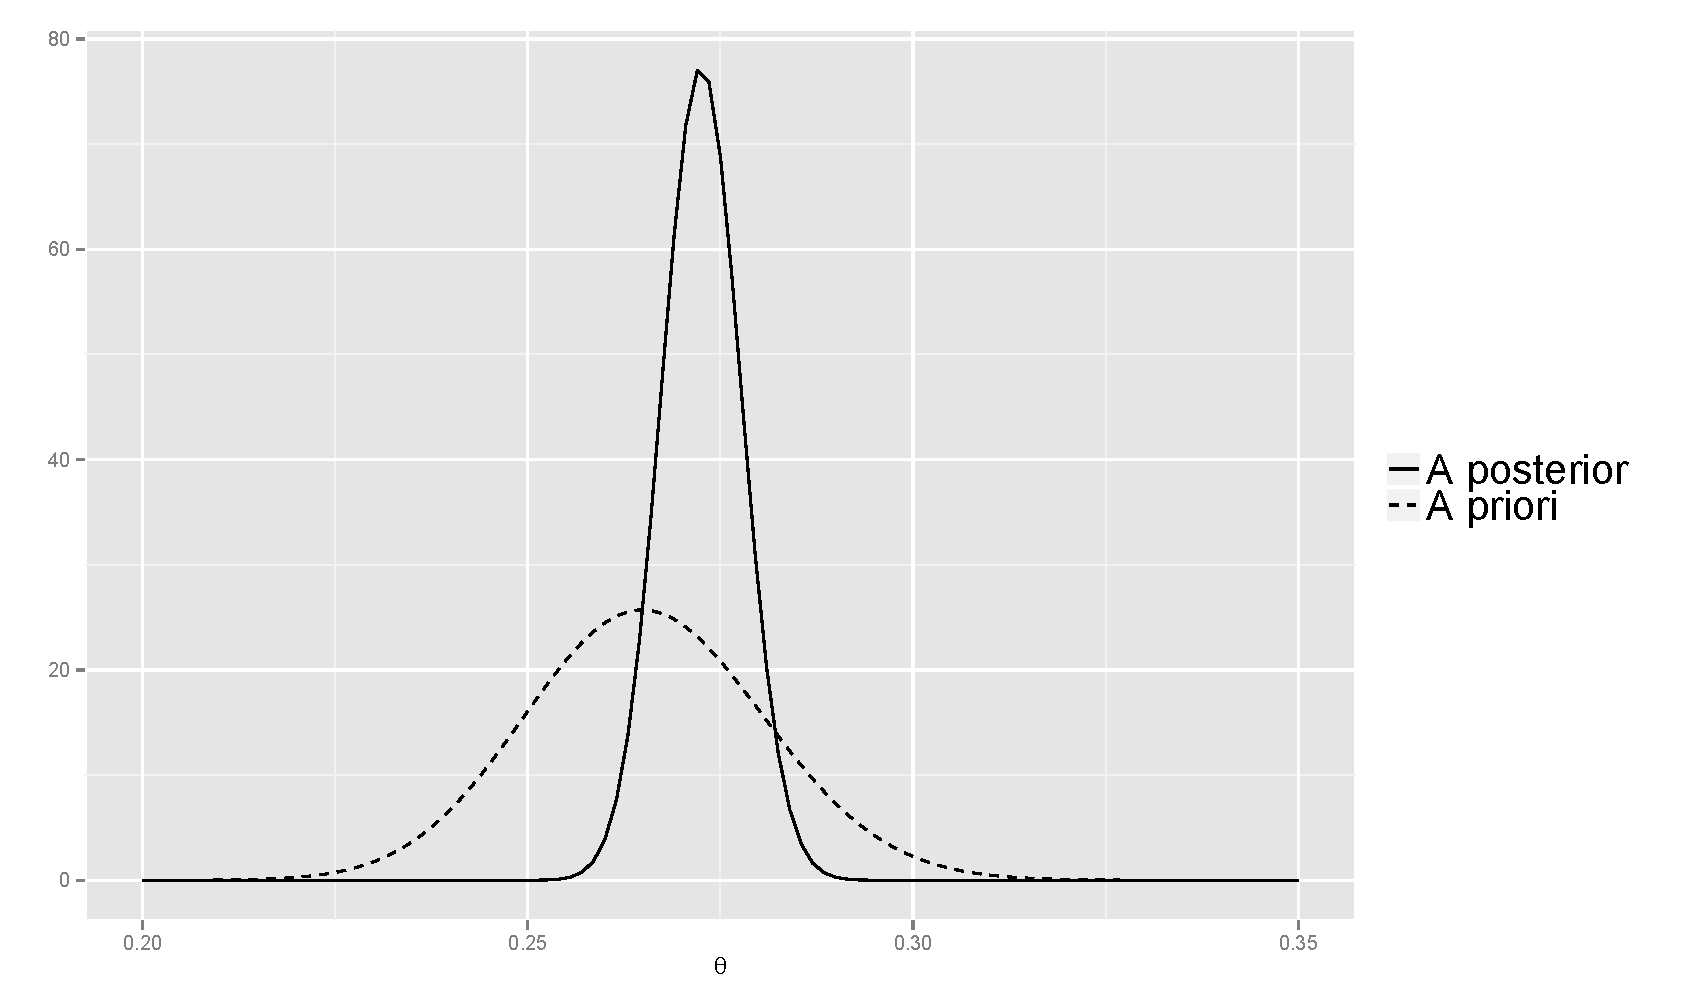
\includegraphics[scale=0.35]{BinomEj1.pdf}
    \caption{\emph{Funci\'on de densidad previa y funci\'on de densidad posterior para el ejemplo de bateo.}}
    \label{BinomEj1}
    \end{figure}
    
    Es posible analizar este conjunto de datos desde otra perspectiva al suponer que los jugadores no constituyen una muestra aleatoria y cada uno de ellos tiene un promedio de bateo diferente. Sin embargo, este an\'alisis se deja como ejercicio en un cap\'itulo posterior.
    \end{Eje}
    
    \begin{Eje}
    Continuando con el conjunto de datos de Efron y Morris, suponga que el entrenador de un equipo de las ligas inferiores est\'a interesado en adquirir los servicios de Max Alvis. Este jugador no tuvo un buen promedio de bateo en la temporada y no tuvo muchos turnos al bate. El entrenador quiere conocer cu\'al ser\'a el n\'umero m\'as probable de hits que anotar\'a en la siguiente temporada. Teniendo en cuenta que es un jugador que viene de la liga profesional, lo m\'as conveniente es que tenga muchos turnos al bate, digamos 400.
    
    Para resolver este cuestionamiento, es conveniente recurrir a la funci\'on predictiva posterior, dada en el resultado \ref{ResPredBinom} de la p\'agina \pageref{ResPredBinom}. Para este an\'alisis, se define la caracterizaci\'on estructural de la distribuci\'on previa del jugador que est\'a dada por una $Beta(\alpha=7, \beta=38)$. La siguiente funci\'on en \texttt{R} permite obtener la distribuci\'on predictiva para este jugador, que se muestra en la figura \ref{PredBinom}.
    
    \colorbox{black}{\textcolor{white}{\textbf{C\'odigo R}}}
\begin{knitrout}
\definecolor{shadecolor}{rgb}{0.933, 0.933, 0.933}\color{fgcolor}\begin{kframe}
\begin{alltt}
\hlstd{n} \hlkwb{<-} \hlnum{70}
\hlstd{s}\hlkwb{<-} \hlnum{14}
\hlstd{alp} \hlkwb{<-}\hlnum{7}
\hlstd{bet} \hlkwb{<-} \hlnum{38}
\hlstd{n.ast} \hlkwb{<-} \hlnum{400}

\hlstd{predictiva} \hlkwb{<-} \hlkwd{rep}\hlstd{(}\hlnum{NA}\hlstd{,n.ast}\hlopt{+}\hlnum{1}\hlstd{)}
\hlkwa{for}\hlstd{(k} \hlkwa{in} \hlnum{0}\hlopt{:}\hlstd{n.ast)}
\hlstd{\{}
\hlstd{predictiva[(k}\hlopt{+}\hlnum{1}\hlstd{)]} \hlkwb{<-}
\hlkwd{choose}\hlstd{(n.ast,k)}\hlopt{*}\hlkwd{beta}\hlstd{(k}\hlopt{+}\hlstd{s}\hlopt{+}\hlstd{alp,bet}\hlopt{-}\hlstd{k}\hlopt{-}\hlstd{s}\hlopt{+}\hlstd{n.ast}\hlopt{+}\hlstd{n)}\hlopt{/}\hlkwd{beta}\hlstd{(s}\hlopt{+}\hlstd{alp,bet}\hlopt{-}\hlstd{s}\hlopt{+}\hlstd{n)}
\hlstd{\}}

\hlkwd{sum}\hlstd{(predictiva)}
\end{alltt}
\begin{verbatim}
## [1] 1
\end{verbatim}
\begin{alltt}
\hlkwd{which}\hlstd{(predictiva}\hlopt{==}\hlkwd{max}\hlstd{(predictiva))}
\end{alltt}
\begin{verbatim}
## [1] 71
\end{verbatim}
\end{kframe}
\end{knitrout}
    
    \begin{figure}[!h]
    \centering
    \caption{\emph{Funci\'on de densidad predictiva posterior para el jugador Max Alvis.}}
    \label{PredBinom}
    \end{figure}
    
    
    La \'ultima l\'inea del c\'odigo computacional permite concluir que lo m\'as probable es que el jugador realice 71 hits en 400 turnos al bate, cifra que no convence al entrenador para adquirir los servicios del jugador.
    \end{Eje}
    
    \section{Modelo Binomial negativa}
    
    La distribuci\'on binomial negativa describe el n\'umero de ensayos necesarios para alcanzar un n\'umero determinado y fijo de \'exitos $k$ en una secuencia independiente de experimentos tipo Bernoulli. \'esta distribuci\'on es particularmente \'util cuando el porcentaje $\theta$ que se quiere estimar es muy peque\~no, como la proporci\'on de una poblaci\'on que padece de alguna enfermedad. La raz\'on por la que no se utiliza la distribuci\'on binomial es que al fijar el n\'umero de ensayos $n$, como el porcentaje $\theta$ es muy peque\~no, es muy probable que en en la muestra de tama\~no $n$ no se encuetre ning\'un paciente con la enfermedad; mientras que al utilizar la distribuci\'on binomial negativa, de antemano se garantiza que se obtendr\'a $k$ pacientes con la enfermedad en la muestra.
    
    Suponga que $Y$ es una variable aleatoria cuya distribuci\'on es Binomial negativa que representa el n\'umero de ensayos necesarios $y$ para alcanzar un n\'umero determinado y fijo de \'exitos $k$ en un experimento. La forma funcional de esta distribuci\'on es la siguiente
    \begin{equation}
    p(Y \mid \theta)=\binom{y-1}{k-1}\theta^k(1-\theta)^{y-k}I_{\{k,k+1,\ldots,\}}(y),
    \end{equation}
    
    As\'i como en la distribuci\'on Bernoulli y Binomial, el par\'ametro $\theta$ est\'a restringido al espacio $\Theta=[0,1]$. Luego, es admisible proponer que $\theta$ siga una distribuci\'on Beta. Por tanto, la distribuci\'on previa del par\'ametro $\theta$ est\'a dada por la expresi\'on (\ref{beta_distribution}). Bajo este marco de referencia se tienen los siguientes resultados
    
    \begin{Res}
    La distribuci\'on posterior del par\'ametro $\theta$ sigue una distribuci\'on
    \begin{equation*}
    \theta \mid Y \sim Beta(\alpha+k,\beta+y-k)
    \end{equation*}
    \end{Res}
    
    \begin{proof}
    \begin{align*}
    p(\theta \mid Y)&\propto p(Y \mid \theta)p(\theta \mid \alpha,\beta)\\
    &\propto \theta^{\alpha+k-1} (1-\theta)^{y+\beta-k-1}I_{[0,1]}(\theta)
    \end{align*}
    Por lo tanto, factorizando convenientemente, se llega a una expresi\'on id\'entica a la funci\'on de distribuci\'on de una variable aleatoria con distribuci\'on $Beta(\alpha+k,\beta+y-k)$.
    \end{proof}
    
    En algunas situaciones se puede encontrar una muestra de variables con distribuci\'on binomial negativa, por ejemplo, la entrevista de pacientes para encontrar cierta enfermedad puede llevarse a cabo en diferentes puntos de atenci\'on m\'edica o en diferentes ciudades del pa\'is. As\'i en cada punto de atenci\'on, se tendr\'a el dato correspondiente a una variable con distribuci\'on binomial negativa. El procedimiento inferencial bayesiano para estas situaciones se describe a continuaci\'on:
    
    \begin{Res}
    Cuando se tiene una sucesi\'on de variables aleatorias $Y_1,\ldots, Y_n$ independientes y con distribuci\'on $BinomialNegativa(k_i,\theta)$ $(i=1,\ldots,n)$, entonces la distribuci\'on posterior del par\'ametro de inter\'es es
    \begin{equation}
    \theta \mid Y_1,\ldots, Y_n \sim Beta(\alpha+\sum_{i=1}^n k_i,\beta+\sum_{i=1}^n y_i-\sum_{i=1}^n k_i)
    \end{equation}
    \end{Res}
    
    \begin{proof}
    Se deja como ejercicio para el lector.
    \end{proof}
    
    \begin{Eje}
    Una franquicia de investigaci\'on farmac\'eutica ha desarrollado un nuevo tratamiento farmacol\'ogico sobre pacientes diab\'eticos que padezcan, a su vez, de enfermedades card\'iacas, mejor conocidas como cardiopat\'ias, entre las que se pueden encontrar la angina de pecho, infarto de miocardio,  insuficiencia mitral, estenosis mitral, entre otras. Para evaluar el nuevo tratamiento, es necesario seleccionar una muestra, mediante el dise\~no de un experimento cl\'inico, de pacientes que tienen estas caracter\'isticas.
    
    Por otro lado, se sabe que la proporci\'on de personas que padecen de diabetes y que adem\'as tienen alg\'un tipo de condici\'on cardiaca es muy baja y es necesario obtener una estimaci\'on precisa de la proporci\'on de personas con estas condiciones. Con base en lo anteriormente expuesto, se puede pensar en seleccionar una grande de personas y utilizar un acercamiento binomial para estimar esta proporci\'on. Sin embargo, dado que la prevalencia de esta condici\'on es bastante baja, es posible que el n\'umero de personas en la muestra que presenten estas enfermedades sea nulo; por consiguiente, la estimaci\'on binomial no ser\'a, de ninguna forma, precisa.
    
    Por lo tanto, el dise\~no cl\'inico est\'a supeditado al uso de la distribuci\'on Binomial Negativa, en donde se entrevistar\'an pacientes, de una base de datos de un hospital de la ciudad asociado con la franquicia, hasta conseguir una muestra de cinco pacientes que padezcan de estas condiciones. Despu\'es de varios meses de entrevistas, se encontr\'o el quinto paciente en la entrevista n\'umero 1106.
    
    Mediante el an\'alisis bayesiano, suponiendo una distribuci\'on previa $Beta(0.5, 0.5)$, se llega a que la distribuci\'on posterior del par\'ametrtos $\theta$ es $Beta(0.5+5, 0.5+1106-5)=Beta(5.5, 1101.5)$. Por lo tanto, la estimaci\'on puntual del par\'ametro de inter\'es, que corresponde a la media de la distribuci\'on posterior, es 0.0049, que equivale una proporci\'on de 0.49\% de personas con estas enfermedades. El siguiente c\'odigo computacional muestra c\'omo se puede llegar a las mismas conclusiones con JAGS
    
    \colorbox{black}{\textcolor{white}{\textbf{C\'odigo JAGS}}}
\begin{knitrout}
\definecolor{shadecolor}{rgb}{0.933, 0.933, 0.933}\color{fgcolor}\begin{kframe}
\begin{alltt}
\hlstd{BinNeg.model} \hlkwb{<-} \hlkwa{function}\hlstd{()\{}
\hlstd{y} \hlopt{~} \hlkwd{dnegbin}\hlstd{(theta,}\hlnum{5}\hlstd{)}
\hlstd{theta}\hlopt{~}\hlkwd{dbeta}\hlstd{(}\hlnum{0.5}\hlstd{,} \hlnum{0.5}\hlstd{)}
\hlstd{\}}

\hlcom{#BinNeg.data <- }
\hlcom{#list(y =1106)}
\hlstd{BinNeg.param} \hlkwb{<-} \hlkwd{c}\hlstd{(}\hlstr{"theta"}\hlstd{)}
\hlstd{BinNeg.inits} \hlkwb{<-} \hlkwa{function}\hlstd{()\{}
\hlkwd{list}\hlstd{(}\hlstr{"theta"}\hlstd{=}\hlnum{0.5}\hlstd{)}
\hlstd{\}}

\hlstd{BinNeg.fit} \hlkwb{<-} \hlkwd{jags}\hlstd{(}\hlkwc{data}\hlstd{=}\hlkwd{list}\hlstd{(}\hlkwc{y}\hlstd{=}\hlnum{1106}\hlstd{),}\hlkwc{inits}\hlstd{=BinNeg.inits,BinNeg.param,}\hlkwc{n.iter}\hlstd{=}\hlnum{10000}\hlstd{,}\hlkwc{n.burn}\hlstd{=}\hlnum{1000}\hlstd{,}\hlkwc{model.file}\hlstd{=BinNeg.model)}
\end{alltt}
\begin{verbatim}
## Compiling model graph
##    Resolving undeclared variables
##    Allocating nodes
## Graph information:
##    Observed stochastic nodes: 1
##    Unobserved stochastic nodes: 1
##    Total graph size: 5
## 
## Initializing model
\end{verbatim}
\begin{alltt}
\hlkwd{print}\hlstd{(BinNeg.fit)}
\end{alltt}
\begin{verbatim}
## Inference for Bugs model at "/var/folders/n7/01szs8_x7pq1bvpwwnvq7w_w0000gn/T//RtmpMtD1jH/model11b725be15f2.txt", fit using jags,
##  3 chains, each with 10000 iterations (first 1000 discarded), n.thin = 9
##  n.sims = 3000 iterations saved
##          mu.vect sd.vect   2.5%    25%    50%    75% 97.5%  Rhat n.eff
## theta      0.005   0.002  0.002  0.003  0.005  0.006  0.01 1.001  2300
## deviance  15.256   1.314 14.284 14.383 14.715 15.616 18.96 1.001  3000
## 
## For each parameter, n.eff is a crude measure of effective sample size,
## and Rhat is the potential scale reduction factor (at convergence, Rhat=1).
## 
## DIC info (using the rule, pD = var(deviance)/2)
## pD = 0.9 and DIC = 16.1
## DIC is an estimate of expected predictive error (lower deviance is better).
\end{verbatim}
\end{kframe}
\end{knitrout}
    
    Despu\'es de cinco mil iteraciones, la salida del anterior c\'odigo muestra la estimaci\'on puntual dada por 0.004956 y un intervalo de credibilidad al 95\%, dado por $(0.001766, 0.009931)$.
    \end{Eje}
    
    \begin{Eje}
    Continuando con la tem\'atica del ejemplo anterior, suponga que la franquicia llev\'o a cabo la misma investigaci\'on en las 31 ciudades con mayor densidad poblacional de pa\'is. Como en la mayor\'ia de los casos, debido al condicionamiento presupuestal, el experimento difiri\'o en el n\'umero de \'exitos en cada caso. En total, se tuvieron 29620 entrevistas para un total de \'exitos de 152, tal como se muestra a continuaci\'on.
    
    \begin{center}
    \begin{verbatim}
    Ciudad                 y          k
    
    BOGOTA               1001         4
    MEDELLIN             978          6
    CALI                 999          5
    BARRANQUILLA         860          4
    CARTAGENA            1155         4
    CUCUTA               585          6
    BUCARAMANGA          1030         3
    IBAGUE               960          5
    SOLEDAD              1002         6
    SANTA MARTA          763          7
    SOACHA               1036         5
    PASTO                779          5
    MONTERIA             1158         4
    VILLAVICENCIO        1017         5
    BELLO                888          6
    MANIZALES            977          4
    VALLEDUPAR           1256         6
    BUENAVENTURA         1349         6
    NEIVA                1047         5
    PALMIRA              1088         5
    ARMENIA              649          3
    POPAYAN              765          4
    FLORIDABLANCA        699          5
    SINCELEJO            1042         4
    ITAGUI               1212         5
    BARRANCABERMEJA      660          5
    TULUA                671          5
    ENVIGADO             835          6
    DOSQUEBRADAS         997          5
    RIOHACHA             1146         4
    SINCELEJO            1016         5 
    \end{verbatim}
    \end{center}
    
    Mediante el an\'alisis bayesiano, suponiendo una distribuci\'on previa\footnote{N\'otese que es posible tambi\'en asignar una previa informativa $Beta(5.5, 1101.5)$, que da cuenta de la informaci\'on del estudio del ejemplo anterior.} no informativa $Beta(0.5, 0.5)$, se llega a que la distribuci\'on posterior del par\'ametrtos $\theta$ es $Beta(0.5+152, 0.5+29620-152)=Beta(152.5, 29468.5)$. Por lo tanto, la estimaci\'on puntual del par\'ametro de inter\'es, que corresponde a la media de la distribuci\'on posterior, es 0.0051, que equivale una proporci\'on de 0.51\% de personas con estas enfermedades. El siguiente c\'odigo computacional muestra c\'omo se puede llegar a las mismas conclusiones con JAGS
    
    \colorbox{black}{\textcolor{white}{\textbf{C\'odigo JAGS}}}
\begin{knitrout}
\definecolor{shadecolor}{rgb}{0.933, 0.933, 0.933}\color{fgcolor}\begin{kframe}
\begin{alltt}
\hlstd{BinNeg2.model} \hlkwb{<-} \hlkwa{function}\hlstd{()\{}
\hlkwa{for}\hlstd{(i} \hlkwa{in} \hlnum{1}\hlopt{:}\hlnum{31}\hlstd{)\{}
\hlstd{y[i]}\hlopt{~}\hlkwd{dnegbin}\hlstd{(theta,k[i])}
\hlstd{\}}
\hlstd{theta} \hlopt{~} \hlkwd{dbeta}\hlstd{(}\hlnum{0.5}\hlstd{,} \hlnum{0.5}\hlstd{)}
\hlstd{\}}

\hlstd{y} \hlkwb{<-} \hlkwd{c}\hlstd{(}\hlnum{1001}\hlstd{,} \hlnum{978}\hlstd{,} \hlnum{999}\hlstd{,} \hlnum{860}\hlstd{,} \hlnum{1155}\hlstd{,} \hlnum{585}\hlstd{,} \hlnum{1030}\hlstd{,} \hlnum{960}\hlstd{,} \hlnum{1002}\hlstd{,} \hlnum{763}\hlstd{,} \hlnum{1036}\hlstd{,} \hlnum{779}\hlstd{,} \hlnum{1158}\hlstd{,} \hlnum{1017}\hlstd{,} \hlnum{888}\hlstd{,} \hlnum{977}\hlstd{,} \hlnum{1256}\hlstd{,} \hlnum{1349}\hlstd{,} \hlnum{1047}\hlstd{,} \hlnum{1088}\hlstd{,} \hlnum{649}\hlstd{,} \hlnum{765}\hlstd{,} \hlnum{699}\hlstd{,} \hlnum{1042}\hlstd{,} \hlnum{1212}\hlstd{,} \hlnum{660}\hlstd{,} \hlnum{671}\hlstd{,} \hlnum{835}\hlstd{,} \hlnum{997}\hlstd{,} \hlnum{1146}\hlstd{,} \hlnum{1016}\hlstd{)}
\hlstd{k} \hlkwb{<-} \hlkwd{c}\hlstd{(}\hlnum{4}\hlstd{,} \hlnum{6}\hlstd{,} \hlnum{5}\hlstd{,} \hlnum{4}\hlstd{,} \hlnum{4}\hlstd{,} \hlnum{6}\hlstd{,} \hlnum{3}\hlstd{,} \hlnum{5}\hlstd{,} \hlnum{6}\hlstd{,} \hlnum{7}\hlstd{,} \hlnum{5}\hlstd{,} \hlnum{5}\hlstd{,} \hlnum{4}\hlstd{,} \hlnum{5}\hlstd{,} \hlnum{6}\hlstd{,} \hlnum{4}\hlstd{,} \hlnum{6}\hlstd{,} \hlnum{6}\hlstd{,} \hlnum{5}\hlstd{,} \hlnum{5}\hlstd{,} \hlnum{3}\hlstd{,} \hlnum{4}\hlstd{,} \hlnum{5}\hlstd{,} \hlnum{4}\hlstd{,} \hlnum{5}\hlstd{,} \hlnum{5}\hlstd{,} \hlnum{5}\hlstd{,} \hlnum{6}\hlstd{,} \hlnum{5}\hlstd{,} \hlnum{4}\hlstd{,} \hlnum{5}\hlstd{)}

\hlstd{BinNeg2.data} \hlkwb{<-} \hlkwd{list}\hlstd{(}\hlstr{"y"}\hlstd{,} \hlstr{"k"}\hlstd{)}
\hlstd{BinNeg2.param} \hlkwb{<-} \hlkwd{c}\hlstd{(}\hlstr{"theta"}\hlstd{)}
\hlstd{BinNeg2.inits} \hlkwb{<-} \hlkwa{function}\hlstd{()\{}
\hlkwd{list}\hlstd{(}\hlstr{"theta"}\hlstd{=}\hlnum{0.5}\hlstd{)}
\hlstd{\}}
\hlstd{BinNeg2.fit} \hlkwb{<-} \hlkwd{jags}\hlstd{(}\hlkwc{data}\hlstd{=BinNeg2.data,} \hlkwc{inits}\hlstd{=BinNeg2.inits, BinNeg2.param,} \hlkwc{n.iter}\hlstd{=}\hlnum{10000}\hlstd{,} \hlkwc{n.burnin}\hlstd{=}\hlnum{1000}\hlstd{,} \hlkwc{model.file}\hlstd{=BinNeg2.model)}
\end{alltt}
\begin{verbatim}
## Compiling model graph
##    Resolving undeclared variables
##    Allocating nodes
## Graph information:
##    Observed stochastic nodes: 31
##    Unobserved stochastic nodes: 1
##    Total graph size: 65
## 
## Initializing model
\end{verbatim}
\begin{alltt}
\hlkwd{print}\hlstd{(BinNeg2.fit)}
\end{alltt}
\begin{verbatim}
## Inference for Bugs model at "/var/folders/n7/01szs8_x7pq1bvpwwnvq7w_w0000gn/T//RtmpMtD1jH/model11b7162e6abe.txt", fit using jags,
##  3 chains, each with 10000 iterations (first 1000 discarded), n.thin = 9
##  n.sims = 3000 iterations saved
##          mu.vect sd.vect    2.5%     25%     50%     75%   97.5%  Rhat
## theta      0.005   0.000   0.004   0.005   0.005   0.005   0.006 1.001
## deviance 447.039   1.434 446.050 446.149 446.496 447.333 451.152 1.001
##          n.eff
## theta     2800
## deviance  3000
## 
## For each parameter, n.eff is a crude measure of effective sample size,
## and Rhat is the potential scale reduction factor (at convergence, Rhat=1).
## 
## DIC info (using the rule, pD = var(deviance)/2)
## pD = 1.0 and DIC = 448.1
## DIC is an estimate of expected predictive error (lower deviance is better).
\end{verbatim}
\end{kframe}
\end{knitrout}
    
    Despu\'es de cinco mil iteraciones, la salida del anterior c\'odigo muestra la estimaci\'on puntual dada por 0.005121 y un intervalo de credibilidad al 95\%, dado por $(0.004335, 0.005956)$, mucho m\'as estrecho que el intervalo de credibilidad del anterior ejercicio.
    \end{Eje}
    
    Una vez observados los datos actuales y encontrada la distribuci\'on posterior, se puede encontrar la distribuci\'on predictiva posterior de una nueva variable con distribuci\'on binomial negativa. Es decir, se puede definir el mecanismo probabil\'istico para el n\'umero de ensayos necesarios para encontrar $\tilde{k}$ \'exitos.
    \begin{Res}
    Despu\'es de la recolecci\'on de datos, la distribuci\'on predictiva posterior para una nueva variable $\tilde{Y}$ est\'a dada por
    \begin{equation*}
    p(\tilde{Y}|Y_1,\cdots,Y_n)=\binom{\tilde{y}-1}{\tilde{k}-1}\frac{Beta(\alpha+\tilde{k}+\sum k_i,\beta+\tilde{y}-\tilde{k}+\sum y_i-\sum k_i)}{Beta(\alpha+\sum k_i,\beta+\sum y_i-\sum k_i)}I_{\{\tilde{k},\tilde{k}+1,\cdots\}}(\tilde{y})
    \end{equation*}
    \end{Res}
    
    \begin{proof}
    \begin{align*}
    &\ \ \ p(\tilde{Y}|Y_1,\cdots,Y_n)\\
    &=\int p(\tilde{Y}|\theta)p(\theta|Y_1,\cdots,Y_n)d\theta\\
    &=\int_{0}^1\binom{\tilde{y}-1}{\tilde{k}-1}\theta^{\alpha+\tilde{k}}(1-\theta)^{\beta+\tilde{y}-\tilde{k}}I_{\{\tilde{k},\tilde{k}+1,\cdots\}}(\tilde{y})\frac{\theta^{\sum k_i-1}(1-\theta)^{\sum y_i-\sum k_i-1}}{Beta(\alpha+\sum k_i,\beta+\sum y_i-\sum k_i)}d\theta\\
    &=\binom{\tilde{y}-1}{\tilde{k}-1}\frac{I_{\{\tilde{k},\tilde{k}+1,\cdots\}}(\tilde{y})}{Beta(\alpha+\sum k_i,\beta+\sum y_i-\sum k_i)}\int_{0}^1\theta^{\alpha+\tilde{k}+\sum k_i-1}(1-\theta)^{\beta+\tilde{y}-\tilde{k}+\sum y_i-\sum k_i-1}d\theta\\
    &=\binom{\tilde{y}-1}{\tilde{k}-1}\frac{Beta(\alpha+\tilde{k}+\sum k_i,\beta+\tilde{y}-\tilde{k}+\sum y_i-\sum k_i)}{Beta(\alpha+\sum k_i,\beta+\sum y_i-\sum k_i)}I_{\{\tilde{k},\tilde{k}+1,\cdots\}}(\tilde{y})
    \end{align*}
    \end{proof}
    
    \begin{Eje}
    Siguiendo con los datos del Ejemplo 2.3.2, suponga que se quiere recolectar informaci\'on de 3 pacientes con cardiopat\'ia en cierta ciudad, y se quiere conocer acerca del n\'umero de entrevistas necesarias. Utilizando la distribuci\'on previa $Beta(0.5,0.5)$ y los datos de las 31 ciudades del ejemplo, se tiene que la distribuci\'on predictiva para el n\'umero de entrevistas necesarias para encontrar 3 pacientes est\'a dada por
    \begin{align*}
    &\ \ \ \ p(\tilde{Y}|Y_1,\cdots,Y_n)\\
    &=\binom{\tilde{y}-1}{4}\frac{Beta(0.5+5+152,0.5+\tilde{y}-5+29620-152)}{Beta(0.5+152,0.5+29620-152)}I_{\{5,6,\cdots\}}(\tilde{y})\\
    &=\binom{\tilde{y}-1}{4}\frac{Beta(157.5,\tilde{y}+29463.5)}{Beta(152.5,29468.5)}I_{\{5,6,\cdots\}}(\tilde{y})
    \end{align*}
    
    Con los siguientes c\'odigos se puede calcular la anterior funci\'on predictiva.
    
    \colorbox{black}{\textcolor{white}{\textbf{C\'odigo R}}}
\begin{knitrout}
\definecolor{shadecolor}{rgb}{0.933, 0.933, 0.933}\color{fgcolor}\begin{kframe}
\begin{alltt}
\hlstd{predict}\hlkwb{<-}\hlkwa{function}\hlstd{(}\hlkwc{y}\hlstd{,}\hlkwc{alfa}\hlstd{,}\hlkwc{beta}\hlstd{,}\hlkwc{s}\hlstd{,}\hlkwc{n}\hlstd{,}\hlkwc{k}\hlstd{)\{}
\hlkwd{choose}\hlstd{(y}\hlopt{-}\hlnum{1}\hlstd{,k}\hlopt{-}\hlnum{1}\hlstd{)}\hlopt{*}\hlkwd{exp}\hlstd{(}\hlkwd{lbeta}\hlstd{(alfa}\hlopt{+}\hlstd{k}\hlopt{+}\hlstd{s,beta}\hlopt{+}\hlstd{y}\hlopt{-}\hlstd{k}\hlopt{+}\hlstd{n}\hlopt{-}\hlstd{s)}\hlopt{-}\hlkwd{lbeta}\hlstd{(alfa}\hlopt{+}\hlstd{s,beta}\hlopt{+}\hlstd{n}\hlopt{-}\hlstd{s))}
\hlstd{\}}

\hlstd{alfa} \hlkwb{<-} \hlstd{beta} \hlkwb{<-} \hlnum{0.5}
\hlstd{s} \hlkwb{<-} \hlnum{152}\hlstd{;n} \hlkwb{<-} \hlnum{29620}\hlstd{;k} \hlkwb{<-} \hlnum{5}
\hlstd{fun} \hlkwb{<-} \hlkwd{rep}\hlstd{(}\hlnum{NA}\hlstd{)}
\hlkwa{for}\hlstd{(y} \hlkwa{in} \hlnum{5}\hlopt{:}\hlnum{5000}\hlstd{)\{}
\hlstd{fun[y}\hlopt{-}\hlnum{4}\hlstd{]} \hlkwb{<-} \hlkwd{predict}\hlstd{(y,alfa,beta,s,n,k)}
\hlstd{\}}
\hlkwd{sum}\hlstd{(fun)}
\end{alltt}
\begin{verbatim}
## [1] 1
\end{verbatim}
\end{kframe}
\end{knitrout}
    
    \begin{figure}[!htb]\label{jefber}
    \centering
    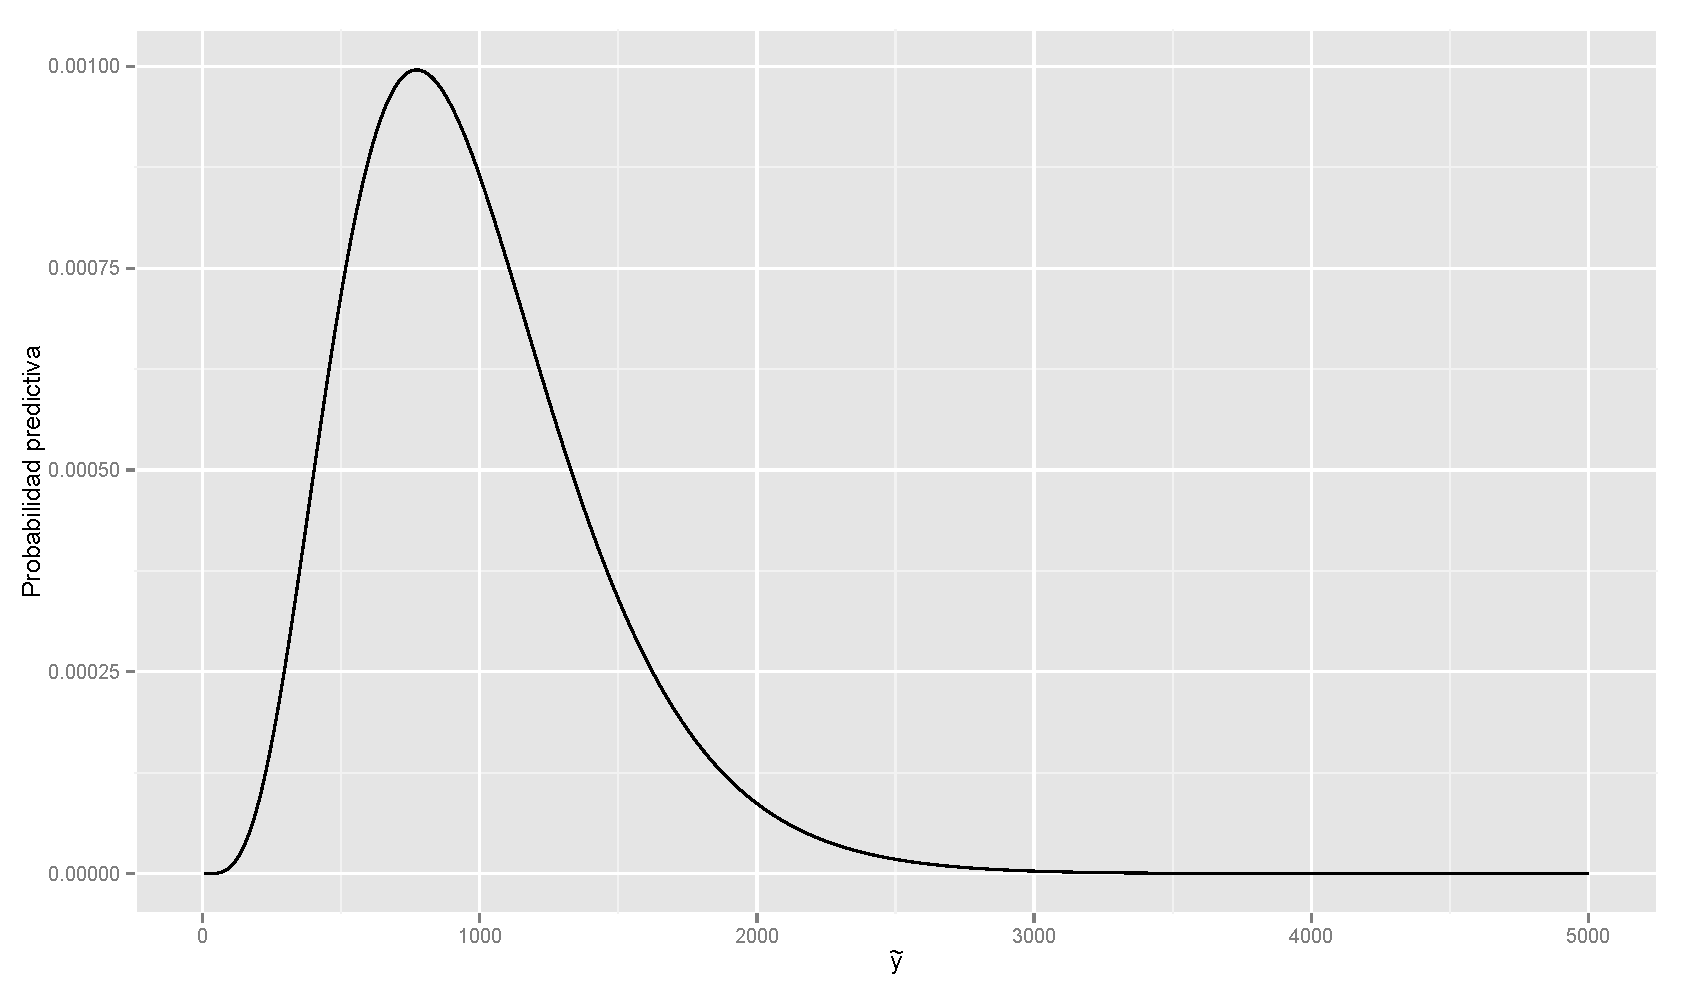
\includegraphics[scale=0.35]{pred_negabinom.pdf}
    \caption{\emph{Distribuci\'on predictiva posterior para el n\'umero de entrevistas necesarias para encontrar 5 pacientes usando los datos del ejemplo 2.3.2}}
    \end{figure}
    
    Se puede ver que el n\'umero de entrevistas que tiene mayor probabilidad asociadas es el valor 772, usando el comando
\begin{knitrout}
\definecolor{shadecolor}{rgb}{0.933, 0.933, 0.933}\color{fgcolor}\begin{kframe}
\begin{alltt}
\hlkwd{which}\hlstd{(fun}\hlopt{==}\hlkwd{max}\hlstd{(fun))}\hlopt{+}\hlnum{4}
\end{alltt}
\begin{verbatim}
## [1] 772
\end{verbatim}
\end{kframe}
\end{knitrout}
    Tambi\'en, se puede calcular la probabilidad de que en menos de 500 entrevistas se encuentren los 5 pacientes es de solo el 12\% usando el comando
\begin{knitrout}
\definecolor{shadecolor}{rgb}{0.933, 0.933, 0.933}\color{fgcolor}\begin{kframe}
\begin{alltt}
\hlkwd{sum}\hlstd{(fun[}\hlnum{1}\hlopt{:}\hlstd{(}\hlnum{500}\hlopt{-}\hlnum{4}\hlstd{)])}
\end{alltt}
\begin{verbatim}
## [1] 0.1201
\end{verbatim}
\end{kframe}
\end{knitrout}
    \end{Eje}
    
    \section{Modelo Poisson}
    
    Suponga que $\mathbf{Y}=\{Y_1,\ldots,Y_n\}$ es una muestra aleatoria de variables con distribuci\'on Poisson con par\'ametro $\theta$, la funci\'on de distribuci\'on conjunta o la funci\'on de verosimilitud est\'a dada por
    \begin{align*}
    p(\mathbf{Y} \mid \theta)&=\prod_{i=1}^n\frac{e^{-\theta}\theta^{y_i}}{y_i!}I_{\{0,1,\ldots\}}(y_i)\\
    &=\frac{e^{-n\theta}\theta^{\sum_{i=1}^ny_i}}{\prod_{i=1}^ny_i!}I_{\{0,1,\ldots\}^n}(y_1,\ldots,y_n)
    \end{align*}
    
    donde $\{0,1\ldots\}^n$ denota el producto cartesiano $n$ veces sobre el conjunto $\{0,1\ldots\}$. Por otro lado, como el par\'ametro $\theta$ est\'a restringido al espacio $\Theta=(0,\infty)$, entonces es posible formular varias opciones para la distribuci\'on previa del par\'ametro. Algunas opciones se encuentran considerando la distribuci\'on exponencial o la distribuci\'on chi-cuadrado o la distribuci\'on Gamma. N\'otese que las dos primeras distribuciones son casos particulares de la \'ultima. Por lo tanto, la distribuci\'on previa del par\'ametro $\theta$ est\'a dada por
    \begin{equation}
    p(\theta \mid \alpha,\beta)=\frac{\beta^\alpha}{\Gamma(\alpha)}\theta^{\alpha-1} e^{-\beta\theta}I_{(0,\infty)}(\theta).
    \end{equation}
    
    Bajo este marco de referencia se tienen el siguiente resultado con respecto a la distribucion posterior del par\'ametro de inter\'es $\theta$.
    \begin{Res}
    \label{ResPoissonPost}
    La distribuci\'on posterior del par\'ametro $\theta$ est\'a dada por
    \begin{equation*}
    \theta \mid \mathbf{Y} \sim Gamma\left(\sum_{i=1}^ny_i+\alpha,n+\beta\right)
    \end{equation*}
    \end{Res}
    
    \begin{proof}
    \begin{align*}
    p(\theta \mid \mathbf{Y})&\propto p(\mathbf{Y} \mid \theta)p(\theta \mid \alpha,\beta)\\
    &=\frac{I_{\{0,1,\ldots\}^n}(y_1,\ldots,y_n)}{\prod_{i=1}^ny_i!}\frac{\beta^\alpha}{\Gamma(\alpha)}
    \theta^{\alpha-1}\theta^{\sum_{i=1}^ny_i}e^{-\beta\theta}e^{-n\theta}I_{(0,\infty)}(\theta)\\
    &\propto \theta^{\sum_{i=1}^ny_i+\alpha-1}e^{-(\beta+n)\theta}I_{(0,\infty)}(\theta)
    \end{align*}
    Por lo tanto, factorizando convenientemente, se encuentra una expresi\'on id\'entica a la funci\'on de distribuci\'on de una variable aleatoria con distribuci\'on $Gamma(\sum_{i=1}^ny_i+\alpha,n+\beta)$.
    \end{proof}
    
    Utilizando el resultado anterior, se tiene que la estimaci\'on Bayesiana del par\'ametro $\theta$ est\'a dada por
    \begin{equation*}
    \hat{\theta}=\frac{\sum_{i=1}^ny_i+\alpha}{n+\beta}.
    \end{equation*}
    
    La anterior expresi\'on sugiere tomar los par\'ametros de la distribuci\'on previa $\alpha$ y $\beta$ de la siguiente manera: $\beta$ representa el n\'umero de observaciones en la informaci\'on previa, mientras que $\alpha$ representa la suma de los datos de la informaci\'on previa. De esta forma, $\alpha/\beta$ representa la estimaci\'on previa del par\'ametro $\theta$. Y la estimaci\'on Bayesiana de $\theta$ se puede escribir como
    \begin{align*}
    \hat{\theta}&=\frac{\sum_{i=1}^ny_i+\alpha}{\beta+n}\\
    &=\frac{n}{n+\beta}*\frac{\sum y_i}{n}+\frac{\beta}{n+\beta}*\frac{\alpha}{\beta}\\
    &=\frac{n}{n+\beta}*\hat{\theta_C}+\frac{\beta}{n+\beta}*\hat{\theta_P}\\
    \end{align*}
    Es decir, la estimaci\'on Bayesiana de $\theta$ es un promedio ponderado entre la estimaci\'on cl\'asica y la estimaci\'on previa del par\'ametro $\theta$, donde los pesos dependen directamente del tama\~no muestral de la informaci\'on actual y de la informaci\'on previa. 
    
    A continuaci\'on estudiamos las distribuciones predictivas previa y posterior de una nueva observaci\'on 
    \begin{Res}
    La distribuci\'on predictiva previa para una observaci\'on $\mathbf{y}=\{y_1,\ldots,y_n\}$ de la muestra aleatoria est\'a dada por
    \begin{equation}\label{Pre_prior_Poisson}
    p(\mathbf{Y})=\frac{\Gamma(\sum_{i=1}^ny_i+\alpha)}{\Gamma(\alpha)}\frac{\beta^\alpha}{(n+\beta)^{\sum_{i=1}^ny_i+\alpha}}
    \frac{I_{\{0,1,\ldots\}^n}(y_1,\ldots,y_n)}{\prod_{i=1}^ny_i!}
    \end{equation}
    y define una aut\'entica funci\'on de densidad de probabilidad continua.
    \end{Res}
    
    \begin{proof}
    De la definici\'on de funci\'on de distribuci\'on predictiva se tiene que 
    \begin{align*}
    p(\mathbf{Y})&=\int p(\mathbf{Y} \mid \theta)p(\theta \mid \alpha,\beta)\ d\theta\\
    &=\int_0^{\infty} \frac{e^{-n\theta}\theta^{\sum_{i=1}^ny_i}}{\prod_{i=1}^ny_i!}I_{\{0,1,\ldots\}^n}(y_1,\ldots,y_n)
    \frac{\beta^\alpha \theta^{\alpha-1} e^{-\beta\theta}}{\Gamma(\alpha)}\ d\theta\\
    &=\frac{\Gamma(\sum_{i=1}^ny_i+\alpha)}{\Gamma(\alpha)}\frac{\beta^\alpha}{(n+\beta)^{\sum_{i=1}^ny_i+\alpha}}
    \frac{I_{\{0,1,\ldots\}^n}(y_1,\ldots,y_n)}{\prod_{i=1}^ny_i!}\\
    &\hspace{2cm}\times
    \int_0^{\infty} \frac{(n+\beta)^{\sum_{i=1}^ny_i+\alpha}}{\Gamma(\sum_{i=1}^ny_i+\alpha)}
    \theta^{\sum_{i=1}^ny_i+\alpha-1}e^{-(\beta+n)\theta} \ d\theta\\
    &=\frac{\Gamma(\sum_{i=1}^ny_i+\alpha)}{\Gamma(\alpha)}\frac{\beta^\alpha}{(n+\beta)^{\sum_{i=1}^ny_i+\alpha}}
    \frac{I_{\{0,1,\ldots\}^n}(y_1,\ldots,y_n)}{\prod_{i=1}^ny_i!}
    \end{align*}
    \end{proof}
    
    En el caso en que la muestra aleatoria estuviera constituida por una sola variable aleatoria, entonces $n=1$ y si, en particular, los hiper-par\'ametros de la distribuci\'on previa fuesen $\alpha=\beta=1$, entonces no es dif\'icil ver, utilizando la definici\'on de la funci\'on matem\'atica Gamma, que la funci\'on de distribuci\'on predictiva (\ref{Pre_prior_Poisson}) estar\'ia dada por
    \begin{align}\label{Pre_prior_poisson1}
    p(Y)&=\frac{\Gamma(y+1)}{\Gamma(1)}\frac{1}{2^{y+1}}\frac{I_{\{0,1,\ldots\}}(y)}{y!} \notag\\
    &=\frac{1}{2^{y+1}}I_{\{0,1,\ldots\}}(y)
    \end{align}
    
    Para chequear la convergencia de la anterior distribuci\'on es necesario recurrir a los resultados del an\'alisis matem\'atico \cite[p. 361]{Apostol}. Dado que el espacio de muestreo de la variable aleatoria $Y$ es $\{0,1,\ldots\}$, entonces la suma infinita converge a uno lo que conlleva a que, en este caso particular, $P(Y)$ sea una aut\'entica funci\'on de densidad de probabilidad.
    \begin{align*}
    \sum_{y=0}^{\infty}p(Y=y)=\sum_{y=0}^{\infty}\left(\frac{1}{2}\right)^{y+1}=\frac{1}{2}\sum_{y=0}^{\infty}\left(\frac{1}{2}\right)^{y}
    =\frac{1}{2}\frac{1}{1-1/2}=1
    \end{align*}
    
    y podemos afirmar que la expresion (\ref{Pre_prior_poisson1}) s\'i representa una funci\'on de densidad de una variable discreta. Ahora, consideramos la distribuci\'on predictiva poseterior de una muestra aleatoria, esta distribuci\'on se presenta en el siguiente resultado.
    
    \begin{Res}
    \label{ResPoissonPred}
    Despu\'es de la recolecci\'on de los datos, la distribuci\'on predictiva posterior para una nueva posible observaci\'on $\tilde{\mathbf{y}}=\{\tilde{y}_1,\ldots,\tilde{y}_{n^*}\}$, de tama\~no $n^*$, est\'a dada por
    
    \begin{align}
    p(\tilde{\mathbf{y}} \mid \mathbf{Y})&=\frac{\Gamma(\sum_{i=1}^{n^*}\tilde{y}_i+\sum_{i=1}^ny_i+\alpha)}{\Gamma(\sum_{i=1}^ny_i+\alpha)}
    \frac{(\beta+n)^{\sum_{i=1}^ny_i+\alpha}}{({n^*}+\beta+n)^{\sum_{i=1}^{n^*}\tilde{y}_i+\sum_{i=1}^ny_i+\alpha}}\notag\\
    &\hspace{5cm}\times
    \frac{I_{\{0,1,\ldots\}^{n^*}}(\tilde{y}_1,\ldots,\tilde{y}_{n^*})}{\prod_{i=1}^{n^*}\tilde{y}_i!}
    \end{align}
    \end{Res}
    
    \begin{proof}
    De la definici\'on de funci\'on de distribuci\'on predictiva, y haciendo uso del mismo razonamiento en la demostraci\'on del Resultado 2.1.8, se tiene la prueba inmediata.
    \end{proof}
    
    La anterior distribuci\'on corresponde a una distribucion multivariada que nos permite calcular probabilidades predictivas para cualesquieras valores de $\tilde{y}_1$, $\cdots$, $\tilde{y}_{n^*}$; sin embargo, en algunas situaciones, como por ejemplo, cuando $\theta$ representa el n\'umero promedio de alg\'un suceso en una regi\'on geogr\'afica, entonces al momento de la predicci\'on, podemos estar interesados en predecir el n\'umero total o el n\'umero promedio de sucesos en la nueva muestra aleatoria de regiones geogr\'aficos. Es decir, podemos estar m\'as interesados en la distribuci\'on de $\sum_{y=1}^{n^*} \tilde{y}_i$ o de $\sum_{y=1}^{n^*} \tilde{y}_i/n^*$ en vez de la distribuci\'on conjunta de $\tilde{y}_1$, $\cdots$, $\tilde{y}_{n^*}$. La distribuci\'on predictiva de $\sum_{y=1}^{n^*} \tilde{y}_i$ se presenta en el siguiente resultado, y con esta distribuci\'on se puede obtener f\'acilmente probabilidades predictivas para $\sum_{y=1}^{n^*} \tilde{y}_i/n^*$.
    
    \begin{Res}
    Despu\'es de la recolecci\'on de los datos, la distribuci\'on predictiva posterior para la suma de un vector de observaciones nuevas $\left(\tilde{y}_1,\ldots,\tilde{y}_{n^*}\right)$, $\tilde{s} = \sum_{y=1}^{n^*} \tilde{y}_i$, est\'a dada por:
    
    \begin{align}\label{pre_pos_poisson_sum}
    p(\tilde{\mathbf{s}} \mid \mathbf{Y})&=\frac{\Gamma(\tilde{s}+\sum_{i=1}^ny_i+\alpha)}{\Gamma(\sum_{i=1}^ny_i+\alpha)}
    \frac{(n+\beta)^{\sum_{i=1}^ny_i+\alpha}}{({n^*}+n+\beta)^{\tilde{s}+\sum_{i=1}^ny_i+\alpha}}\frac{(n^*)^{\tilde{s}}I_{\{0,1,\ldots\}}(\tilde{s})}{\tilde{s}!}
    \end{align}
    \end{Res}
    
    \begin{proof}
    Usando el hecho de que $\theta|\mathbf{Y}\sim Gamma(\sum_{i=1}^{n}y_i+\alpha,n+\beta)$ y $\tilde{s}|\theta\sim Poisson(n^*\theta)$ se procede a calcular $\tilde{s}/p(\mathbf{y})$,
    as\'i:
    \begin{align*}
    &\ \ \ \ p(\tilde{s}|\mathbf{y}) \\
    &= \int_{\Omega} p(\tilde{s}|\theta)p(\theta|\mathbf{y})d\theta\\
    & = \int_{\Omega} \frac{(n^{*}\theta)^{\tilde{s}}e^{-n^*\theta}}{\tilde{s}!} I_{\{0,1,\ldots\}}(\tilde{s}) (\beta+n)^{\sum_{i=1}^{n}y_i+\alpha}\frac{\theta^{\tilde{s}+\sum_{i=1}^{n}y_i+\alpha-1}}{\Gamma(\sum_{i=1}^{n}y_i+\alpha)}e^{-(\beta+n)\theta}I_{(0,\infty)}(\theta) d\theta\\
    &= \frac{(n^*)^{\tilde{s}}(\beta+n)^{\sum_{i=1}^{n}y_i+\alpha}}{\tilde{s}!\Gamma(\sum_{i=1}^{n}y_i+\alpha)}I_{\{0,1,\ldots\}}(\tilde{s})\int_{0}^{\infty}\theta^{\sum_{i=1}^{n}y_i+\alpha-1}e^{-(n^*+\beta+n)\theta}d\theta
    \end{align*}
    
    Agrupando las constantes para obtener la integral de una distribuci\'on gamma con $\alpha=\tilde{s}+\sum_{i=1}^{n}y_i+\alpha$ y $\beta=n^*+n+\beta$ se obtiene el resultado.
    \end{proof}
    
    En la pr\'actica, evaluar directamente la expresi\'on (\ref{pre_pos_poisson_sum}) puede ocasionar problemas num\'ericas, por la presencia de la funci\'on Gamma y las potencias. Para evitar dicha dificultad, podemos usar la siguiente expresi\'on equivalente cuando $\tilde{s}=1,2,\cdots$: 
    \begin{equation*}
    p(\tilde{\mathbf{s}} \mid \mathbf{Y})=\frac{\Gamma(\tilde{s})}{B(\tilde{s},\sum_{i=1}^ny_i+\alpha)}
    \left(\frac{n+\beta}{n^*+n+\beta}\right)^{\sum_{i=1}^ny_i+\alpha}\frac{(n^*)^{\tilde{s}}}{(n^*+n+\beta)^{\tilde{s}}}\tilde{s}!
    \end{equation*}
    
    Cuando $\tilde{s}=0$, la distribuci\'on predictiva es simplemente:
    
    \begin{equation*}
    p(\tilde{\mathbf{s}} \mid \mathbf{Y})=
    \left(\frac{n+\beta}{n^*+n+\beta}\right)^{\sum_{i=1}^ny_i+\alpha}
    \end{equation*}
    
    Ahora, debido a la complejidad de la expresi\'on en (\ref{pre_pos_poisson_sum}), es pr\'acticamente imposible comprobar anal\'iticamente $\sum_{i=0}^\infty p(\tilde{s}=i)=1$, y tambi\'en muy dif\'icil encontrar una expresi\'on matem\'atica cerrada de la esperanza de la variable $\mathbf{\tilde{s}}$, sin embargo, en situaciones pr\'acticas, se puede usar aproximaciones num\'ericas tal como se ver\'a en el ejemplo al final de esta secci\'on.
    
    En el ejemplo 1.5.4, se consider\'o la situaci\'on cuando no se tiene ninguna informaci\'on previa, la distribuci\'on previa que se debe usar est\'a dada por
    \begin{equation*}
    p(\theta)\propto\theta^{-1/2},
    \end{equation*}
    
    que corresponde a una distribuci\'on previa impropia, puesto que $\int_{0}^\infty \theta^{-1/2}=\infty$. Sin embargo, este hecho no afecta que la inferencia posterior se pueda llevar a cabo, puesto que la distribuci\'on posterior est\'a dada por
    \begin{equation*}
    \theta|\mathbf{Y}\sim Gamma(\sum y_i+1/2,n)
    \end{equation*}
    y la estimaci\'on Bayesiana del par\'ametro $\theta$ viene dada por 
    \begin{equation*}
    \hat{\theta}=\frac{\sum y_i+1/2}{n}.
    \end{equation*}
    
    la cual es muy similar a la estimaci\'on cl\'asica de $\theta$ dada por $\bar{Y}$.
    
    Cuando se utiliza la distribuci\'on previa no informativa de Jeffreys, la distribuci\'on predictiva para nuevas observaciones $\tilde{y}={\tilde{y}_1,\cdots,\tilde{y}_{n^*}}$ y $\tilde{s}=\sum_{i=1}^{n^*}\tilde{y_i}$ est\'an dadas por
    \begin{equation}\label{pred_posson_Jeffreys}
    p(\tilde{\mathbf{y}} \mid \mathbf{Y})=\frac{\Gamma(\sum_{i=1}^{n^*}\tilde{y}_i+\sum_{i=1}^ny_i+0.5)}{\Gamma(\sum_{i=1}^ny_i+0.5)}
    \frac{n^{\sum_{i=1}^ny_i+0.5}}{({n^*}+n)^{\sum_{i=1}^n\tilde{y}_i+\sum_{i=1}^ny_i+0.5}}
    \frac{I_{\{0,1,\ldots\}^{n^*}}(\tilde{y}_1,\ldots,\tilde{y}_{n^*})}{\prod_{i=1}^{n^*}\tilde{y}_i!}
    \end{equation}
    
    y
    \begin{equation}\label{pred1_posson_Jeffreys}
    p(\tilde{\mathbf{s}} \mid \mathbf{Y})=\frac{\Gamma(\tilde{s}+\sum_{i=1}^ny_i+0.5)}{\Gamma(\sum_{i=1}^ny_i+0.5)}
    \frac{n^{\sum_{i=1}^ny_i+0.5}}{({n^*}+n)^{\tilde{s}+\sum_{i=1}^ny_i+0.5}}\frac{I_{\{0,1,\ldots\}}(\tilde{s})}{\tilde{s}!}
    \end{equation}
    
    \begin{Eje}\label{Datos_Poisson}
    Por pol\'iticas gubernamentales, los alcaldes las ciudades est\'an obligados a realizar un seguimiento exhaustivo al comportamiento de la accidentalidad en las v\'ias urbanas y medirlo en t\'erminos del n\'umero de accidentes de tr\'ansito. Lo anterior es necesario para evaluar la gesti\'on de las autoridades administrativas y evaluar las pol\'iticas p\'ublicas que el gobierno de la ciudad ha implementado para disminuir esta cifra.
    
    Suponga que la alcald\'ia de una ciudad quiere implementar una estrategia educativa para disminuir el n\'umero de accidentes de tr\'ansito, generados por manejar en estado de embriaguez. Para esto, se registraron durante diez d\'ias 30 d\'ias el n\'umero de accidentes de tr\'ansito por ebriedad del conductor. Los datos para cada uno de los d\'ias son 22, 9, 9, 20, 10, 14, 11, 14, 11, 11, 19, 12, 8, 9, 16, 8, 13, 8, 14, 12, 14, 11, 14, 13, 11, 14, 13, 11, 7, 12.
    
    Es posible modelar la variable aleatoria n\'umero de accidentes de tr\'ansito en un d\'ia mediante una distribuci\'on de Poisson puesto que el promedio muestral y la varianza muestral de los datos son semejantes. Para este conjunto de datos, el promedio equivale a 12.33, mientras que la varianza es de 12.51. El histograma de los valores observados se puede ver en la figura \ref{EjemPoisson1}.
    
    \begin{figure}[!h]
    \centering
    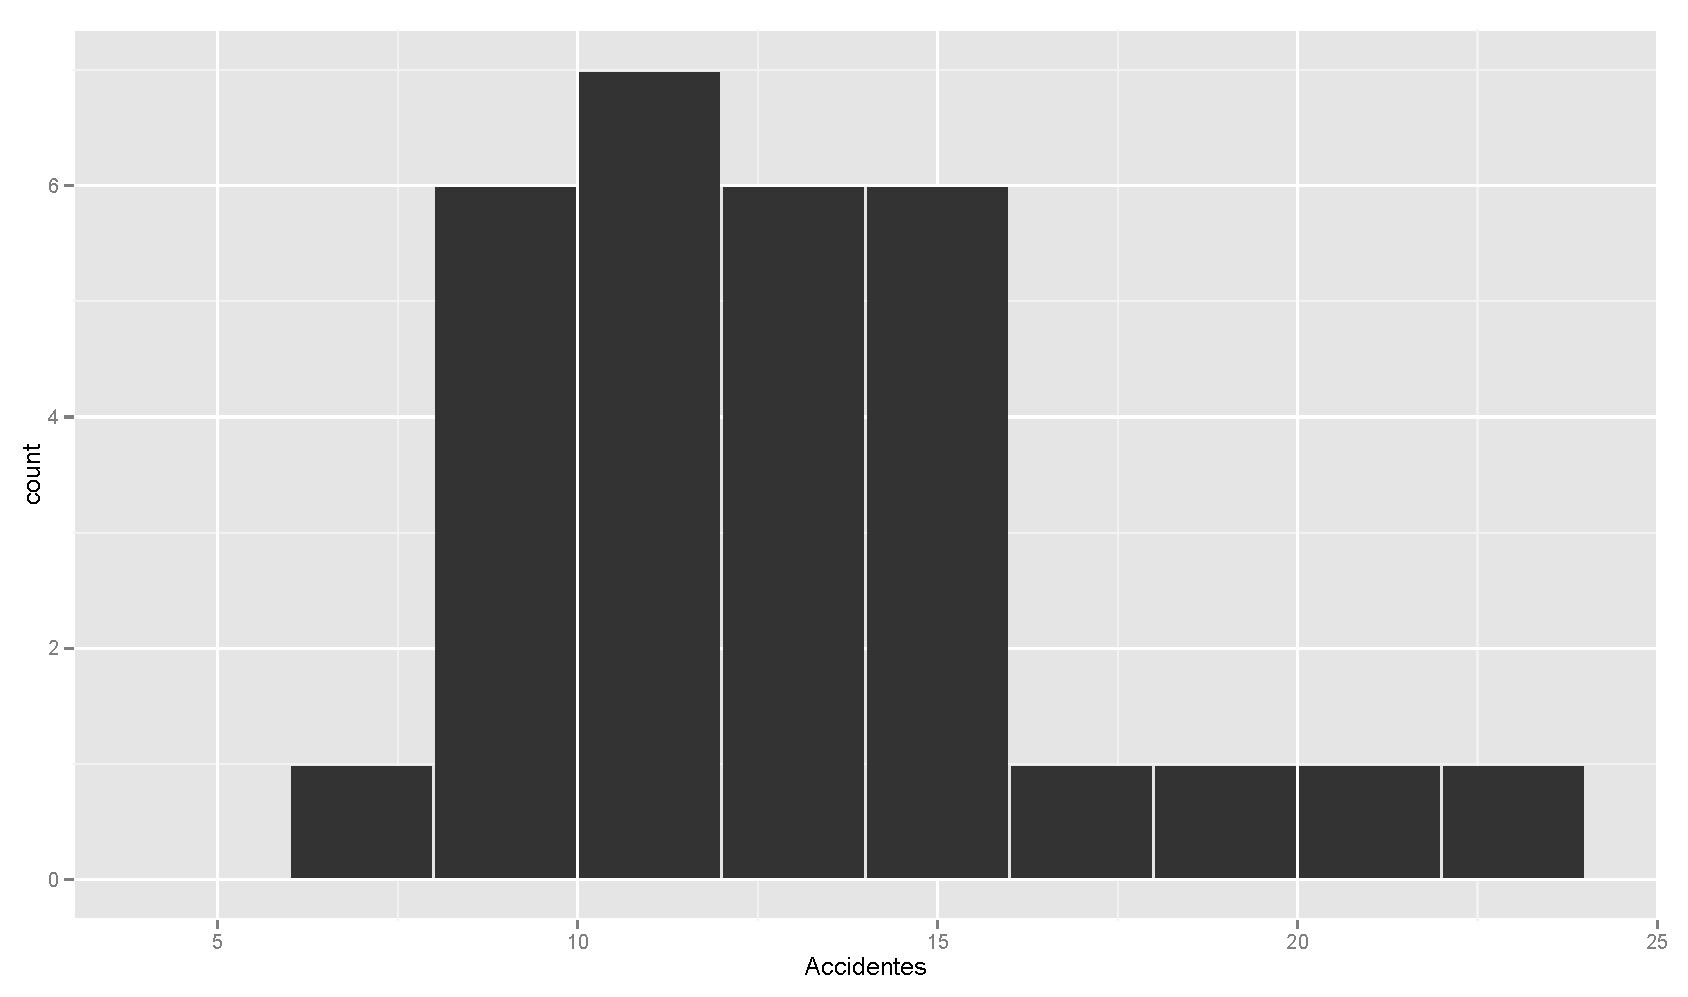
\includegraphics[scale=0.5]{EjemPoisson1.pdf}
    \caption{\emph{Histograma para los datos de accidentes de tr\'ansito.}}
    \label{EjemPoisson1}
    \end{figure}
    
    En primera instancia, es posible realizar un an\'alisis no informativo, al formular una distribuci\'on previa de Jeffreys, utilizando el resultado del ejemplo \ref{EjemPoisson1} de la p\'agina \pageref{EjemPoisson1}, que indica que una distribuci\'on previa no informativa es proporcional a $\theta^{-1/2}$, para lo cual la distribuci\'on posterior $Gamma(\sum_{i=1}^n y_i+1/2, n)$. De esta manera, la distribuci\'on posterior del par\'ametro de inter\'es es $Gamma(370.5, 30)$. Por lo tanto, un estimador de $\theta$ est\'a dado por la media de la distribuci\'on posterior que es $370.5/30=12.35$, muy cercano al valor del estimador de m\'axima verosimilitud correspondiente al promedio muestral. La figura \ref{EjemPoisson2} (lado izquierdo) muestra el comportamiento de las distribuciones de Jeffreys y posterior para este ejemplo.
    
    Por otro lado, bas\'andose en datos hist\'oricos, la alcald\'ia observ\'o que, en el mismo periodo del a\~no anterior, ocurrieron 37 accidentes en 9 d\'ias de observaci\'on. Luego, una distribuci\'on previa informativa\footnote{En la pr\'actica, se recomienda que los valores de los hiperpar\'ametros $\alpha$ y $\beta$ correspondan a la suma del n\'umero de eventos m\'as uno y n\'umero de observaciones, respectivamente.} est\'a dada por $Gamma(\alpha=38,\beta=9)$. Luego, apelando al resultado \ref{ResPoissonPost}, la distribuci\'on posterior corresponde a una $Gamma(370+38, 30+9)=Gamma(408, 39)$. Para este caso, un estimador de $\theta$ est\'a dado por la media de la distribuci\'on posterior que es $480/39=12.31$. La figura \ref{EjemPoisson2} (lado derecho) muestra el comportamiento de las distribuciones previa (informativa) y posterior para este ejemplo.
    
    \begin{figure}[!h]
    \centering
    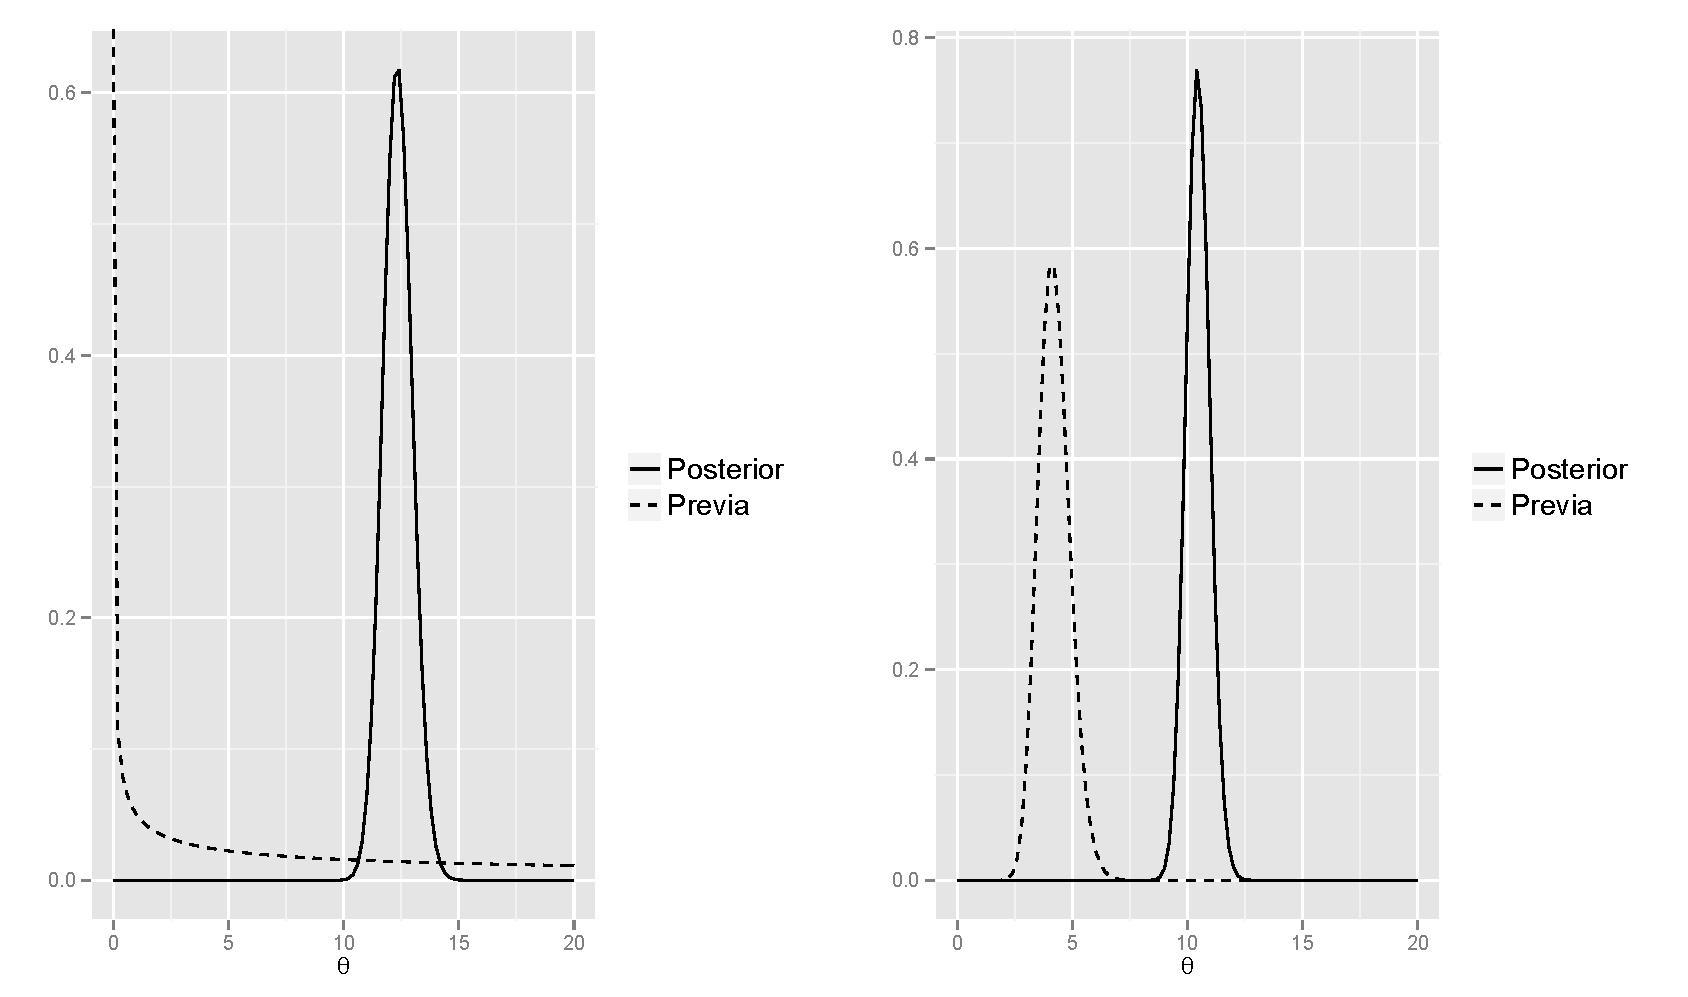
\includegraphics[width=18cm,height=8cm]{EjemPoisson2.pdf}
    \caption{\emph{Distribuci\'on previa y distribuci\'on posterior para el ejemplo del tr\'ansito con dos distribuciones previas diferentes (el lado izquierdo representa el caso cuando se usa la previa no informativa, el lado derecho la previa informativa).}}
    \label{EjemPoisson2}
    \end{figure}
    
    A continuaci\'on se examina la distribuci\'on predictiva. En la figura \ref{pred_post_pois} se grafica la distribuci\'on predictiva para una nueva observaci\'on cuando se usa la previa no informativa y la previa informativa. Los c\'odigos para el c\'alculo cuando se usa la previa no informativa es como siguen:
\begin{knitrout}
\definecolor{shadecolor}{rgb}{0.933, 0.933, 0.933}\color{fgcolor}\begin{kframe}
\begin{alltt}
\hlstd{Trans} \hlkwb{<-} \hlkwd{c}\hlstd{(}\hlnum{22}\hlstd{,} \hlnum{9}\hlstd{,} \hlnum{9}\hlstd{,} \hlnum{20}\hlstd{,} \hlnum{10}\hlstd{,} \hlnum{14}\hlstd{,} \hlnum{11}\hlstd{,} \hlnum{14}\hlstd{,} \hlnum{11}\hlstd{,} \hlnum{11}\hlstd{,} \hlnum{19}\hlstd{,} \hlnum{12}\hlstd{,} \hlnum{8}\hlstd{,} \hlnum{9}\hlstd{,} \hlnum{16}\hlstd{,} \hlnum{8}\hlstd{,} \hlnum{13}\hlstd{,} \hlnum{8}\hlstd{,} \hlnum{14}\hlstd{,} \hlnum{12}\hlstd{,}
\hlnum{14}\hlstd{,} \hlnum{11}\hlstd{,} \hlnum{14}\hlstd{,} \hlnum{13}\hlstd{,} \hlnum{11}\hlstd{,} \hlnum{14}\hlstd{,} \hlnum{13}\hlstd{,} \hlnum{11}\hlstd{,} \hlnum{7}\hlstd{,} \hlnum{12} \hlstd{)}
\hlstd{n} \hlkwb{<-} \hlkwd{length}\hlstd{(Trans)}
\hlstd{pre.Transito.NoInf} \hlkwb{<-} \hlkwa{function}\hlstd{(}\hlkwc{s}\hlstd{)\{}
\hlkwa{if}\hlstd{(s}\hlopt{>}\hlnum{0}\hlstd{)\{}
\hlstd{val} \hlkwb{<-} \hlkwd{gamma}\hlstd{(s)}\hlopt{*}\hlstd{(n}\hlopt{/}\hlstd{(n}\hlopt{+}\hlnum{1}\hlstd{))}\hlopt{^}\hlstd{(}\hlkwd{sum}\hlstd{(Trans)}\hlopt{+}\hlnum{0.5}\hlstd{)}\hlopt{/}
\hlstd{(}\hlkwd{beta}\hlstd{(s,}\hlkwd{sum}\hlstd{(Trans)}\hlopt{+}\hlnum{0.5}\hlstd{)}\hlopt{*}\hlkwd{prod}\hlstd{(}\hlnum{1}\hlopt{:}\hlstd{s)}\hlopt{*}\hlstd{(n}\hlopt{+}\hlnum{1}\hlstd{)}\hlopt{^}\hlstd{s)}
\hlstd{\}}
\hlkwa{if}\hlstd{(s}\hlopt{==}\hlnum{0}\hlstd{)\{}
\hlstd{val} \hlkwb{<-} \hlstd{(n}\hlopt{/}\hlstd{(n}\hlopt{+}\hlnum{1}\hlstd{))}\hlopt{^}\hlstd{(}\hlkwd{sum}\hlstd{(Trans)}\hlopt{+}\hlnum{0.5}\hlstd{)}
\hlstd{\}}
\hlstd{val}
\hlstd{\}}
\hlstd{s.max} \hlkwb{<-} \hlnum{40}\hlstd{; s.val} \hlkwb{<-} \hlnum{0}\hlopt{:}\hlstd{s.max; pre.NoInf.val} \hlkwb{<-} \hlkwd{c}\hlstd{()}
\hlkwa{for}\hlstd{(i} \hlkwa{in} \hlnum{1}\hlopt{:}\hlkwd{length}\hlstd{(s.val))\{}
\hlstd{pre.NoInf.val[i]} \hlkwb{<-} \hlkwd{pre.Transito.NoInf}\hlstd{(s.val[i])}
\hlstd{\}}
\hlkwd{sum}\hlstd{(pre.NoInf.val)}
\end{alltt}
\begin{verbatim}
## [1] 1
\end{verbatim}
\end{kframe}
\end{knitrout}
    N\'otese que en los anteriores c\'odigos, se us\'o como valor m\'aximo de 40 para la variable $\mathbf{\tilde{s}}$ a pesar de que \'esta toma valores infinitos, pero al ver que la suma de las probabilidades desde el valor 0 hasta el m\'aximo de 40 es igual a 1, podemos concluir que la probabilidad de que $\mathbf{\tilde{s}}$ tome valores mayores a 40 es pr\'acticamente nula.
    
    Finalmente, podemos tener una aproximaci\'on de la esperanza de la variable $\mathbf{\tilde{s}}$ como
\begin{knitrout}
\definecolor{shadecolor}{rgb}{0.933, 0.933, 0.933}\color{fgcolor}\begin{kframe}
\begin{alltt}
\hlkwd{sum}\hlstd{(pre.NoInf.val}\hlopt{*}\hlstd{s.val)}
\end{alltt}
\begin{verbatim}
## [1] 12.35
\end{verbatim}
\end{kframe}
\end{knitrout}
    
    \begin{figure}[!h]
    \centering
    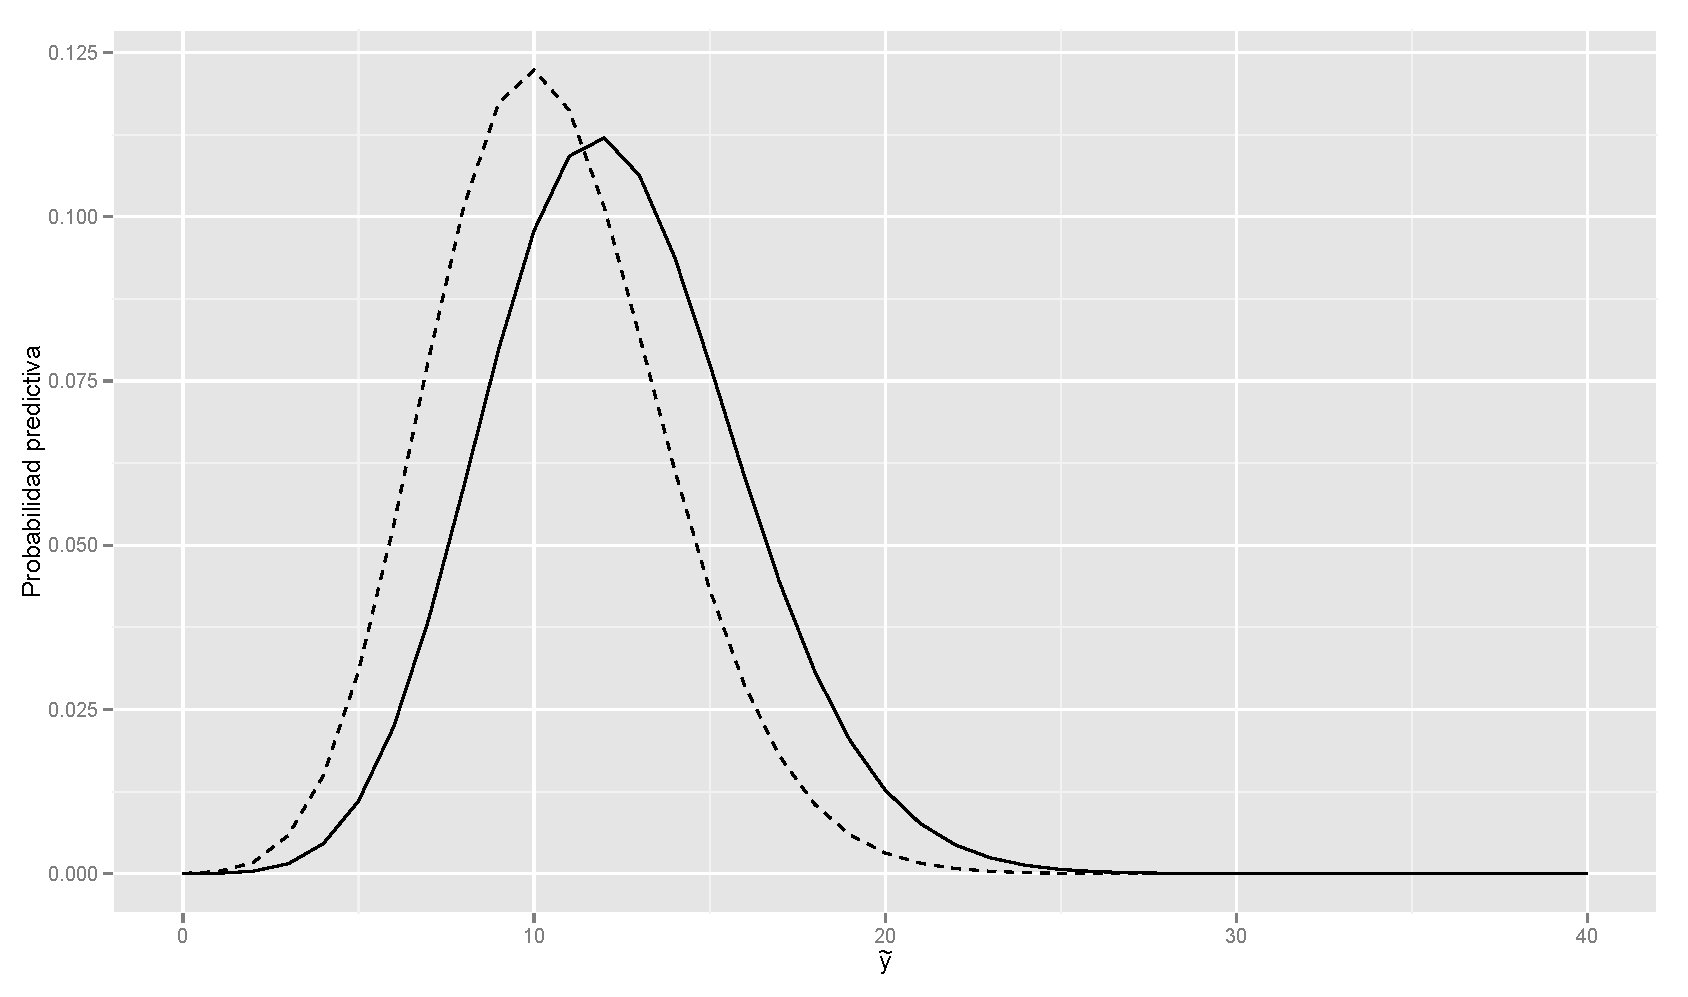
\includegraphics[scale=0.4]{predpostpois.pdf}
    \caption{\emph{Distribuci\'on predictiva posterior para $n*=1$ para el ejemplo del tr\'ansito. La l\'inea s\'olida denota la distribuci\'on predictiva obtenida con la previa no informativa, la l\'inea continua denota la obtenida con la previa $Gamma(\alpha=38,\beta=9)$.}}
    \label{pred_post_pois}
    \end{figure}
    
    \end{Eje}
    
    \section{Modelo exponencial}
    
    Suponga que $\mathbf{Y}=\{Y_1,\ldots,Y_n\}$ corresponde a una muestra de variables aleatorias con distribuci\'on Exponencial. Luego, la funci\'on de distribuci\'on conjunta o verosimilitud est\'a dada por
    
    \begin{align}
    p(\mathbf{Y} \mid \theta)&=\prod_{i=1}^n\theta e^{(-\theta y)}I_{(0,\infty)}(y_i) \notag \\
    &=\theta^n e^{(-\theta \sum_{i=1}^ny_i)}I_{(0,\infty)^n}(y_1,\ldots,y_n)
    \end{align}
    
    Donde $\{0,1\ldots\}^n$ denota el producto cartesiano $n$ veces sobre el intervalo $(0,\infty)$. Por otro lado, como el par\'ametro $\theta$ est\'a restringido al espacio $\Theta=(0,\infty)$, entonces es posible formular varias opciones para la distribuci\'on previa del par\'ametro, al igual que en la distribuci\'on Poisson. As\'i mismo, suponga que la distribuci\'on previa para el par\'ametro de inter\'es es la distribuci\'on Gamma tal como aparece en la expresi\'on (2.1.9). Bajo este marco de referencia se tienen los siguientes resultados
    
    \begin{Res}
    La distribuci\'on posterior del par\'ametro $\theta$ sigue una distribuci\'on
    \begin{equation*}
    \theta \mid \mathbf{Y} \sim Gamma\left(\alpha+n,\beta+\sum_{i=1}^ny_i\right)
    \end{equation*}
    \end{Res}
    
    \begin{proof}
    \begin{align*}
    p(\theta \mid \mathbf{Y})&\propto p(\mathbf{Y} \mid \theta)p(\theta \mid \alpha,\beta)\\
    &=\theta^n e^{(-\theta \sum_{i=1}^ny_i)}I_{(0,\infty)^n}(y_1,\ldots,y_n)\frac{\beta^\alpha \theta^{\alpha-1} e^{-\beta\theta}}{\Gamma(\alpha)}I_{(0,\infty)}(\theta)\\
    &\propto \theta^{\alpha+n-1}e^{-(\beta+\sum_{i=1}^ny_i)}I_{(0,\infty)}(\theta)
    \end{align*}
    Por lo tanto, factorizando convenientemente, se encuentra una expresi\'on id\'entica a la funci\'on de distribuci\'on de una variable aleatoria con distribuci\'on $Gamma(\alpha+n,\beta+\sum_{i=1}^ny_i)$.
    \end{proof}
    
    \begin{Res}
    La distribuci\'on predictiva previa para una observaci\'on $\mathbf{y}=\{y_1,\ldots,y_n\}$ de la muestra aleatoria est\'a dada por
    \begin{equation}
    p(\mathbf{Y})=\frac{\Gamma(\alpha+n)}{\Gamma(\alpha)}\frac{\beta^\alpha}{(\beta+\sum_{i=1}^ny_i)^{\alpha+n}}
    I_{(0,\infty)^n}(y_1,\ldots,y_n)
    \end{equation}
    y define una aut\'entica funci\'on de densidad de probabilidad continua.
    \end{Res}
    
    \begin{proof}
    De la definici\'on de funci\'on de distribuci\'on predictiva se tiene que
    \begin{align*}
    p(\mathbf{Y})&=\int p(\mathbf{Y} \mid \theta)p(\theta \mid \alpha,\beta)\ d\theta\\
    &=\int_0^{\infty}\theta^n e^{(-\theta \sum_{i=1}^ny_i)}I_{(0,\infty)^n}(y_1,\ldots,y_n)\frac{\beta^\alpha \theta^{\alpha-1} e^{-\beta\theta}}{\Gamma(\alpha)} \ d\theta\\
    &=\frac{\Gamma(n+\alpha)}{\Gamma(\alpha)}\frac{\beta^\alpha}{(\beta+\sum_{i=1}^ny_i)^{\alpha+n}}I_{(0,\infty)^n}(y_1,\ldots,y_n)\\
    &\hspace{2cm}\times
    \int_0^{\infty} \frac{(\beta+\sum_{i=1}^ny_i)^{\alpha+n}}{\Gamma(n+\alpha)} \theta^{\alpha+n-1}e^{-(\beta+\sum_{i=1}^ny_i)\theta}
    \ d\theta\\
    &=\frac{\Gamma(\alpha+n)}{\Gamma(\alpha)}\frac{\beta^\alpha}{(\beta+\sum_{i=1}^ny_i)^{\alpha+n}}I_{(0,\infty)^n}(y_1,\ldots,y_n)
    \end{align*}
    \end{proof}
    
    Por ejemplo, en el caso en que la muestra aleatoria estuviera constituida por una sola variable aleatoria, entonces no es dif\'icil ver, utilizando la definici\'on de la funci\'on matem\'atica Gamma, que la funci\'on de distribuci\'on predictiva (2.2.2) estar\'ia dada por
    \begin{align*}
    p(Y)&=\frac{\Gamma(\alpha+1)}{\Gamma(\alpha)}\frac{\beta^\alpha}{(\beta+y)^{\alpha+1}}
    I_{(0,\infty)}(y)\notag \\
    &=\frac{\alpha \beta^\alpha}{(\beta+y)^{\alpha+1}}
    I_{(0,\infty)}(y)
    \end{align*}
    
    Para chequear la convergencia de la anterior distribuci\'on es necesario recurrir a los resultados del c\'alculo integral. Dado que el espacio de muestreo de la variable aleatoria $Y$ es el intervalo $(0,\infty)$, entonces la integral a uno lo que conlleva a que, en este caso particular, $P(Y)$ sea una aut\'entica funci\'on de densidad de probabilidad.
    \begin{align*}
    \int_0^{\infty}p(Y)\ dy=\int_0^{\infty}\frac{\alpha \beta^\alpha}{(\beta+y)^{\alpha+1}} \ dy
    =  \beta^\alpha \left[\frac{(\beta+y)^{-\alpha}}{-\alpha} \right]_0^{\infty}
    =1
    \end{align*}
    
    Volviendo al caso general en donde se tiene una muestra aleatoria, se tiene el siguiente resultado.
    
    \begin{Res}
    Despu\'es de la recolecci\'on de los datos, la distribuci\'on predictiva posterior para una conjunto de nuevas variables aleatorias $\tilde{\mathbf{y}}=\{\tilde{y}_1,\ldots,\tilde{y}_{n^*}\}$, de tama\~no $n^*$, est\'a dada por
    \begin{align}
    p(\tilde{\mathbf{y}} \mid \mathbf{Y})&=
    \frac{\Gamma(n+\alpha+n^{*})}{\Gamma(n+\alpha)}
    \frac{(\beta+\sum_{i=1}^ny_i)^{n+\alpha}}{(\sum_{i=1}^{n^*}\tilde{y}_i+\beta+\sum_{i=1}^ny_i)^{n^*+\alpha+n}}\notag\\
    &\hspace{4cm}\times
    I_{(0,\infty)^{n^*}}(\tilde{y}_1,\ldots,\tilde{y}_n)
    \end{align}
    \end{Res}
    
    \begin{proof}
    De la definici\'on de funci\'on de distribuci\'on predictiva, y haciendo uso del mismo razonamiento en la demostraci\'on del Resultado 2.2.2, se tiene la prueba inmediatamente.
    \end{proof}
    
    El anterior resultado permite calcular la distribuci\'on predictiva conjunta de variables aleatorias por observar, en algunas situaciones, lo que se quiere pronosticar es el comportamiento probabil\'istico de promedio muestral de este conjunto de variables aleatorias, es decir, $\bar{Y}^*=\sum_{i=1}^{n^*}\tilde{Y}_i$. En el siguiente resultado se presenta la distribuci\'on predictiva de esta variable aleatoria.
    \begin{Res}
    Despu\'es de la recolecci\'on de los datos, la distribuci\'on predictiva posterior para el promedio muestral de un nuevo conjunto de variables aleatorias $\bar{Y}^*=\sum_{i=1}^{n^*}\tilde{Y}_i$ est\'a dada por
    \begin{equation*}
    p(\bar{Y}^*)=\frac{n^*\Gamma(n^*+\alpha+n)}{\Gamma(n^*)\Gamma(\alpha+n)}\frac{(\beta+\sum_{i=1}^ny_i)^{\alpha+n}}{(n^*\bar{Y}^*+\beta+\sum y_i)^{n^*+\alpha+n}}(n^*\bar{Y}^*)^{n^*-1}I_{(0,\infty)}(\bar{Y}^*)
    \end{equation*}
    \end{Res}
    
    \begin{proof}
    En primer lugar se halla la distribuci\'on predictiva posterior de la variable $\tilde{S}=\sum_{i=1}^{n^*}\tilde{Y}_i$, teniendo en cuenta que $\tilde{S}|\theta\sim Gamma(n^*,\theta)$, de esta forma
    \begin{align*}
    p(\tilde{S}|\mathbf{Y})&=\int p(\tilde{S}|\theta)p(\theta|\mathbf{Y})\ d\theta\\
    &=\int_0^{\infty} \frac{\theta^{n^*}}{\Gamma(n^*)}\tilde{S}^{n^*-1}e^{-\theta\tilde{S}}I_{(0,\infty)}(\tilde{S})\frac{(\beta+\sum_{i=1}^ny_i)^{\alpha+n}}{\Gamma(\alpha+n)}\theta^{{\alpha+n-1}}e^{-(\beta+\sum y_i)\theta}d\theta\\
    &=\frac{\tilde{S}^{n^*-1}(\beta+\sum_{i=1}^ny_i)^{\alpha+n}}{\Gamma(n^*)\Gamma(\alpha+n)}I_{(0,\infty)}(\tilde{S})\int_0^{\infty} \theta^{n^*+\alpha+n-1}e^{-(\tilde{S}+\beta+\sum y_i)\theta}\ d\theta\\
    &=\frac{\tilde{S}^{n^*-1}(\beta+\sum_{i=1}^ny_i)^{\alpha+n}}{\Gamma(n^*)\Gamma(\alpha+n)}\frac{\Gamma(n^*+\alpha+n)}{(\tilde{S}+\beta+\sum y_i)^{n^*+\alpha+n}}I_{(0,\infty)}(\tilde{S})
    \end{align*}
    Al aplicar el teorema de transformaci\'on a la distribuci\'on predictiva, se puede hallar la distribuci\'on de $\bar{Y}^*$, dada por
    \begin{align*}
    p(\bar{Y}^*|\mathbf{Y})=\frac{n^*\Gamma(n^*+\alpha+n)}{\Gamma(n^*)\Gamma(\alpha+n)}\frac{(\beta+\sum_{i=1}^ny_i)^{\alpha+n}}{(n^*\bar{Y}^*+\beta+\sum y_i)^{n^*+\alpha+n}}(n^*\bar{Y}^*)^{n^*-1}I_{(0,\infty)}(\bar{Y}^*)
    \end{align*}
    \end{proof}
    
    En la pr\'actica puede ocurrir que alguos de los valores de $n$, $n^*$, $\sum_{i=1}^ny_i$ y $n^*\bar{Y}^*$ son muy grandes, y evaluar directamente la expresi\'on anterior puede ocasionar problemas num\'ericos. Realizando algunas operaciones algebr\'aicas, se encuentra la siguiente expresi\'on equivalente para la distribuci\'on predictiva posterior de $\bar{Y}^*$ que evita problemas num\'ericas:
    \begin{equation}\label{pred_expo_Informa2}
    p(\bar{Y}^*|\mathbf{Y})=\frac{1}{\bar{Y}^*Beta(n,n^*)}\left(\frac{\beta+\sum_{i=1}^ny_i}{\beta+\sum_{i=1}^ny_i+n^*\bar{Y}^*}\right)^{\alpha+n}\left(\frac{n^*\bar{Y}^*}{\beta+\sum_{i=1}^ny_i+n^*\bar{Y}^*}\right)^{n^*}I_{(0,\infty)}(\bar{Y}^*)
    \end{equation}
    
    Por otro lado, se puede ver que al utilizar la distribuci\'on previa no informativa de Jeffrey, la distribuci\'on predictiva posterior de $\bar{Y}^*$ est\'a dada por
    \begin{equation}\label{pred_expo_Jeffreys1}
    p(\bar{Y}^*|\mathbf{Y})=\frac{n^*\Gamma(n^*+n)}{\Gamma(n^*)\Gamma(n)}\frac{(\sum_{i=1}^ny_i)^n}{(n^*\bar{Y}^*+\sum y_i)^{n^*+n}}(n^*\bar{Y}^*)^{n^*-1}I_{(0,\infty)}(\bar{Y}^*)
    \end{equation}
    La cual es equivalente a la siguiente expresi\'on que en ocasiones puede ser \'util para evitar problemas num\'ericos
    
    \begin{equation}\label{pred_expo_Jeffreys2}
    p(\bar{Y}^*|\mathbf{Y})=\frac{1}{\bar{Y}^*Beta(n,n^*)}\left(\frac{\sum_{i=1}^ny_i}{\sum_{i=1}^ny_i+n^*\bar{Y}^*}\right)^n\left(\frac{n^*\bar{Y}^*}{\sum_{i=1}^ny_i+n^*\bar{Y}^*}\right)^{n^*}I_{(0,\infty)}(\bar{Y}^*)
    \end{equation}
    
    \begin{Eje}
    \citeasnoun{survi} reportan un conjunto de datos que da cuenta de los tiempos de sobrevivencia de $n=69$ miembros del programa de transplante de coraz\'on de Stanford.Los tiempos se reportan en d\'ias despu\'es del transplante. Los datos pueden ser encontrados en el paquete \verb'survival' \cite{survival} de \verb'R' mediante la implementaci\'on del siguiente c\'odigo computacional.
    
    \colorbox{black}{\textcolor{white}{\textbf{C\'odigo R}}}
\begin{knitrout}
\definecolor{shadecolor}{rgb}{0.933, 0.933, 0.933}\color{fgcolor}\begin{kframe}
\begin{alltt}
\hlkwd{require}\hlstd{(survival)}
\hlkwd{data}\hlstd{(heart)}
\hlkwd{attach}\hlstd{(heart)}
\end{alltt}


{\ttfamily\noindent\itshape\color{messagecolor}{\#\# The following object is masked from package:survival:\\\#\# \\\#\#\ \ \ \  transplant}}\begin{alltt}
\hlkwd{View}\hlstd{(heart)}
\end{alltt}


{\ttfamily\noindent\color{warningcolor}{\#\# Warning: running command ''/usr/bin/otool' -L '/Library/Frameworks/R.framework/Resources/modules/R\_de.so'' had status 1}}

{\ttfamily\noindent\color{warningcolor}{\#\# Warning in View(heart): unable to load shared object '/Library/Frameworks/R.framework/Resources/modules//R\_de.so':\\\#\#\ \  dlopen(/Library/Frameworks/R.framework/Resources/modules//R\_de.so, 6): Library not loaded: /opt/X11/lib/libSM.6.dylib\\\#\#\ \  Referenced from: /Library/Frameworks/R.framework/Resources/modules//R\_de.so\\\#\#\ \  Reason: image not found}}

{\ttfamily\noindent\bfseries\color{errorcolor}{\#\# Error in View(heart): X11 dataentry cannot be loaded}}\begin{alltt}
\hlstd{sobrevida} \hlkwb{<-} \hlstd{stop[transplant}\hlopt{==}\hlnum{1}\hlstd{]} \hlopt{-} \hlstd{start[transplant}\hlopt{==}\hlnum{1}\hlstd{]}
\hlkwd{data.frame}\hlstd{(heart[transplant}\hlopt{==}\hlnum{1}\hlstd{,], sobrevida)}
\end{alltt}
\begin{verbatim}
##     start stop event       age   year surgery transplant  id sobrevida
## 4     1.0   16     1   6.29706 0.2656       0          1   3      15.0
## 6    36.0   39     1  -7.73717 0.4901       0          1   4       3.0
## 10   51.0  675     1   2.86927 0.7803       0          1   7     624.0
## 14   12.0   58     1  -5.49760 0.8624       0          1  10      46.0
## 16   26.0  153     1  -0.01916 0.8734       0          1  11     127.0
## 19   17.0   81     1   6.57358 0.9692       0          1  13      64.0
## 21   37.0 1387     1   6.01232 0.9719       0          1  14    1350.0
## 24   28.0  308     1   1.44832 1.0705       0          1  16     280.0
## 27   20.0   43     1   8.84873 1.0869       0          1  18      23.0
## 30   18.0   28     1   7.27995 1.3306       0          1  20      10.0
## 32    8.0 1032     1  -4.65708 1.3388       0          1  21    1024.0
## 34   12.0   51     1  -5.21561 1.4620       0          1  22      39.0
## 36    3.0  733     1  10.35729 1.5277       0          1  23     730.0
## 38   83.0  219     1   3.80014 1.5661       0          1  24     136.0
## 40   25.0 1800     0 -14.77618 1.5743       0          1  25    1775.0
## 44   71.0   72     1   6.02327 1.6838       0          1  28       1.0
## 47   16.0  852     1  -3.08830 1.8836       0          1  30     836.0
## 50   17.0   77     1  16.40794 1.9110       0          1  32      60.0
## 52   51.0 1587     0   0.90349 2.1574       0          1  33    1536.0
## 54   23.0 1572     0  -7.44695 2.1985       0          1  34    1549.0
## 57   46.0  100     1   0.92539 2.5079       0          1  36      54.0
## 59   19.0   66     1  13.50034 2.5654       0          1  37      47.0
## 61    4.5    5     1  -6.52977 2.5927       0          1  38       0.5
## 63    2.0   53     1   2.51882 2.6338       0          1  39      51.0
## 65   41.0 1408     0   0.48186 2.6475       1          1  40    1367.0
## 67   58.0 1322     0  -2.69678 2.8830       1          1  41    1264.0
## 72    1.0   45     1 -11.81656 3.2635       0          1  45      44.0
## 74    2.0  996     1   0.61054 3.2772       1          1  46     994.0
## 76   21.0   72     1  -0.90075 3.3402       0          1  47      51.0
## 79   36.0 1142     0 -11.34565 3.3758       1          1  49    1106.0
## 81   83.0  980     1  -2.11362 3.3758       1          1  50     897.0
## 83   32.0  285     1   0.73374 3.4771       0          1  51     253.0
## 86   41.0  188     1  -0.65708 3.7509       0          1  53     147.0
## 89   10.0   61     1   4.45448 3.8549       0          1  55      51.0
## 91   67.0  942     0  -9.25667 3.9233       0          1  56     875.0
## 94   21.0  343     1   0.01643 3.9781       1          1  58     322.0
## 96   78.0  916     0  -6.61739 3.9945       1          1  59     838.0
## 98    3.0   68     1   1.05407 4.1314       0          1  60      65.0
## 102  27.0  842     0 -15.34018 4.1971       0          1  63     815.0
## 104  33.0  584     1   0.81588 4.3368       1          1  64     551.0
## 106  12.0   78     1   3.29363 4.4298       0          1  65      66.0
## 109  57.0  285     1 -28.44901 4.4764       0          1  67     228.0
## 111   3.0   68     1  -2.75975 4.5175       0          1  68      65.0
## 113  10.0  670     0  -0.01095 4.6680       0          1  69     660.0
## 115   5.0   30     1   5.00205 4.7118       0          1  70      25.0
## 117  31.0  620     0  -0.59138 4.8049       0          1  71     589.0
## 119   4.0  596     0 -21.27310 4.8706       0          1  72     592.0
## 121  27.0   90     1   8.33128 4.9473       0          1  73      63.0
## 123   5.0   17     1 -18.83368 4.9665       0          1  74      12.0
## 126  46.0  545     0   4.08487 5.0103       1          1  76     499.0
## 129 210.0  515     0   0.70363 5.0924       0          1  78     305.0
## 131  67.0   96     1   5.78234 5.1663       0          1  79      29.0
## 133  26.0  482     0  -1.55510 5.1828       1          1  80     456.0
## 135   6.0  445     0   4.89254 5.2841       0          1  81     439.0
## 138  32.0   80     1   5.30869 5.3169       0          1  83      48.0
## 140  37.0  334     1  -5.28131 5.3333       0          1  84     297.0
## 143   8.0  397     0   0.91992 5.4155       0          1  86     389.0
## 145  60.0  110     1  -1.74675 5.4702       0          1  87      50.0
## 147  31.0  370     0   6.36277 5.4894       0          1  88     339.0
## 149 139.0  207     1   3.04723 5.5113       0          1  89      68.0
## 151 160.0  186     1   4.03285 5.5140       1          1  90      26.0
## 154 310.0  340     0  -3.01711 5.5715       0          1  92      30.0
## 156  28.0  265     0  -0.24914 5.7769       0          1  93     237.0
## 158   4.0  165     1  -4.15880 5.9548       1          1  94     161.0
## 160   2.0   16     1  -7.71800 5.9767       0          1  95      14.0
## 162  13.0  180     0 -21.34976 6.0096       0          1  96     167.0
## 164  21.0  131     0 -24.38330 6.1437       0          1  97     110.0
## 166  96.0  109     0 -19.37029 6.2040       0          1  98      13.0
## 169  38.0   39     0 -12.93908 6.3956       1          1 100       1.0
\end{verbatim}
\end{kframe}
\end{knitrout}
    
    A continuaci\'on se muestran los primeros y \'ultimos datos de este estudio. Se recuerda que el total de pacientes atendidos en este estudio fue de $n=69$ y la suma de los tiempos de sobrevida es de $\sum_{i=1}^ny_i=25998.5$.
    
    \begin{verbatim}
    id      start     stop     Sobrevida
    
    3        1.0       16          15.0
    4       36.0       39           3.0
    7       51.0      675         624.0
    
    ...        ...      ...           ...
    
    97       21.0      131         110.0
    98       96.0      109          13.0
    100       38.0       39           1.0
    \end{verbatim}
    
    Estos tiempos pueden ser modelados mediante una distribuci\'on exponencial. Adem\'as de inferir acerca del par\'ametro de esta distribuci\'on, tambi\'en es posible inferir acerca del tiempo promedio de sobrevivencia de un individuo sometido a este tipo de transplantes. Luego, dadas las implicaciones del estudio, se debe ser muy cuidadosos en la asignaci\'on de los par\'ametros de la distribuci\'on previa. Una forma de hacerlo es asignar valores muy peque\~nos a estos par\'ametros. Otra forma de hacerlo es utilizando la distribuci\'on previa de Jeffreys, que corresponde a una distribuci\'on impropia (ver ejercicio XXXXXXXXXX) y conduce a resultados muy cercanos a los del enfoque anterior.
    
    Utilizando par\'ametros previos muy cercanos a cero, la distribuci\'on posterior del par\'ametro de inter\'es es $Gamma(69, 25998.5)$. Como es bien sabido, una estimaci\'on bayesiana para el par\'ametro $\theta$ est\'a dada por la media de esta distribuci\'on posterior, la cual equivale a $69/25998.5=0.0026$. Ahora, como la esperanza de la distribuci\'on exponencial es $1/\theta$, entonces el tiempo promedio de sobrevivencia es de $1/0.0026=376.78$ d\'ias. Sin embargo, el promedio no es una medida de escala v\'alidas en este tipo de an\'alisis, en donde se presentan datos at\'ipicos, puesto que no es una medida robusta y se prefiere la utilizaci\'on de la mediana. El siguiente c\'odigo computacional en JAGS puede ser usado para realizar inferencias sobre el par\'ametro $\theta$, sobre el tiempo promedio y el tiempo mediano. De la misma forma, es posible obtener intervalos de credibilidad para estos par\'ametros.
    
    \colorbox{black}{\textcolor{white}{\textbf{C\'odigo JAGS}}}
\begin{knitrout}
\definecolor{shadecolor}{rgb}{0.933, 0.933, 0.933}\color{fgcolor}\begin{kframe}
\begin{alltt}
\hlstd{Exp.model} \hlkwb{<-} \hlkwa{function}\hlstd{()\{}
\hlkwa{for}\hlstd{(i} \hlkwa{in} \hlnum{1}\hlopt{:}\hlstd{n)}
\hlstd{\{}
\hlstd{y[i]} \hlopt{~} \hlkwd{dexp}\hlstd{(theta)}
\hlstd{\}}
\hlstd{theta} \hlopt{~} \hlkwd{dgamma}\hlstd{(}\hlnum{0.1}\hlstd{,}\hlnum{0.1}\hlstd{)}
\hlstd{mean} \hlkwb{<-} \hlnum{1}\hlopt{/}\hlstd{theta}
\hlstd{\}}

\hlstd{n} \hlkwb{<-}\hlnum{69}
\hlstd{y} \hlkwb{<-} \hlkwd{c}\hlstd{(}\hlnum{15}\hlstd{,} \hlnum{3}\hlstd{,} \hlnum{624}\hlstd{,} \hlnum{46}\hlstd{,} \hlnum{127}\hlstd{,} \hlnum{64}\hlstd{,} \hlnum{1350}\hlstd{,} \hlnum{280}\hlstd{,} \hlnum{23}\hlstd{,} \hlnum{10}\hlstd{,} \hlnum{1024}\hlstd{,} \hlnum{39}\hlstd{,} \hlnum{730}\hlstd{,} \hlnum{136}\hlstd{,} \hlnum{1775}\hlstd{,} \hlnum{1}\hlstd{,} \hlnum{836}\hlstd{,} \hlnum{60}\hlstd{,} \hlnum{1536}\hlstd{,} \hlnum{1549}\hlstd{,} \hlnum{54}\hlstd{,} \hlnum{47}\hlstd{,} \hlnum{0.5}\hlstd{,} \hlnum{51}\hlstd{,} \hlnum{1367}\hlstd{,} \hlnum{1264}\hlstd{,} \hlnum{44}\hlstd{,} \hlnum{994}\hlstd{,} \hlnum{51}\hlstd{,} \hlnum{1106}\hlstd{,} \hlnum{897}\hlstd{,} \hlnum{253}\hlstd{,} \hlnum{147}\hlstd{,} \hlnum{51}\hlstd{,} \hlnum{875}\hlstd{,} \hlnum{322}\hlstd{,} \hlnum{838}\hlstd{,} \hlnum{65}\hlstd{,} \hlnum{815}\hlstd{,} \hlnum{551}\hlstd{,} \hlnum{66}\hlstd{,} \hlnum{228}\hlstd{,} \hlnum{65}\hlstd{,} \hlnum{660}\hlstd{,} \hlnum{25}\hlstd{,} \hlnum{589}\hlstd{,} \hlnum{592}\hlstd{,} \hlnum{63}\hlstd{,} \hlnum{12}\hlstd{,} \hlnum{499}\hlstd{,} \hlnum{305}\hlstd{,} \hlnum{29}\hlstd{,} \hlnum{456}\hlstd{,} \hlnum{439}\hlstd{,} \hlnum{48}\hlstd{,} \hlnum{297}\hlstd{,} \hlnum{389}\hlstd{,} \hlnum{50}\hlstd{,} \hlnum{339}\hlstd{,} \hlnum{68}\hlstd{,} \hlnum{26}\hlstd{,} \hlnum{30}\hlstd{,} \hlnum{237}\hlstd{,} \hlnum{161}\hlstd{,} \hlnum{14}\hlstd{,} \hlnum{167}\hlstd{,} \hlnum{110}\hlstd{,} \hlnum{13}\hlstd{,} \hlnum{1}\hlstd{)}

\hlstd{Exp.data} \hlkwb{<-} \hlkwd{list}\hlstd{(}\hlstr{"n"}\hlstd{,} \hlstr{"y"}\hlstd{)}
\hlstd{Exp.param} \hlkwb{<-} \hlkwd{c}\hlstd{(}\hlstr{"theta"}\hlstd{)}
\hlstd{Exp.inits} \hlkwb{<-} \hlkwa{function}\hlstd{()\{}
\hlkwd{list}\hlstd{(}\hlstr{"theta"}\hlstd{=}\hlnum{0.5}\hlstd{)}
\hlstd{\}}

\hlstd{Exp.fit} \hlkwb{<-} \hlkwd{jags}\hlstd{(}\hlkwc{data}\hlstd{=Exp.data,} \hlkwc{inits}\hlstd{=Exp.inits, Exp.param,} \hlkwc{n.iter}\hlstd{=}\hlnum{10000}\hlstd{,} \hlkwc{n.burnin}\hlstd{=}\hlnum{1000}\hlstd{,} \hlkwc{model.file}\hlstd{=Exp.model)}
\end{alltt}
\begin{verbatim}
## Compiling model graph
##    Resolving undeclared variables
##    Allocating nodes
## Graph information:
##    Observed stochastic nodes: 69
##    Unobserved stochastic nodes: 1
##    Total graph size: 76
## 
## Initializing model
\end{verbatim}
\begin{alltt}
\hlkwd{print}\hlstd{(Exp.fit)}
\end{alltt}
\begin{verbatim}
## Inference for Bugs model at "/var/folders/n7/01szs8_x7pq1bvpwwnvq7w_w0000gn/T//RtmpMtD1jH/model11b72d37702.txt", fit using jags,
##  3 chains, each with 10000 iterations (first 1000 discarded), n.thin = 9
##  n.sims = 3000 iterations saved
##          mu.vect sd.vect    2.5%     25%     50%     75%   97.5%  Rhat
## theta      0.003   0.000   0.002   0.002   0.003   0.003   0.003 1.001
## deviance 957.575   1.441 956.574 956.677 957.027 957.896 961.756 1.001
##          n.eff
## theta     2800
## deviance  3000
## 
## For each parameter, n.eff is a crude measure of effective sample size,
## and Rhat is the potential scale reduction factor (at convergence, Rhat=1).
## 
## DIC info (using the rule, pD = var(deviance)/2)
## pD = 1.0 and DIC = 958.6
## DIC is an estimate of expected predictive error (lower deviance is better).
\end{verbatim}
\end{kframe}
\end{knitrout}
    
    Despu\'es de diez mil iteraciones, los resultados de este c\'odigo muestran una estimaci\'on para	 $\theta$ de 0.0026 con un intervalo de credibilidad de (0.002065, 0.00332). Para la media $1/\theta$, se tiene una estimaci\'on puntual de 382.1 con un intervalo de credibilidad de (301.2, 484.3). La mediana se estim\'o en 378 d\'ias de sobrevivencia.
    
    Suponga ahora se va a realizar el transplante de coraz\'on a 5 pacientes, y se quiere conocer el comportamiento probabil\'istico del tiempo promedio de sobrevida en estos 5 pacientes. Aplicando la distribuci\'on predictiva obtenida en el resultado 2.5.4, usando la distribuci\'on previa no informativa de Jeffrey, se tiene que
    \begin{align*}
    p(\bar{Y}^*|\mathbf{Y})&=\frac{5\Gamma(5+69)}{\Gamma(5)\Gamma(69)}\frac{25998.5^{69}}{(5\bar{Y}^*+25998.5)^{5+69}}(5\bar{Y}^*)^4\\
    &=\frac{1}{\bar{Y}^*Beta(5,69)}\left(\frac{25998.5}{5\bar{Y}^*+25998.5}\right)^{69}\left(\frac{5\bar{Y}^*}{5\bar{Y}^*+25998.5}\right)^5
    \end{align*}
    El c\'alculo de esta funci\'on predictiva se puede llevar a cabo con el siguiente c\'odigo en \verb"R", adem\'as de comprobar que la integral de la funci\'on es 1.
    
    \colorbox{black}{\textcolor{white}{\textbf{C\'odigo R}}}
\begin{knitrout}
\definecolor{shadecolor}{rgb}{0.933, 0.933, 0.933}\color{fgcolor}\begin{kframe}
\begin{alltt}
\hlstd{pred_exp}\hlkwb{<-}\hlkwa{function}\hlstd{(}\hlkwc{x}\hlstd{)\{}
\hlstd{((s}\hlopt{/}\hlstd{(s}\hlopt{+}\hlstd{x}\hlopt{*}\hlstd{n.mono))}\hlopt{^}\hlstd{n)}\hlopt{*}\hlstd{((x}\hlopt{*}\hlstd{n.mono}\hlopt{/}\hlstd{(s}\hlopt{+}\hlstd{x}\hlopt{*}\hlstd{n.mono))}\hlopt{^}\hlstd{n.mono)}\hlopt{/}\hlstd{(x}\hlopt{*}\hlkwd{beta}\hlstd{(n,n.mono))}
\hlstd{\}}

\hlstd{alfa}\hlkwb{<-}\hlstd{beta}\hlkwb{<-}\hlnum{0}
\hlstd{s}\hlkwb{<-}\hlnum{25998.5}
\hlstd{n}\hlkwb{<-}\hlnum{69}
\hlstd{n.mono}\hlkwb{<-}\hlnum{5}
\hlkwd{integrate}\hlstd{(pred_exp,}\hlnum{0.0001}\hlstd{,}\hlnum{10000}\hlstd{)}
\end{alltt}
\begin{verbatim}
## 1 with absolute error < 0.00000000032
\end{verbatim}
\end{kframe}
\end{knitrout}
    La distribuci\'on predictiva de esta funci\'on se puede visualizar en la Figura \ref{pred_post_expo_eje}, donde se puede ver que la mayor masa de la funci\'on se acumula alrededor del valor 260 d\'ias. Tambi\'en podemos ver que la probabilidad de que en promedio los cinco pacientes sobrevivan m\'as de 800 d\'ias es de 2.6\%, usando el comando
\begin{knitrout}
\definecolor{shadecolor}{rgb}{0.933, 0.933, 0.933}\color{fgcolor}\begin{kframe}
\begin{alltt}
\hlkwd{integrate}\hlstd{(pred_exp,}\hlnum{800}\hlstd{,}\hlnum{10000}\hlstd{)}
\end{alltt}
\begin{verbatim}
## 0.02645 with absolute error < 0.0000000026
\end{verbatim}
\end{kframe}
\end{knitrout}
    \end{Eje}
    
    \begin{figure}[!h]
    \centering
    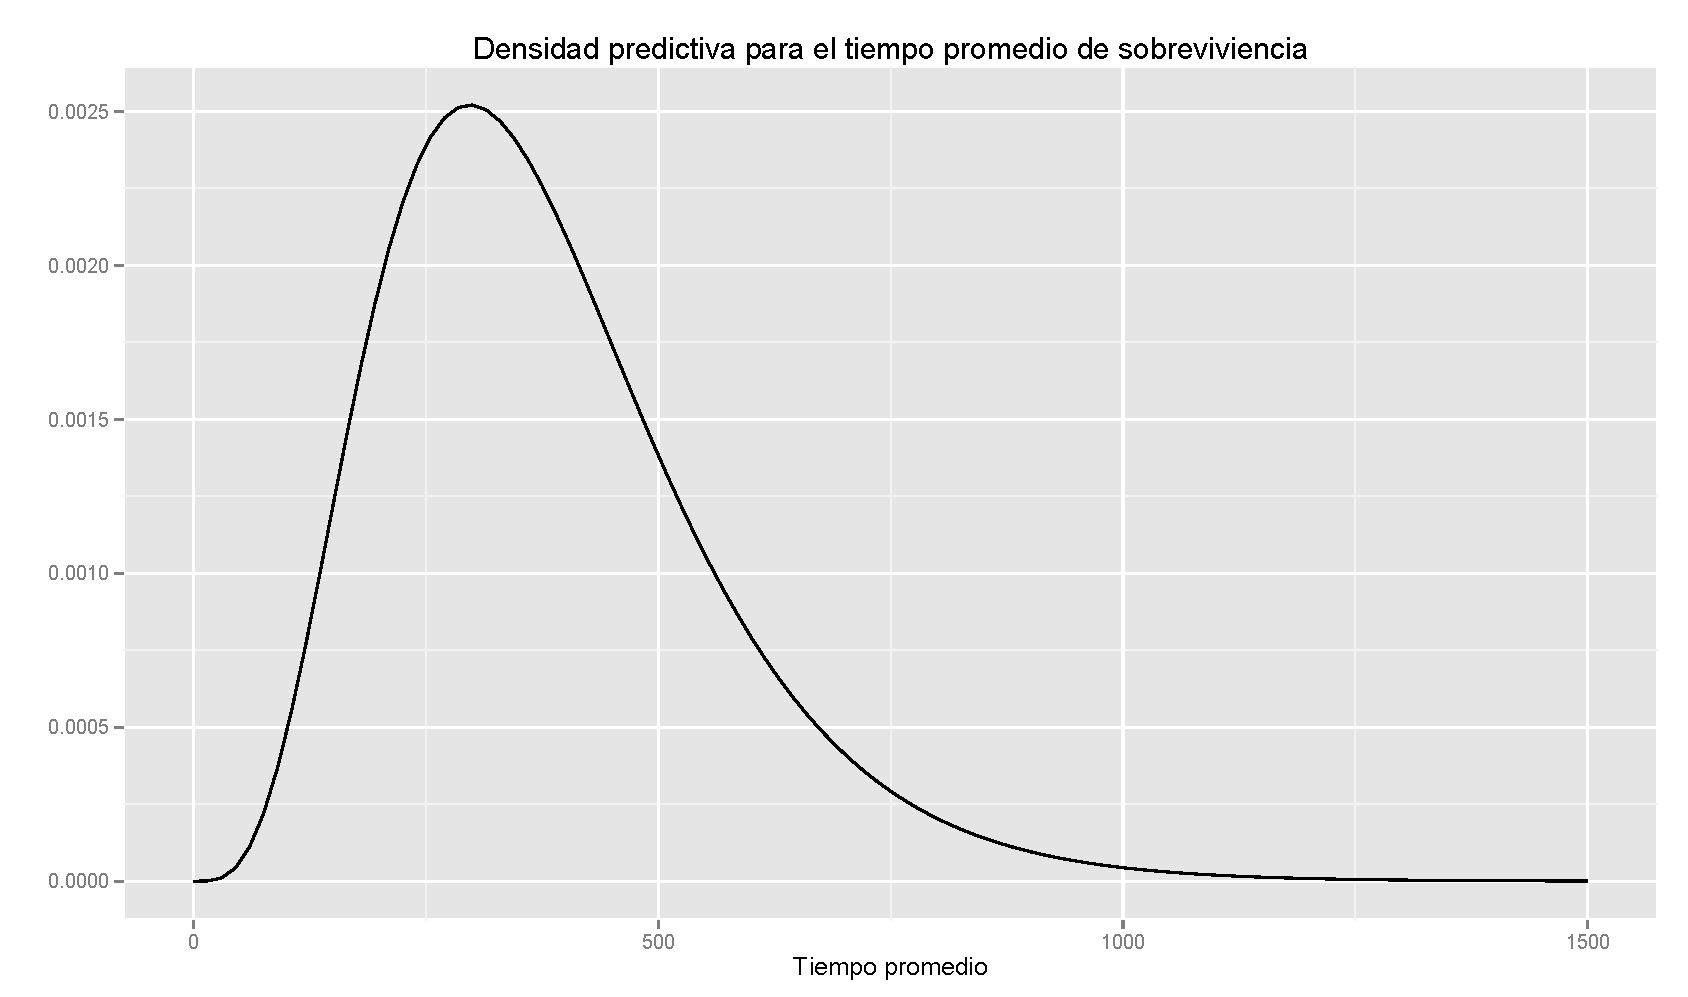
\includegraphics[scale=0.4]{predexponencial.pdf}
    \caption{\emph{Distribuci\'on predictiva posterior para el tiempo promedio de sobrevivencia de transplante de coraz\'on.}}
    \label{pred_post_expo_eje}
    \end{figure}
    
    \section{Modelo normal con media desconocida y varianza conocida}
    
    En esta \'ultima secci\'on de este cap\'itulo, se considera datos que pueden ser descritos adecuadamente con la distribuci\'on normal, la cual a diferencia de las anteriores distribuciones consideradas tiene dos par\'ametros. En el siguiente cap\'itulo se considera el caso general cuando ambos par\'ametros son desconocidos. En esta parte, se asume que la varianza te\'orica es conocica, y el objetivo es estimar la media te\'orica.
    
    Suponga que $Y_1,\cdots,Y_n$ son variables independientes e id\'enticamente distribuidos con distribuci\'on $Normal(\theta,\sigma^2)$ con $\theta$ desconcido pero $\sigma^2$ conocido. De esta forma, la funci\'on de verosimilitud de los datos est\'a dada por
    \begin{align}
    \label{vero_normal}
    p(\mathbf{Y} \mid \theta)&=\prod_{i=1}^n\frac{1}{\sqrt{2\pi\sigma^2}}\exp\left\{-\frac{1}{2\sigma^2}(y_i-\theta)^2\right\}I_\mathbb{R}(y)\notag\\
    &=(2\pi\sigma^2)^{-n/2}\exp\left\{-\frac{1}{2\sigma^2}\sum_{i=1}^n(y_i-\theta)^2\right\}
    \end{align}
    
    Como el par\'ametro $\theta$ puede tomar cualquier valor en los reales, es posible asignarle una distribuci\'on previa $\theta \sim Normal(\mu,\tau^2)$. Bajo este marco de referencia se tienen los siguientes resultados
    
    \begin{Res}\label{Res_pos_theta}
    La distribuci\'on posterior del par\'ametro de inter\'es $\theta$ sigue una distribuci\'on
    \begin{equation*}
    \theta|\mathbf{Y} \sim Normal(\mu_n,\tau^2_n).
    \end{equation*}
    En donde
    \begin{equation}\label{tau_sigma_n}
    \mu_n=\frac{\frac{n}{\sigma^2}\bar{Y}+\frac{1}{\tau^2}\mu}{\frac{n}{\sigma^2}+\frac{1}{\tau^2}}
    \ \ \ \ \ \ \ \text{y} \ \ \ \ \ \ \
    \tau_n^2=\left(\frac{n}{\sigma^2}+\frac{1}{\tau^2}\right)^{-1}
    \end{equation}
    \end{Res}
    
    \begin{proof}
    \begin{align*}
    p(\theta \mid \mathbf{Y})&\propto p(\mathbf{Y} \mid \theta)p(\theta \mid \mu,\tau^2)\\
    &\propto \exp\left\{-\frac{1}{2\sigma^2}\sum_{i=1}^n(y_i-\theta)^2-\frac{1}{2\tau^2}(\theta-\mu)^2\right\}\\
    &= \exp\left\{-\frac{1}{2}\left[\frac{\sum_{i=1}^n(y_i-\theta)^2}{\sigma^2}+\frac{(\theta-\mu)^2}{\tau^2}\right]\right\}\\
    &\propto \exp\left\{-\frac{1}{2}\left[\frac{n\theta^2}{\sigma^2}-\frac{2\theta\sum_{i=1}^ny_i}{\sigma^2}+\frac{\theta^2}{\tau^2}-\frac{2\theta\mu}{\tau^2}\right]\right\}\\
    &= \exp\left\{-\frac{\theta^2}{2}\left[\frac{n}{\sigma^2}+\frac{1}{\tau^2}\right]+
    \theta\left[\frac{n\bar{y}}{\sigma^2}+\frac{\mu}{\tau^2}\right]\right\}\\
    &= \exp\left\{-\frac{\theta^2}{2\tau^2_n}+\frac{\theta\mu_n}{\tau_n^2}\right\}\\
    &= \exp\left\{-\frac{1}{2\tau^2_n}(\theta^2-2\theta\mu_n)\right\}\\
    &\propto \exp\left\{-\frac{1}{2\tau^2_n}(\theta^2-2\theta\mu_n+\mu_n^2)\right\}\\
    &= \exp\left\{-\frac{1}{2\tau^2_n}(\theta-\mu_n)^2\right\}
    \end{align*}
    Por lo tanto, se encuentra una expresi\'on id\'entica a la funci\'on de distribuci\'on de una variable aleatoria con distribuci\'on $Normal(\mu_n,\tau_n^2)$.
    \end{proof}
    
    Observando la forma de $\mu_n$, que corresponde a la estimaci\'on bayesiana del par\'ametro $\theta$, podemos concluir que \'este es una combinaci\'on convexa entre el estimador cl\'asico de m\'axima verosimlitud $\hat{\theta}_C=\bar{y}$ y el estimador previo $\hat{\theta}_P=\mu$, puesto que:
    \begin{align*}
    \hat{\theta}_B=\mu_n&=\frac{\frac{n}{\sigma^2}\bar{Y}+\frac{1}{\tau^2}\mu}{\frac{n}{\sigma^2}+\frac{1}{\tau^2}}\\
    &=\frac{\frac{n}{\sigma^2}}{\frac{n}{\sigma^2}+\frac{1}{\tau^2}}\bar{Y}+\frac{\frac{1}{\tau^2}}{\frac{n}{\sigma^2}+\frac{1}{\tau^2}}\mu\\
    &=\frac{\frac{n}{\sigma^2}}{\frac{n}{\sigma^2}+\frac{1}{\tau^2}}\hat{\theta}_C+\frac{\frac{1}{\tau^2}}{\frac{n}{\sigma^2}+\frac{1}{\tau^2}}\hat{\theta}_P\\
    \end{align*}
    
    De donde se puede concluir que para una distribuci\'on previa fija, entre mayor sea el tama\~no muestral $n$, m\'as peso tendr\'a el estimador cl\'asico $\hat{\theta}_C$ en el c\'alculo del estimador bayesiano. De la misma forma, para un conjunto fijo de datos $\mathbf{Y}$, entre menor sea la varianza previa, $\tau^2$, m\'as certeza tenemos sobre la informaci\'on previa y por consiguiente la estimaci\'on bayesiana $\mu_n$ se acercar\'a m\'as a la estimaci\'on previa. En la Figura \ref{compara_normal} se observa la funci\'on de densidad previa, funci\'on de verosimilitud y funci\'on de densidad posterior con $\mu=5$, $\tau^2=0.01$, $\bar{y}=2$, $\sigma^2=1$ y $n=5,10,50,200$. Podemos observar que a medida que el tama\~no muestral $n$ aumente, la funci\'on de verosimilitud (vista como la funci\'on del par\'ametro $\theta$) se vuelve m\'as concentrada alrededor del valor de $\bar{y}$, y a consecuencia, la funci\'on de densidad posterior de $\theta$ se sit\'ua m\'as cercana a la funci\'on de verosimilitud, y la estimaci\'on bayesiana se acerca m\'as a la estimaci\'on cl\'asica $\bar{y}$.
    
    \begin{figure}[!h]
    \centering
    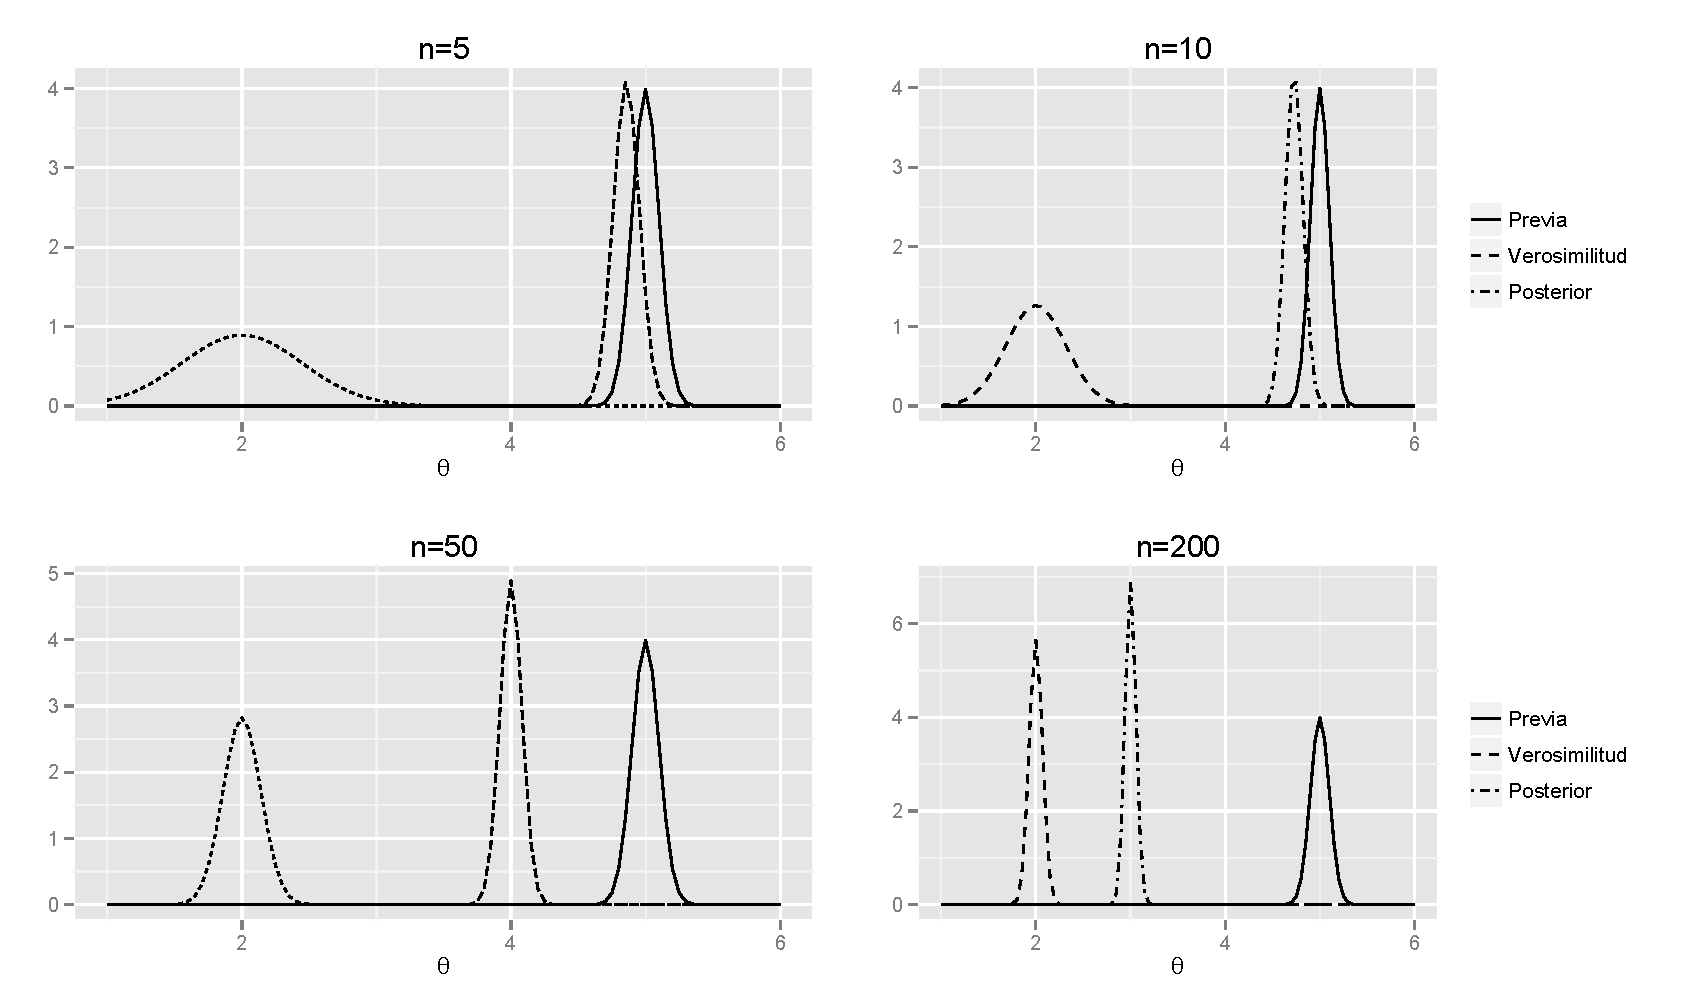
\includegraphics[scale=0.57]{Comparacion_Normal.pdf}
    \caption{\emph{Distribuci\'on previa, funci\'on de verosimilitud y distribuci\'on posterior del par\'ametro $\theta$ con $\mu=5$, $\tau^2=0.01$, $\bar{y}=2$, $\sigma^2=1$ y $n=5,10,50,200$.}}
    \label{compara_normal}
    \end{figure}
    
    \textbf{\emph{Distribuci\'on previa no informativa para $\theta$}}
    
    Por otro lado, n\'otese que en el caso en donde se desconozca el comportamiento estructural de $\theta$, es posible hacer su distribuci\'on previa tan plana y vaga como sea posible. Para esto, basta con hacer tender al par\'ametro de precisi\'on de la distribuci\'on previa hacia infinito. Es decir $\tau^2 \longrightarrow \infty$, en este caso, la distribuci\'on previa de $\theta$ corresponde a una distribuci\'on impropia, $p(\theta)\propto cte$. Se puede ver que bajo esta distribuci\'on previa, la distribuci\'on posterior tender\'ia a una $Normal(\bar{y},\sigma^2/n)$ (Ejercicio XXXX).
    
    La anterior idea intuitiva de usar la distribuci\'on previa $p(\theta)\propto cte$ para representar la falta de la informaci\'on previa corresponde a la previa no informativa de Jeffreys, puesto que la informaci\'on de Fisher del par\'ametro $\theta$ en una variable con distribuci\'on normal est\'a dada por 
    \begin{equation*}
    I(\theta)=1/\sigma^2
    \end{equation*}
    
    De donde se puede concluir qua la previa no informativa de Jeffreys est\'a dada por 
    \begin{equation*}
    p(\theta)\propto 1/\sigma\propto cte
    \end{equation*}
    
    Se puede ver que cuando se utiliza la anterior distribuci\'on previa para $\theta$, la distribuci\'on posterior est\'a dada por (Ejercicio \ref{XXX})
    \begin{equation*}
    \theta\mid\mathbf{Y}\sim Normal\left(\bar{y},\ \dfrac{\sigma^2}{n}\right)
    \end{equation*}
    
    Finalmente, comparemos los resultados inferenciales obtenidos con la previa no informativa de Jeffreys con el enfoque inferencial cl\'asico en t\'erminos de la estimaci\'on puntua y el intervalo de credibilidad y de confianza.
    
    \begin{itemize}
    \item En cuanto a la estimaci\'on puntual, es claro que ambos enfoques conducen al mismo estimador $\hat{\theta}=\bar{Y}$.
    \item Con respecto al intervalo para el par\'ametro $\theta$, al usar el enforque bayesiano con la previa no informativa de   Jeffreys, un intervalo de credibilidad de $(1-\alpha)\times 100\%$ est\'an dadas por los percentiles $\alpha/2$ y $1-\alpha   /2$ de la distribuci\'on posterior de $\theta$: $Normal(\bar{y},\sigma^2/n)$, denotaremos estos percentiles como $a$ y $b$, respectivamente. 
    Por definici\'on tenemos que, si $X\sim N(\bar{y},\sigma^2/n)$,
    \begin{align*}
    \alpha/2&=Pr(X<a)\\
    &=Pr(\frac{X-\bar{y}}{\sigma/\sqrt{n}}<\frac{a-\bar{y}}{\sigma/\sqrt{n}})\\
    &=Pr(Z < \frac{a-\bar{y}}{\sigma/\sqrt{n}})
    \end{align*}
    Estos es, $\frac{a-\bar{y}}{\sigma/\sqrt{n}}$ es el percentil $\alpha/2$ de la distribuci\'on normal est\'andar $z_{\alpha/2}$ \'o equivalentemente $-z_{1-\alpha/2}$. De esta forma, tenemos que $a=\bar{y}-z_{1-\alpha/2}\sigma/\sqrt{n}$. An\'alogamente tenemos que $b=bar{y}+z_{1-\alpha/2}\sigma/\sqrt{n}$, y podemos concluir que un intervalo de crediblidad de $(1-\alpha)\times 100\%$ est\'a dada por $\bar{y}\pm z_{1-\alpha/2}\sigma/\sqrt{n}$, el cual coincide con el intervalo de confianza para $\theta$ usando el enfoque de la inferencia cl\'asica \cite{Zhang}.
    \end{itemize}
    
    
    \textbf{\emph{Diferentes formas de hallar la distribuci\'on previa para $\theta$}}
    
    En primer lugar, consideramos el caso cuando la informaci\'on previa se encuentra en un conjunto de datos $x_1,\cdots,x_{m}$ que corresponden a mediciones de la variable de estudio $Y$ en otro punto de tiempo, en otro punto geogr\'afico, o inclusive en otra poblaci\'on de estudio. En este caso, podemos tomar la media de la distribuci\'on previa $\mu$ como $\bar{X}$ y la varianza de la distribuci\'on previa $\tau^2$ como $S^2_X$.
    
    En el caso de que no se dispongan de datos como informaci\'on previa, sino que \'esta est\'a contenida en alguna estimaci\'on que se haya realizado sobre $\theta$. Por ejemplo, si se dispone de alg\'un modelamiento estad\'istico que se haya hecho previamente sobre $\theta$, podemos f\'acilmente obtener el valor estimado de $\theta$ y el error est\'andar de esta estimaci\'on, y naturalmente, estos dos valores ser\'ian nuestros par\'ametros de la distribuci\'on previa: $\mu$ y $\tau^2$. 
    
    Finalmente, si la estimaci\'on previa de $\theta$ se presentada en forma de un intervalo, por ejemplo, si se sabe que un intervalo de confianza para $\theta$ es $(15.3,\ 24.7)$, entonces podemos usar $\mu$ como el punto medio de este intervalo, es decir, $\mu=20$ y para escoger el valor de $\tau^2$, se tiene en cuenta que en muchas ramas de la estad\'istica, un intervalo de confianza se puede aproximar por $\hat{\theta}\pm 2\sqrt{var(\hat{\theta})}$. De esta forma, podemos usar $\tau^2=\left(\frac{24.7-20}{2}\right)^2\approx5.5$
    
    \textbf{\emph{Distribuciones predictivas}}
    
    Ahora, se discute las distribuciones predictivas previa y predictiva posterior para una observaci\'on o una nueva muestra.
    
    \begin{Res}
    La distribuci\'on predictiva previa para una observaci\'on $y$ es
    \begin{equation*}
    y \sim Normal (\mu, \tau^2+\sigma^2)
    \end{equation*}
    \end{Res}
    
    \begin{proof}
    De la definici\'on de funci\'on de distribuci\'on predictiva se tiene que
    \begin{align*}
    p(Y)&=\int p(Y \mid \theta)p(\theta \mid \mu,\tau^2)\ d\theta\\
    &=\int_{-\infty}^{\infty} \frac{1}{\sqrt{2\pi\sigma^2}}\exp\left\{-\frac{1}{2\sigma^2}(y-\theta)^2\right\}
    \frac{1}{\sqrt{2\pi\tau^2}}\exp\left\{-\frac{1}{2\tau^2}(\theta-\mu)^2\right\}d\theta\\
    \end{align*}
    
    \citeasnoun{Berger} desarroll\'o las siguientes igualdades
    \begin{align*}
    &\ \ \ \ \frac{1}{2}\left[\frac{(\theta-\mu)^2}{\tau^2}+\frac{(y-\theta)^2}{\sigma^2}\right]\\
    &=\frac{1}{2}\left[\left(\frac{1}{\tau^2}+\frac{1}{\sigma^2}\right)\theta^2-2\left(\frac{\mu}{\tau^2}+\frac{y}{\sigma^2}\right)\theta+\left(\frac{\mu^2}{\tau^2}+\frac{y^2}{\sigma^2}\right)\right]\\
    &=\frac{1}{2\tau_1^2}\left[\theta^2-2\tau_1^2\left(\frac{\mu}{\tau^2}+\frac{y}{\sigma^2}\right)\theta+\tau_1^4\left(\frac{\mu}{\tau^2}+\frac{y}{\sigma^2}\right)^2\right]+\frac{1}{2}\left(\frac{\mu^2}{\tau^2}+\frac{y^2}{\sigma^2}\right)-\frac{\tau_1^2}{2}\left(\frac{\mu}{\tau^2}+\frac{y}{\sigma^2}\right)^2\\
    &=\frac{1}{2\tau_1^2}\left[\theta-\tau_1^2\left(\frac{\mu}{\tau^2}+\frac{y}{\sigma^2}\right)\right]^2+\frac{1}{2}\left[\left(\frac{1}{\sigma^2}-\frac{\tau_1^2}{\sigma^4}\right)y^2-2\frac{\mu\tau_1^2}{\tau^2\sigma^2}y+\left(\frac{\mu^2}{\tau^2}-\frac{\mu^2\tau_1^2}{\tau^4}\right)\right]\\
    &=\frac{1}{2\tau_1^2}\left[\theta-\mu_1\right]^2+\frac{1}{2}\left[\frac{1}{\sigma^2+\tau^2}y^2-2\frac{\mu}{\sigma^2+\tau^2}y+\frac{\mu^2}{\sigma^2+\tau^2}\right]\\
    &=\frac{1}{2\tau_1^2}\left[\theta-\mu_1\right]^2+\frac{1}{2(\sigma^2+\tau^2)}(y-\mu)^2.
    \end{align*}
    
    
    Entonces
    \begin{align*}
    p(Y)&=\int_{-\infty}^{\infty} \frac{1}{2\pi\sigma\tau}\exp\left\{-\frac{1}{2\tau_1^2}(\theta-\mu_1)^2\right\}
    \exp\left\{-\frac{1}{2(\tau^2+\sigma^2)}(y-\mu)^2\right\}d\theta\\
    &= \frac{1}{\sqrt{2\pi\frac{\sigma^2\tau^2}{\tau_1^2}}}\exp\left\{-\frac{1}{2(\tau^2+\sigma^2)}(y-\mu)^2\right\}
    \int_{-\infty}^{\infty} \frac{1}{\sqrt{2\pi\tau_1^2}}\exp\left\{-\frac{1}{2\tau_1^2}(\theta-\mu_1)^2\right\}d\theta\\
    &= \frac{1}{\sqrt{2\pi(\tau^2+\sigma^2)}}\exp\left\{-\frac{1}{2(\tau^2+\sigma^2)}(y-\mu)^2\right\}
    \end{align*}
    \end{proof}
    
    Una vez recolectados los datos $\mathbf{Y}=\{Y_1,\cdots,Y_n\}$, se obtiene la distribuci\'on predictiva posterior dada en el siguiente resultado. La demostraci\'on es similar al del resultado anterior, y se deja como ejercicio para los lectores.
    \begin{Res}\label{pred_y_theta}
    La distribuci\'on predictiva posterior para una nueva observaci\'on $\tilde{y}$ es
    \begin{equation*}
    \tilde{y} \mid \mathbf{Y} \sim Normal (\mu_n, \tau_n^2+\sigma^2)
    \end{equation*}
    
    cuando se tiene una distribuci\'on previa informativa para $\theta$. 
    
    Cuando se utiliza la distribuci\'on previa no informativa de Jeffreys, la distribuci\'on predictiva posterior para una nueva observaci\'on $\tilde{y}$ es
    \begin{equation*}
    \tilde{y} \mid \mathbf{Y} \sim Normal \left(\bar{y}, \left(1+\dfrac{1}{n}\right)\sigma^2\right)
    \end{equation*}
    \end{Res}
    
    \begin{proof}
    \label{Res_pred_normal}
    Se deja como ejercicio para los lectores.
    \end{proof}
    
    En algunas situaciones, se quiere conocer el comportamiento probabil\'istico de m\'as de una nueva observaci\'on, digamos $Y_1^*,\cdots,Y_{n^*}^*$, en este caso, lo ideal ser\'ia obtener la distribuci\'on conjunta predictiva posterior de la nueva muestra, $p(Y_1^*,\cdots,Y_{n^*}^*|\mathbf{Y})$. Sin embargo, esta distribuci\'on no es f\'acil de hallar, y procedemos a hallar la distribuci\'on predictiva posterior de la media de esta nueva muestra $\bar{Y}^*$, la cual es dada en el siguiente resultado. 
    
    \begin{Res}\label{pred_norm}
    La distribuci\'on predictiva posterior para la media muestral $\bar{Y}^*$ de una nueva muestra es 
    \begin{equation*}
    \bar{Y}^*|\mathbf{Y}\ \sim N\left(\mu_n, \frac{\sigma^2}{n^*}+\tau^2_n\right)
    \end{equation*}
    cuando se tiene una previa informativa para $\theta$, $\mu_n$ y $\tau^2_n$ fueron definidos en (\ref{tau_sigma_n}).
    
    Cuando se utiliza la distribuci\'on previa no informativa de Jeffreys para $\theta$, la distribuci\'on predictiva posterior para la media muestral $\bar{Y}^*$ de una nueva muestra es 
    \begin{equation*}
    \bar{Y}^*|\mathbf{Y}\ \sim N\left(\bar{y}, \left(\dfrac{1}{n}+\dfrac{1}{n^*}\right)\sigma^2\right).
    \end{equation*}
    \end{Res}
    
    \begin{proof}
    Primero, consideramos cuando la distribuci\'on previa de $\theta$ es $N(\mu,\tau^2)$, tenemos que:
    \begin{align*}
    p(\bar{Y}^*|\mathbf{Y})&=\int_{-\infty}^\infty p(\bar{Y}^*|\theta)p(\theta|\mathbf{Y})\ d\theta\\
    &=\int_{-\infty}^\infty (2\pi\frac{\sigma^2}{n^*})^{-1/2}\exp\left\{-\frac{n^*}{2\sigma^2}(\bar{y}^*-\theta)^2\right\}
    (2\pi\tau_n^2)^{-1/2}\exp\left\{-\frac{1}{2\tau_n^2}(\theta-\mu_n)^2\right\}\ d\theta\\
    &=\int_{-\infty}^\infty (2\pi)^{-1}(\frac{\sigma^2}{n^*}\tau_n^2)^{-1/2}\exp\left\{-\frac{1}{2}\left[\frac{(\bar{y}^*-\theta)^2}{\sigma^2/n^*}+\frac{(\theta-\mu_n)^2}{\tau^2_n}\right]\right\}\ d\theta\\
    &=\underbrace{\int_{-\infty}^\infty(2\pi\frac{1}{n^*/\sigma^2+1/\tau^2_n})^{-1/2}\exp\left\{-\frac{1}{2}\left(\frac{n^*}{\sigma^2}+\frac{1}{\tau^2_n}\right)\left(\theta-\frac{\bar{y}^*/(\sigma^2/n^*)+\mu_n/\tau^2_n}{n^*/\sigma^2+1/\tau^2_n}\right)^2\right\}\ d\theta}_{\text{igual a 1}}\\
    &\ \ \ \ \ \ \ (2\pi)^{-1/2}(\frac{\sigma^2}{n^*}\tau_n^2)^{-1/2}(\frac{n^*}{\sigma^2}+\frac{1}{\tau^2_n})^{-1/2}\exp\left\{-\frac{1}{2(\sigma^2/n^*+\tau^2_n)}(\bar{y}^*-\mu_n)^2\right\}\\
    &=(2\pi)^{-1/2}(\frac{\sigma^2}{n^*}\tau_n^2)^{-1/2}(\frac{n^*}{\sigma^2}+\frac{1}{\tau^2_n})^{-1/2}\exp\left\{-\frac{1}{2(\sigma^2/n^*+\tau^2_n)}(\bar{y}^*-\mu_n)^2\right\}\\
    &=(2\pi)^{-1/2}(\frac{\sigma^2}{n^*}+\tau^2_n)^{-1/2}\exp\left\{-\frac{1}{2(\sigma^2/n^*+\tau^2_n)}(\bar{y}^*-\mu_n)^2\right\}
    \end{align*}
    
    Los desarrollos para cuando se utiliza la distribuci\'on previa no informativa de Jeffreys es similar, y se deja para los lectores (Ejercicio \ref{Ejer_pre_Jeffreys}). 
    \end{proof}
    
    Del anterior resultado, podemos ver que (1) la esperanza de la distribuci\'on de $\bar{Y}^*|\mathbf{Y}$ es igual a la esperanza de $\theta|\mathbf{Y}$, y (2) a diferencia de la varianza de $\theta|\mathbf{Y}$, la varianza de $\bar{Y}^*|\mathbf{Y}$ tiene un componente adicional: $\sigma^2/n^*$, de esta forma, tenemos tres fuentes de incertidumbre al momento de pronosticar $\bar{Y}^*$: la incertidumbre en la informaci\'on previa, la incertidumbre en la muestra observada y la incertidumbre en la nueva muestra.
    
    \begin{Eje}\label{eje_vidrios}
    En \citeasnoun[Ejemplo 2.3.6]{Zhang} reportan datos sobre el grosor de l\'aminas de vidrio templado de 3cm para controlar la calidad de los vidrios producidos por una l\'inea de producci\'on con el fin de conocer el grosor real de las l\'aminas producidas. Estos datos son: 3.56, 3.36, 2.99, 2.71, 3.31, 3.68, 2.78, 2.95, 2.82, 3.45, 3.42 y 3.15, con el promedio de 3.18cm. Suponga que por especificaciones t\'ecnicas, se conoce que la varianza del grosor es de $0.1\text{cm}^2$. Por otro lado como informaci\'on previa, se conoce que en la \'ultima inspecci\'on de calidad, se conoce que el grosor promedio fue de 2.8cm con una desviaci\'on est\'andar de 0.23cm.
    
    De la anterior informaci\'on, se puede decir que el par\'ametro de inter\'es $\theta$ ser\'ia el grosor promedio de las l\'aminas. Tambi\'en podemos afirmar que $\sigma^2=0.1cm^2$, $\bar{y}=3.18cm$, $n=12$, y los par\'ametros de la distribuci\'on previa est\'an dados por $\mu=2.8cm$ y $\tau=0.45cm$, de esta forma, podemos calcular los par\'ametros de la distribuci\'on posterior
    \begin{align*}
    \mu_n&=\dfrac{\frac{12}{0.1}3.18+\frac{1}{0.23^2}2.8}{\frac{12}{0.1}+\frac{1}{0.23^2}}=3.13cm\\
    \tau^2_n&=\left(\frac{12}{0.1}+\frac{1}{0.23^2}\right)^{-1}=0.007cm^2\\
    \end{align*}
    
    Entonces la distribuci\'on posterior del grosor promedio es $N(\mu_n=3.13cm,\ \tau^2_n=0.007cm^2)$. Podemos concluir que la estimaci\'on bayesiana del par\'ametro corresponde a $3.13cm$, mientras que para calcular un intervalo de credibilidad de $95\%$ para el par\'ametro de inter\'es, se debe calcular los percentiles $2.5\%$ y $97.5\%$ de la distribuci\'on posterior de $\theta$, y el intervalo de credibilidad queda dado por $(2.966cm,\ 3.293cm)$.
    
    A continuaci\'on se ilustra el uso de \verb'JAGS' para obtener la estimaci\'on bayesiana del par\'ametro $\theta$.
    
    \colorbox{black}{\textcolor{white}{\textbf{C\'odigo JAGS}}}
\begin{knitrout}
\definecolor{shadecolor}{rgb}{0.933, 0.933, 0.933}\color{fgcolor}\begin{kframe}
\begin{alltt}
\hlstd{Norm.model} \hlkwb{<-} \hlkwa{function}\hlstd{()\{}
\hlkwa{for}\hlstd{(i} \hlkwa{in} \hlnum{1} \hlopt{:} \hlstd{n)}
\hlstd{\{}
\hlstd{y[i]} \hlopt{~} \hlkwd{dnorm}\hlstd{(theta,} \hlnum{1}\hlopt{/}\hlnum{0.1}\hlstd{)}
\hlstd{\}}
\hlstd{theta} \hlopt{~} \hlkwd{dnorm}\hlstd{(}\hlnum{2.8}\hlstd{,} \hlnum{1}\hlopt{/}\hlstd{(}\hlnum{0.23}\hlopt{^}\hlnum{2}\hlstd{) )}
\hlstd{\}}

\hlstd{n} \hlkwb{<-} \hlnum{12}
\hlstd{y} \hlkwb{<-} \hlkwd{c}\hlstd{(}\hlnum{3.56}\hlstd{,} \hlnum{3.36}\hlstd{,} \hlnum{2.99}\hlstd{,} \hlnum{2.71}\hlstd{,} \hlnum{3.31}\hlstd{,} \hlnum{3.68}\hlstd{,} \hlnum{2.78}\hlstd{,} \hlnum{2.95}\hlstd{,} \hlnum{2.82}\hlstd{,} \hlnum{3.45}\hlstd{,} \hlnum{3.42}\hlstd{,} \hlnum{3.15}\hlstd{)}

\hlstd{Norm.data} \hlkwb{<-} \hlkwd{list}\hlstd{(}\hlstr{"y"}\hlstd{,}\hlstr{"n"}\hlstd{)}
\hlstd{Norm.param} \hlkwb{<-} \hlkwd{c}\hlstd{(}\hlstr{"theta"}\hlstd{)}
\hlstd{Norm.inits} \hlkwb{<-} \hlkwa{function}\hlstd{()\{}
\hlkwd{list}\hlstd{(}\hlstr{"theta"}\hlstd{=}\hlkwd{c}\hlstd{(}\hlnum{3.2}\hlstd{))}
\hlstd{\}}

\hlstd{Norm.fit} \hlkwb{<-} \hlkwd{jags}\hlstd{(}\hlkwc{data}\hlstd{=Norm.data,} \hlkwc{inits}\hlstd{=Norm.inits, Norm.param,} \hlkwc{n.iter}\hlstd{=}\hlnum{10000}\hlstd{,}
\hlkwc{n.burnin}\hlstd{=}\hlnum{1000}\hlstd{,} \hlkwc{model.file}\hlstd{=Norm.model)}
\end{alltt}
\begin{verbatim}
## Compiling model graph
##    Resolving undeclared variables
##    Allocating nodes
## Graph information:
##    Observed stochastic nodes: 12
##    Unobserved stochastic nodes: 1
##    Total graph size: 45
## 
## Initializing model
\end{verbatim}
\begin{alltt}
\hlkwd{print}\hlstd{(Norm.fit)}
\end{alltt}
\begin{verbatim}
## Inference for Bugs model at "/var/folders/n7/01szs8_x7pq1bvpwwnvq7w_w0000gn/T//RtmpMtD1jH/model11b779fb6f8b.txt", fit using jags,
##  3 chains, each with 10000 iterations (first 1000 discarded), n.thin = 9
##  n.sims = 3000 iterations saved
##          mu.vect sd.vect  2.5%   25%   50%   75%  97.5%  Rhat n.eff
## theta      3.132   0.083 2.970 3.076 3.131 3.189  3.298 1.001  3000
## deviance   7.294   1.502 6.171 6.298 6.730 7.669 11.558 1.002  2700
## 
## For each parameter, n.eff is a crude measure of effective sample size,
## and Rhat is the potential scale reduction factor (at convergence, Rhat=1).
## 
## DIC info (using the rule, pD = var(deviance)/2)
## pD = 1.1 and DIC = 8.4
## DIC is an estimate of expected predictive error (lower deviance is better).
\end{verbatim}
\end{kframe}
\end{knitrout}
    De donde podemos ver que la estimaci\'on bayesiana de $\theta$ es 3.132cm, mientras que un intervalo de credibilidad del 95\% es $(2.97cm,\ 3.298cm)$, resultados muy similares a lo obtenido calculando directamente $\mu_n$ y $\tau^2_n$.
    
    Finalmente, ilustramos el uso de la distribuci\'on predictiva posterior. Suponga que la f\'abrica debe hacer un despacho de 8 l\'aminas, y se quiere conocer sobre el grosor promedio del despacho $\bar{y}^*$. Usando el resultado \ref{pred_norm}, tenemos que la disribuci\'on de $\bar{Y}^*$ condicionado en los 12 datos observados est\'a dado por 
    \begin{equation*}
    \bar{Y}^*|\mathbf{Y}\ \sim N\left(\mu_n,\ \frac{\sigma^2}{n^*}+\tau^2_n\right) = N\left(3.13cm,\ \frac{0.1}{8}+0.007\ cm^2\right) = N(3.13cm,\ 0.0195cm^2)
    \end{equation*}
    
    De esta forma, podemos afirmar que el grosor promedio del despacho es de 3.13cm con un intervalo de 95\% dado por los percentiles 2.5\% y 97.5\% de la anterior distribuci\'on: (2.85cm, 3.40cm). N\'otese que el intervalo para $\bar{Y}^{*}$ es m\'as ancho que el intervalo para $\theta$, pues este tiene una varianza mayor a la varianza de la distribuci\'on posterior de $\theta$.
    
    Tambi\'en podemos calcular el intervalo para $\bar{Y}^*$ desde el punto de vista de simulaci\'on, simulando valores de $\theta$ desde su distribuci\'on posterior, y luego simulando valores de $\bar{Y}^*$ desde $p(\bar{Y}^*\mid\theta)$. Los siguientes c\'odigos implemtan este enforque con 5000 iteraciones. Podemos ver que los resultados obtenidos son casi id\'enticos a los calculados anteriormente.
\begin{knitrout}
\definecolor{shadecolor}{rgb}{0.933, 0.933, 0.933}\color{fgcolor}\begin{kframe}
\begin{alltt}
\hlstd{y.bar} \hlkwb{<-} \hlkwd{c}\hlstd{()}
\hlstd{mu.n} \hlkwb{<-} \hlnum{3.13}\hlstd{; tau2.n} \hlkwb{<-} \hlnum{0.007}\hlstd{; sigma2} \hlkwb{<-} \hlnum{0.1}
\hlkwa{for}\hlstd{(i} \hlkwa{in} \hlnum{1}\hlopt{:}\hlnum{5000}\hlstd{)\{}
\hlstd{theta} \hlkwb{<-} \hlkwd{rnorm}\hlstd{(}\hlnum{1}\hlstd{, mu.n,} \hlkwd{sqrt}\hlstd{(tau2.n))}
\hlstd{y.bar[i]} \hlkwb{<-} \hlkwd{rnorm}\hlstd{(}\hlnum{1}\hlstd{, theta,} \hlkwd{sqrt}\hlstd{(sigma2}\hlopt{/}\hlnum{8}\hlstd{))}
\hlstd{\}}
\hlkwd{mean}\hlstd{(y.bar)}
\end{alltt}
\begin{verbatim}
## [1] 3.127
\end{verbatim}
\begin{alltt}
\hlkwd{quantile}\hlstd{(y.bar,} \hlkwd{c}\hlstd{(}\hlnum{0.025}\hlstd{,}\hlnum{0.975}\hlstd{))}
\end{alltt}
\begin{verbatim}
##  2.5% 97.5% 
## 2.854 3.397
\end{verbatim}
\end{kframe}
\end{knitrout}
    \end{Eje}
    
    \section{Modelo normal con varianza desconocida y media conocida}\label{Normal_Varianza}
    
    En esta secci\'on consideramos variables independientes e id\'enticamente distribuidas $Y_1,\cdots,Y_n\sim N(\theta,\sigma^2)$. Asumimos que $\theta$ es conocida y el par\'ametro de inter\'es es $\sigma^2$. En la pr\'actica es inusual encontrar situaciones donde este supuesto se cumpla, sin embargo, los desarrollos presentados en esta secci\'on ser\'an \'utiles en el siguiente cap\'itulo cuando se aborda la distribuci\'on normal con ambos par\'ametros desconocidos. 
    
    Para desarrollar la estimaci\'on bayesiana para $\sigma^2$, el primer paso es asignarle una distribuci\'on previa que sea acorde con los valores que toma el par\'ametro, y en lo posible inducir una distribuci\'on posterior conjugada. De esta forma, observamos que el par\'ametro $\sigma^2$ es estrictamente positivo, y la distribuci\'on previa debe tener soporte \'unicamente los valores positivos. Si bien la distribuci\'on que primero viene a mente ser\'ia la distribuci\'on Gamma, al observar la funci\'on de verosimilitud dada en \ref{vero_normal}, es claro que esta opci\'on no inducir\'a una distribuci\'on posterior conjugado. Por lo tanto recurrimos a la distribuci\'on Inversa-Gamma que tiene la siguiente funci\'on de densidad:
    \begin{equation*}
    f(x)=\dfrac{\beta^\alpha}{\Gamma(\alpha)}x^{-\alpha-1}\exp\left\{-\frac{\beta}{x}\right\}
    \end{equation*}
    
    para $x>0$. $\alpha>0$ es el par\'ametro de forma y $\beta>0$ es el par\'ametro de escala, y usamos la notacion $X\sim Inversa-Gamma(\alpha,\beta)$. Se tiene que para esta distribuci\'on, $E(X)=\frac{\beta}{\alpha-1}$ cuando $\alpha>1$ y $Var(X)=\frac{\beta^2}{(\alpha-1)^2(\alpha-2)}$ cuando $\alpha>2$.
    
    En la literatura se acostumbra usar la siguiente distribuci\'on previa para el par\'ametro $\sigma^2$:
    \begin{equation*}
    \sigma^2 \sim Inversa-Gamma(n_0/2,\ n_0\sigma^2_0/2)
    \end{equation*}
    
    La esperanza previa $\sigma^2$ viene dada por
    \begin{equation*}
    E(\sigma^2)=\dfrac{\frac{n_0\sigma^2_0}{2}}{\frac{n_0}{2}-1}=\dfrac{n_0\sigma^2_0}{n_0-2}\approx\sigma^2_0
    \end{equation*}
    
    y
    \begin{equation*}
    Var(\sigma^2)=\dfrac{\left(\frac{n_0\sigma^2_0}{2}\right)^2}{\left(\frac{n_0}{2}-1\right)\left(\frac{n_0}{2}-2\right)}\approx \dfrac{2\sigma^4_0}{n_0}
    \end{equation*}
    
    De donde podemos escoger el par\'ametro $\sigma^2_0$ como  el valor que se cree apropiado para $\sigma^2$ con base en la informaci\'on previa. $n_0$ denota el n\'umero de datos en la informaci\'on previa, el cual determina el grado de certidumbre del investigador sobre la informaci\'on previa, pues entre mayor sea $n_0$, mayor cantidad de datos representa la distribuci\'on previa, la varianza previa de $\sigma^2$ se hace menor, lo cual representa menor incertidumbre en la distribuci\'on previa.
    
    En la figura \ref{Priori_Sigma2} podemos observar la forma de la distribuci\'on previa para $\sigma^2$ para diferentes valores de $\sigma^2_0$ y $n_0$. Es claro que la distribuci\'on est\'a concentrada alrededor del valor de $\sigma^2_0$; y para un mismo valor de $\sigma^2_0$, entre mayor sea $n_0$ m\'as concentrada est\'a la funci\'on alrededor de $\sigma^2_0$.
    \begin{figure}[!h]
    \centering
    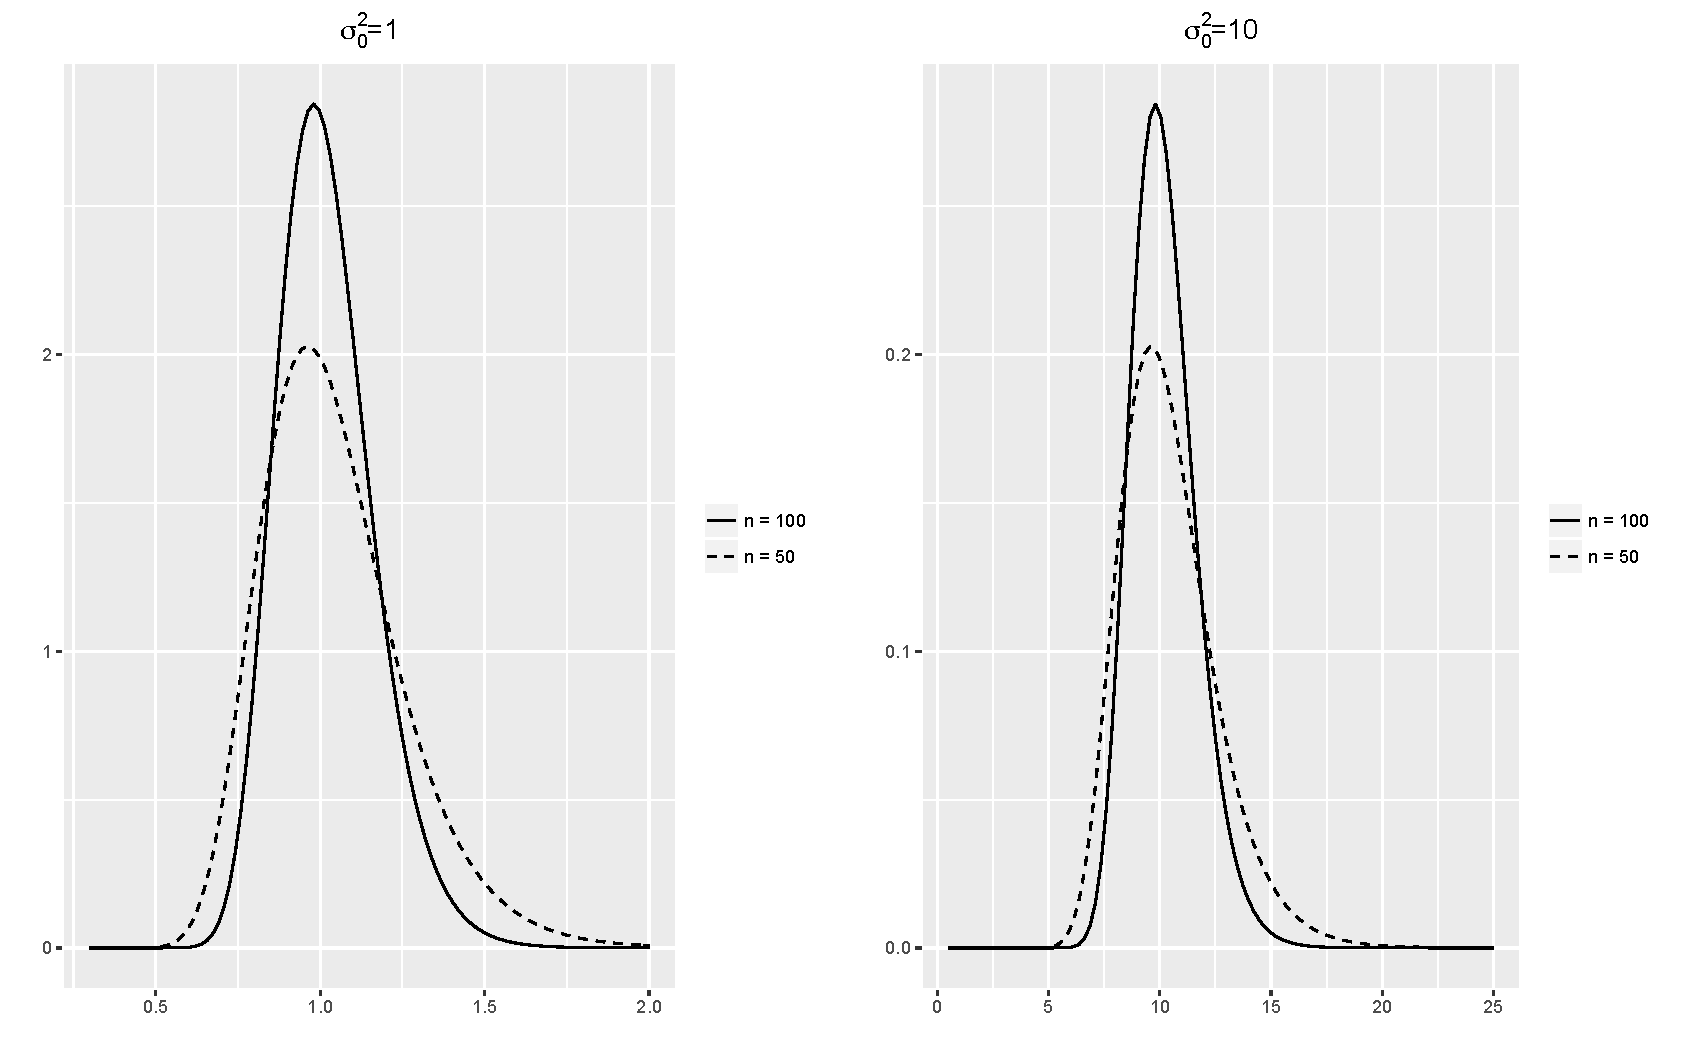
\includegraphics[scale=0.5]{Priori_Sigma2.pdf}
    \caption{\emph{Funci\'on de densidad Inversa-Gamma para diferentes valores de $\sigma^2_0$ y $n_0$.}}
    \label{Priori_Sigma2}
    \end{figure}
    
    Una vez definida la distribuci\'on previa de $\sigma^2$, procedemos a encontrar la distribuci\'on posterior.
    \begin{Res}\label{posterior_sigma2}
    La distribuci\'on posterior de $\sigma^2$ es
    \begin{equation*}
    \sigma^2  \mid \mathbf{Y} \sim Inversa-Gamma\left(\frac{n_0+n}{2},\frac{v_0}{2}\right)
    \end{equation*}
    En donde $v_0=n_0\sigma^2_0+n\hat{\sigma}^2_C$ con $\hat{\sigma}^2_C=\dfrac{1}{n}\sum_{i=1}^n(y_i-\theta)^2$
    \end{Res}
    
    \begin{proof}
    Acudiendo a la distribuci\'on posterior conjunta e incorporando los t\'erminos que no dependen de $\theta$ en la constante de proporcionalidad, se tiene que
    \begin{align*}
    p(\sigma^2 \mid \mathbf{Y})&\propto p(\sigma^2)p(\mathbf{Y}\mid \sigma^2) \\
    &\propto (\sigma^2)^{-n_0/2-1}\exp\left\{-\dfrac{n_0\sigma_0^2}{2\sigma^2}\right\}(\sigma^2)^{-n/2}\exp\left\{-\frac{1}{2\sigma^2}\sum_{i=1}^n(y_i-\theta)^2\right\}\\
    &= (\sigma^2)^{-(n_0+n)/2-1}\exp\left\{-\frac{1}{2\sigma^2}\left[n_0\sigma_0^2+n\hat{\sigma}^2_C\right]\right\}
    \end{align*}
    
    donde $\hat{\sigma}^2_C$ es el estimador cl\'asico de $\sigma^2$ cuando $\theta$ es conocido, definido como $\hat{\sigma}^2_C=\dfrac{1}{n}\sum_{i=1}^n(y_i-\theta)^2$. De esta forma se encuentra la distribuci\'on posterior de $\sigma^2$.
    \end{proof}
    
    De la distribuci\'on posterior de $\sigma^2$ se puede observar que la estimaci\'on bayesiana de $\sigma^2$ est\'a dada por 
    \begin{align*}
    \hat{\sigma}^2_B&=\dfrac{\frac{v_0}{2}}{\frac{n_0+n}{2}}\\
    &=\dfrac{n_0\sigma^2_0+n\hat{\sigma}^2_C}{n_0+n-2}\\
    &\approx \dfrac{n_0\sigma^2_0+n\hat{\sigma}^2_C}{n_0+n}\\
    &=\dfrac{n_0}{n_0+n}\sigma^2_0+\dfrac{n}{n_0+n}\hat{\sigma}^2_C
    \end{align*}
    
    Esto es, la estimaci\'on bayesiana viene siendo un promedio ponderado entre la estimaci\'on previa $\sigma^2_0$ y la estimaci\'on cl\'asica $\hat{\sigma}^2_C$, y las ponderaciones depende directa y \'unicamente del n\'umero de datos de las dos fuentes de informaci\'on: $n_0$ y $n$. En la figura \ref{Posterior_Sigma2} se muestra la funci\'on de densidad de la distribuci\'on previa, distribuci\'on posterior y la funci\'on de verosimilitud vista como una funci\'on de $\sigma^2$ con $n_0=20$, $\sigma^2_0=10$, $\hat{\sigma}^2_C=50$, el tama??o muestral es $n=5,20,50,100$. Podemos ver que a medida que a medida que el tama??o muestral $n$ aumenta, la funci\'on de verosimilitud se concentra m\'as alrededor del valor de $\hat{\sigma}^2_C$, y como consecuencia, la funci\'on de densidad posterior de $\sigma^2$ se acerca m\'as a la funci\'on de verosimilitud, y la estimaci\'on bayesiana tambi\'en se asemeja m\'as a la estimaci\'on cl\'asica $\hat{\sigma}^2_C$.
    
    \begin{figure}[!h]
    \centering
    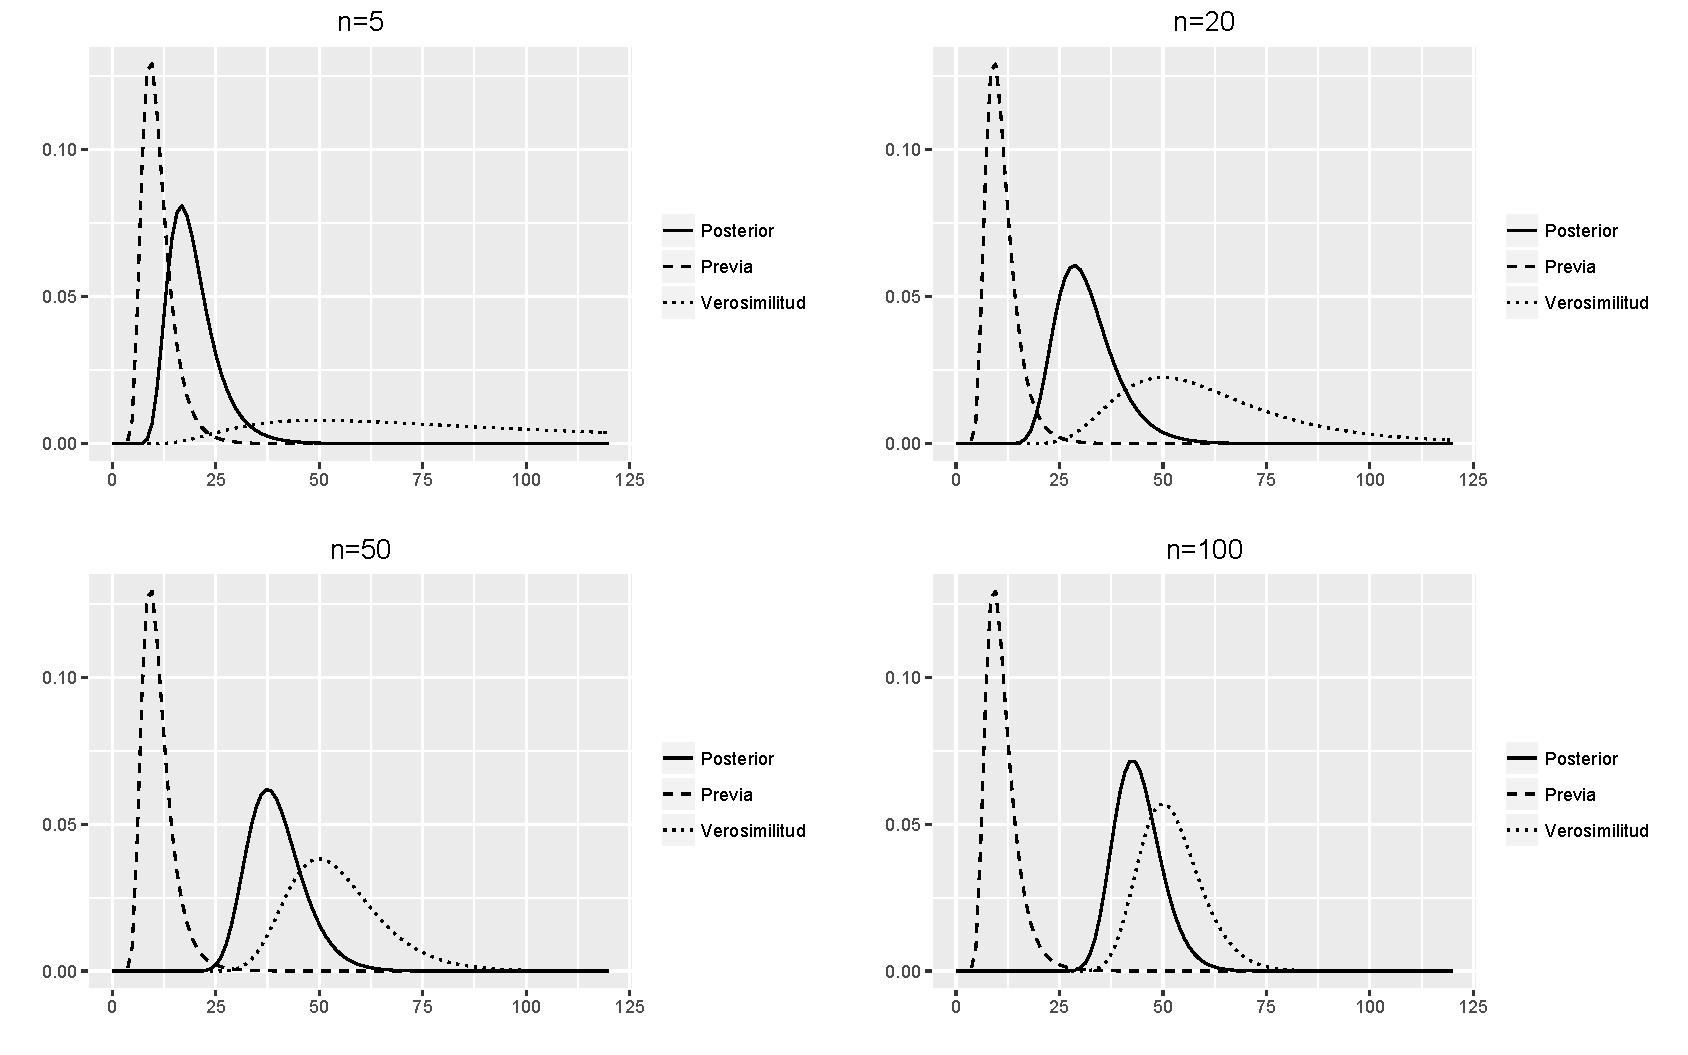
\includegraphics[scale=0.5]{Sigma2_compara.pdf}
    \caption{\emph{Distribuci\'on previa, funci\'on de verosimilitud y distribuci\'on posterior de $\sigma^2$ con $n_0=20$, $\sigma^2_0=10$, $\hat{\sigma}^2_C=50$ y $n=5,20,50,100$.}}
    \label{Posterior_Sigma2}
    \end{figure}
    
    \textbf{\emph{Distribuci\'on previa no informativa para $\sigma^2$}}
    
    Recurriendo a las distribuci\'on previa no informativa de Jeffreys que establece que $p(\theta)\propto I(\theta) ^{1/2}$, donde $\theta$ es el par\'ametro de inter\'es, y $I(\theta)$ es la informaci\'on de Fisher acerca del par\'ametro $\theta$. Despu\'es de algunos c\'alculos se puede ver que (para m\'as detalles, ver \citeasnoun[Sec.2.4]{Zhang})
    \begin{equation*}
    I(\sigma^2)=\dfrac{n}{2\sigma^4}
    \end{equation*}
    
    De esta forma, la distribuci\'on previa no informativa de Jeffreys est\'a dada por $p(\sigma^2)\propto \sigma^{-2}$ para $\sigma^2>0$. Si bien esta distribuci\'on previa es una distribuci\'on impropia (pues $\int_0^\infty p(\sigma^2)=\infty$), al combinar con la funci\'on de verosimilitud, se puede concluir que la distribuci\'on posterior de $\sigma^2$ corresponde a una distribuci\'on Inversa-Gamma con el par\'ametro de forma $n/2$, y par\'ametro de escala $n\hat{\sigma}^2_C/2$ (Ejercicio). En la figura \ref{Posterior_Sigma2_Jeffreys} se puede observar la funci\'on de densidad previa de Jeffreys (\'este ha sido escalado para la \'optima visualizaci\'on), la funci\'on de verosimilitud con $n=50$, $\hat{\sigma}^2_C=10$ y la funci\'on de densidad posterior resultante. Se puede ver claramente que la forma de la distribuci\'on posterior es muy similar a la funci\'on de verosimilitud, de donde se puede intuir que la estimaci\'on bayesiana resulta similar a la estimaci\'on cl\'asica de $\sigma^2$. Efectivamente, podemos ver que cuando se usa la distribuci\'on previa no informativa de Jeffreys, la estimaci\'on bayesiana de $\sigma^2$ corresponde a 
    \begin{align*}
    \hat{\sigma}^2_B&=\dfrac{\frac{n\hat{\sigma}^2_C}{2}}{\frac{n}{2}-1}\\
    &=\dfrac{n}{n-2}\hat{\sigma}^2_C\\
    &\approx \hat{\sigma}^2_C
    \end{align*}
    
    y un intervalo de credibilidad del 95\% queda dado por los percentiles 2.5\% y 97.5\% de la distribuci\'on $Inversa-Gamma(\frac{n}{2},\frac{n\hat{\sigma}^2_C}{2})$.
    
    \begin{figure}[!h]
    \centering
    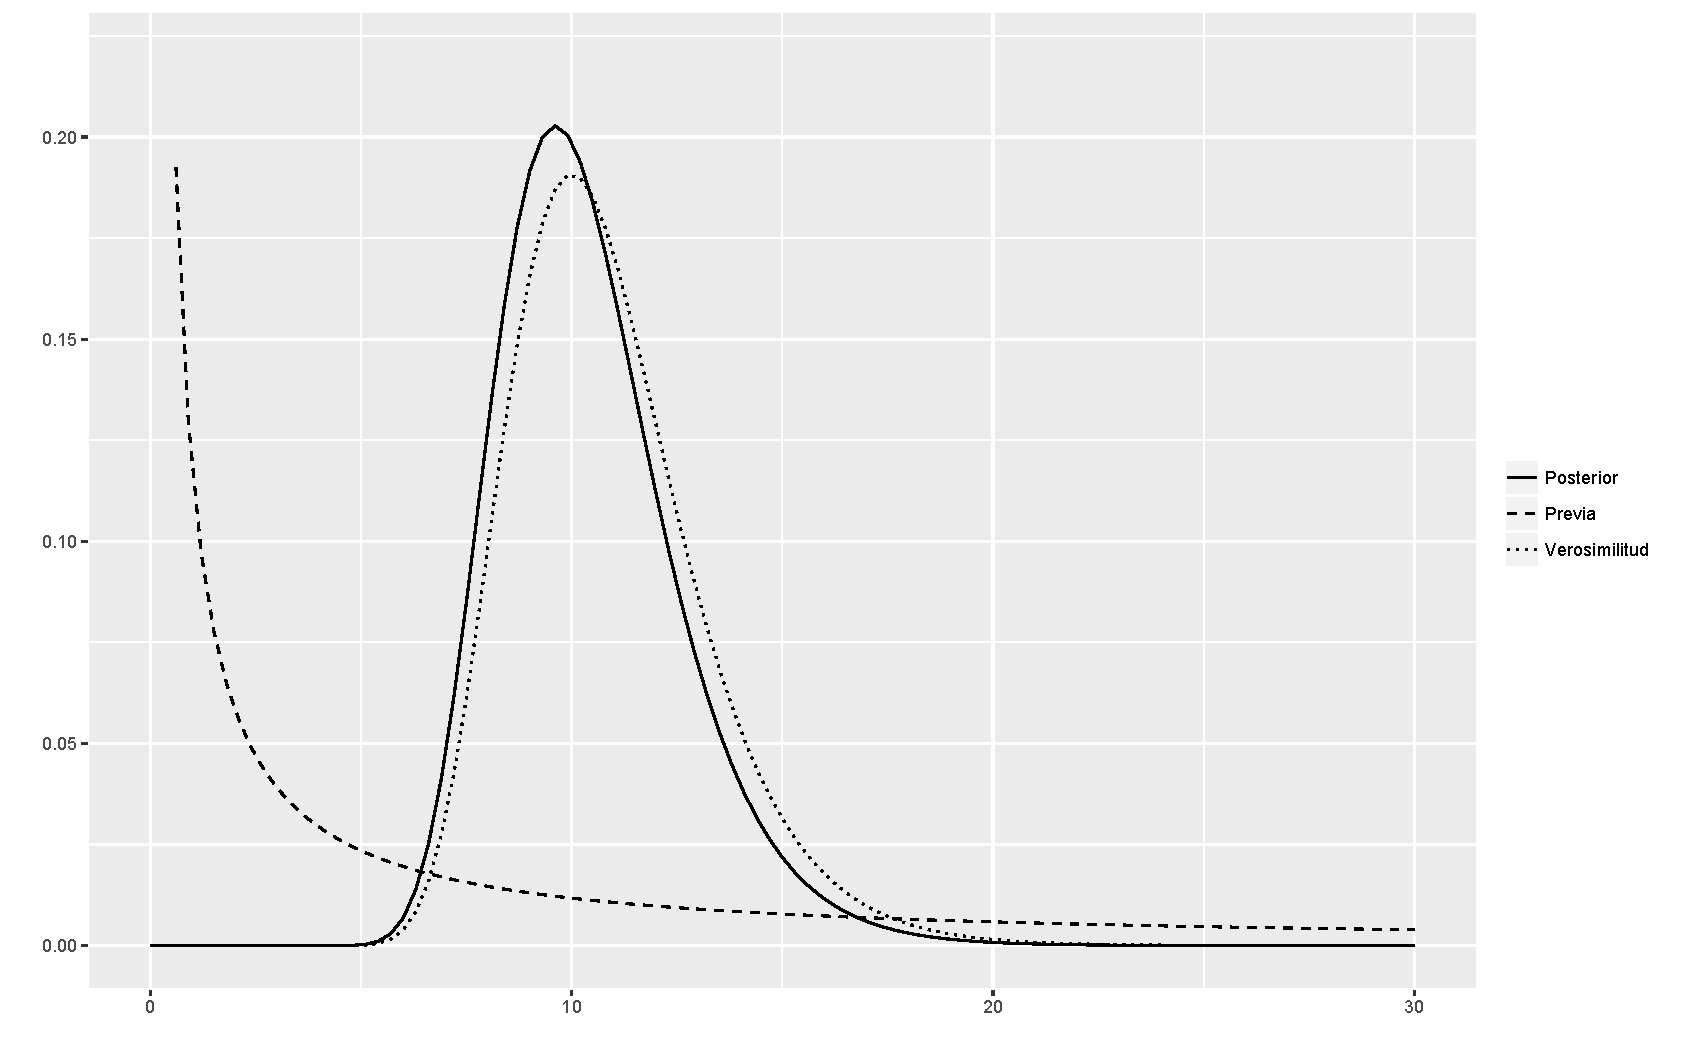
\includegraphics[scale=0.4]{Sigma2_Jeffreys.pdf}
    \caption{\emph{Distribuci\'on previa no informativa de Jeffreys, funci\'on de verosimilitud y distribuci\'on posterior de $\sigma^2$ con $n=50$ y $\hat{\sigma}^2_C=10$.}}
    \label{Posterior_Sigma2_Jeffreys}
    \end{figure}
    
    \textbf{\emph{Distribuci\'on predictiva posterior}}
    
    El siguiente resultado muestra la distribuci\'on predictiva para una nueva observaci\'on $\tilde{y}$.
    \begin{Res}\label{pred_yy_sigma2}
    La distribuci\'on predictiva posterior de una nueva observaci\'on $\tilde{y}$, cuando se utiliza una distribuci\'on previa informativa para $\sigma^2$, es la distribuci\'on $t$ no estandarizado con grado de libertad $n_0+n$, el par\'ametro de localizaci\'on $\theta$ y el par\'ametro de escala $v_0/(n_0+n)$, donde $v_0=n_0\sigma^2_0+\sum_{i=1}^n(y_i-\theta)^2$, esto es, 
    \begin{equation*}
    \tilde{y} \mid \mathbf{Y}\sim t_{n_0+n}\left(\theta,\frac{v_0}{n_0+n}\right).
    \end{equation*} 
    
    Cuando se utiliza la distribuci\'on previa no informativa de Jeffreys para $\sigma^2$, la distrubci\'on predictiva de una nueva observaci\'on $\tilde{y}$ es $t_n(\theta,\hat{\sigma}^2_C)$, con $\hat{\sigma}^2_C=\frac{1}{n}\sum_{i=1}^n(y_i-\theta)^2$. 
    \end{Res}
    
    \begin{proof}
    Cuando la distribuci\'on previa para $\sigma^2$ es $Inversa-Gamma(n_0/2,\ n_0\sigma^2_0/2)$, la distribuci\'on posterior de $\sigma^2$ es $Inversa-Gamma((n_0+n)/2,\ (n_0\sigma^2_0+n\hat{\sigma}^2_C)/2)$, tenemos que 
    \begin{align*}
    p(\tilde{y}\mid\mathbf{Y})&=\int_0^\infty p(\tilde{y}\mid\sigma^2)p(\sigma^2\mid\mathbf{Y})\ d\sigma^2\\
    &=\int_0^\infty (2\pi\sigma^2)^{-1/2}\exp\left\{-\dfrac{1}{2\sigma^2}(\tilde{y}-\theta)^2\right\}\dfrac{(\frac{v_0}{2})^{(n_0+n)/2}(\sigma^2)^{-(n_0+n)/2-1}}{\Gamma(\frac{n_0+n}{2})}\exp\left\{-\dfrac{v_0}{2\sigma^2}\right\}\ d\sigma^2\\
    &=\dfrac{(2\pi)^{-1/2}(\frac{v_0}{2})^{(n_0+n)/2}}{\Gamma(\frac{n_0+n}{2})}\int_0^\infty(\sigma^2)^{-\frac{n_0+n+1}{2}-1}\exp\left\{-\dfrac{1}{\sigma^2}\left[\dfrac{v_0}{2}+\dfrac{1}{2}(\tilde{y}-\theta)^2\right]\right\}\ d\sigma^2\\
    &=\dfrac{(2\pi)^{-1/2}\Gamma(\frac{n_0+n+1}{2})}{\Gamma(\frac{n_0+n}{2})}\left(\frac{v_0}{2}\right)^{(n_0+n)/2}
    \left(\frac{v_0}{2}+\frac{1}{2}(\tilde{y}-\theta)^2\right)^{-\frac{n_0+n+1}{2}}\\
    &=\dfrac{(2\pi)^{-1/2}\Gamma(\frac{n_0+n+1}{2})}{\Gamma(\frac{n_0+n}{2})}\left(\frac{v_0}{2}\right)^{(n_0+n)/2}\left(\frac{v_0}{2}\right)^{-(n_0+n+1)/2}\left(1+\frac{(\tilde{y}-\theta)^2}{v_0}\right)^{-(n_0+n+1)/2}\\
    &=\dfrac{(2\pi)^{-1/2}\Gamma(\frac{n_0+n+1}{2})}{\Gamma(\frac{n_0+n}{2})}\left(\frac{v_0}{2}\right)^{-1/2}\left(1+\frac{(\tilde{y}-\theta)^2}{v_0}\right)^{-(n_0+n+1)/2}\\
    &=\dfrac{(\pi v_0)^{-1/2}\Gamma(\frac{n_0+n+1}{2})}{\Gamma(\frac{n_0+n}{2})}\left(1+\frac{(\tilde{y}-\theta)^2}{v_0}\right)^{-(n_0+n+1)/2}
    \end{align*}
    la cual corresponde a la funci\'on de densidad de la distribuci\'on $t_{n_0+n}\left(\theta,\frac{v_0}{n_0+n}\right)$. La distribuci\'on predictiva cuando se se usa la distribuci\'on previa de Jeffreys para $\sigma^2$ se deja como ejercicio (Ejercicio \ref{pre_y_sigma2_Jeffreys}).
    \end{proof}
    
    Del anterior resultado, tenemos que
    \begin{align*}
    E(\tilde{Y}\mid\mathbf{Y})&=\theta\\
    Var(\tilde{Y}\mid\mathbf{Y})&=\dfrac{v_0}{n_0+n}\dfrac{n_0+n}{n_0+n-2}=\dfrac{n_0\sigma^2_0+n\hat{\sigma}^2_C}{n_0+n-2}\\
    \end{align*}
    
    Podemos ver que la esperanza de la nueva observaci\'on es $\theta$, al igual que las variables de la muestra observada; mientras que la varianza de la nueva observaci\'on viene siendo aproximadamente un promedio ponderado entre la estimaci\'on previa de la varianza $\sigma^2_0$ y la estimaci\'on cl\'asica $\hat{\sigma}^2_C$, los pesos dependen de los tama??os de las dos fuentes de informaci\'on: $n_0$ y $n$. 
    
    Una forma alterna para aproximar el comportamiento aleatorio de $\tilde{Y}$ es usando la simulaci\'on. Se simulan valores de $\sigma^2$ desde su distribuci\'on posterior, y luego se simulan valores de $\tilde{Y}$ desde $p(\tilde{Y}\mid\sigma^2)$, es decir, de la distribuci\'on $Normal(\theta,\sigma^2)$. En la figura \ref{Simu_Y_pred1} se observa el histograma de 10 mil valores de $\tilde{Y}$ simulados con este procedimiento, en la misma gr\'afica se observa la funci\'on de densidad de la distribuci\'on predictiva de $\tilde{Y}$. Podemos que los valores obtenidos de esta forma concide plenamente con la distribuci\'on objetiva.
    
    \begin{figure}[!htb]\label{Simu_Y_pred1}
    \centering
    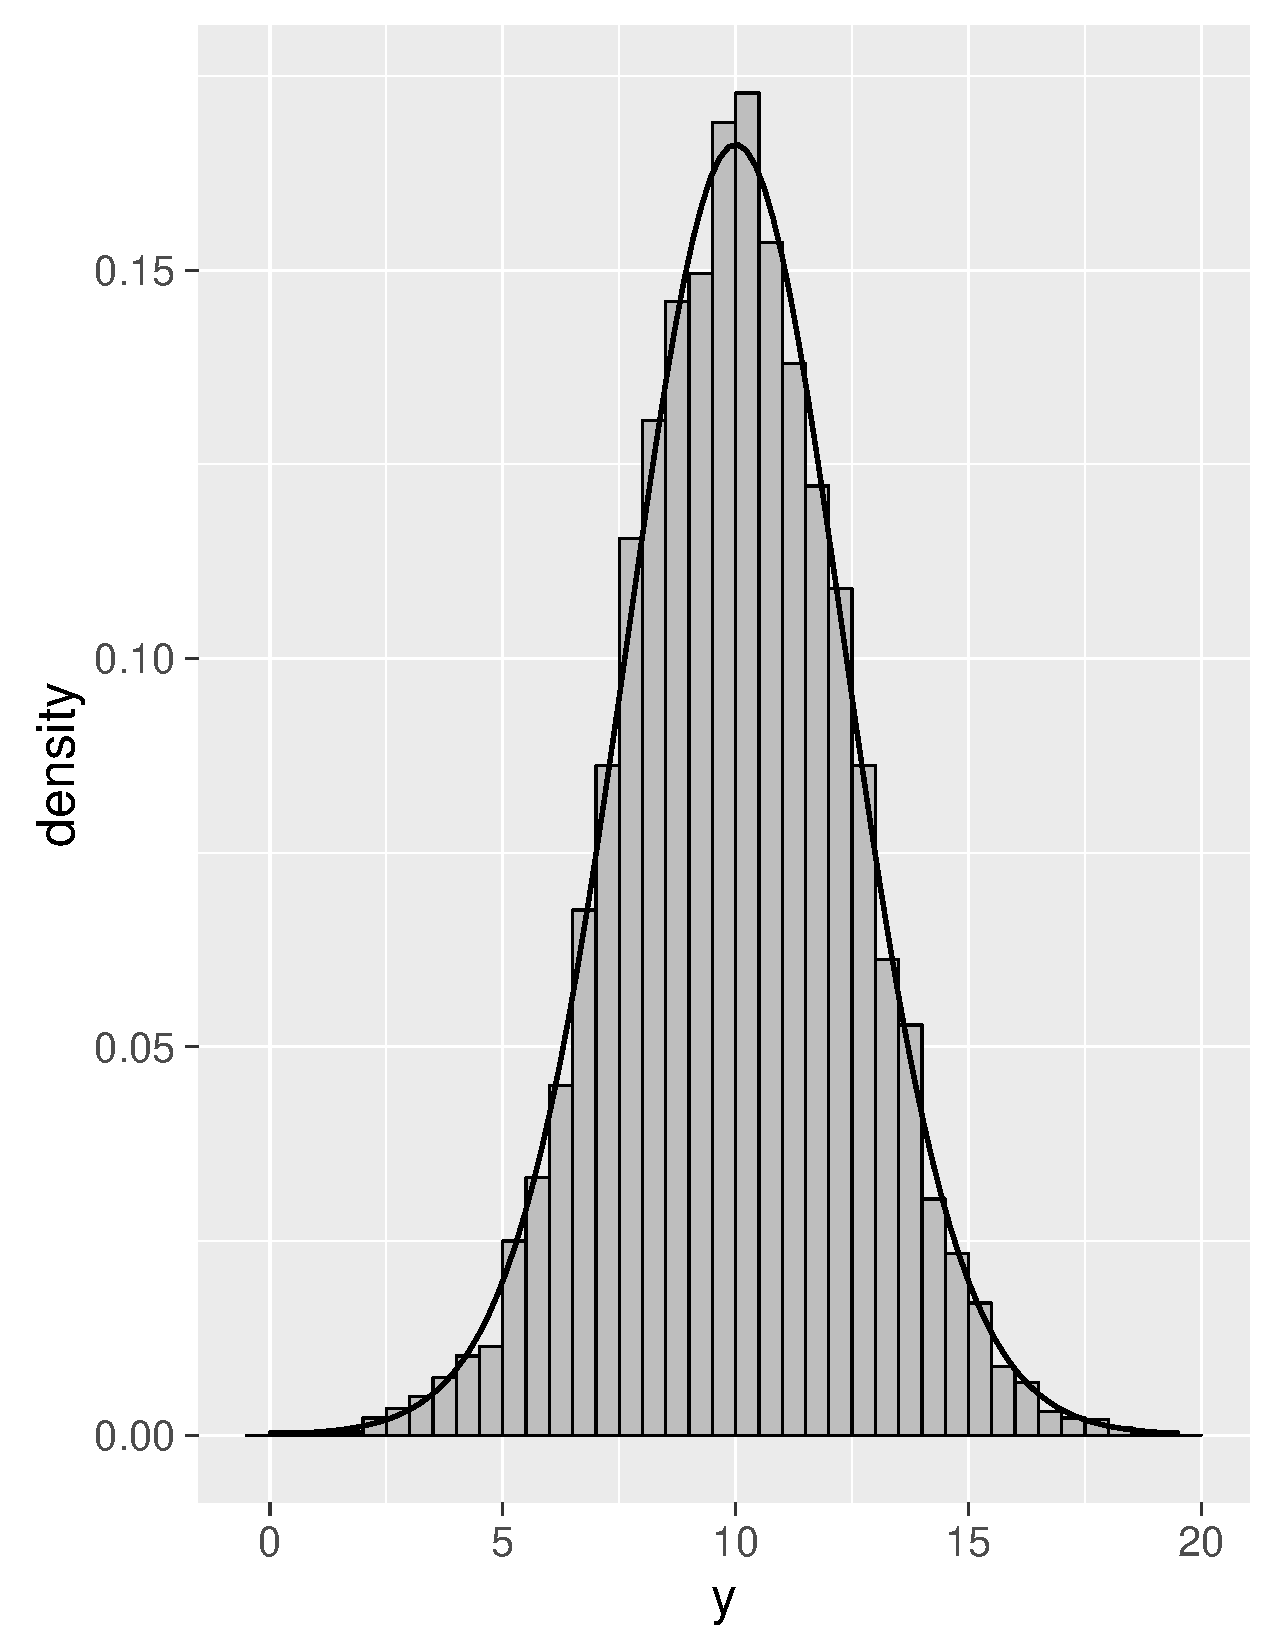
\includegraphics[scale=0.5,width=10cm,height=8cm]{Simu_Y_pred.pdf}
    \caption{\emph{Histograma de 10 mil valores simulados de $\tilde{y}$ y la funci\'on de densidad de la distribuci\'on predictiva $t_{n_0+n}(\theta,\frac{v_0}{n_0+n})$.}}
    \end{figure}
    
    Cuando es de inter\'es conocer el comportamiento de nuevas variables aleatorias $Y_1^*,\cdots,Y_{n^*}^*$, podemos obtener la distribuci\'on predictiva del valor promedio de estas nuevas medicicones: $\bar{Y}^*$. Esta distribuci\'on se encuenta en el siguiente resultado.
    
    \begin{Res}\label{pred_barY_sigma2}
    La distribuci\'on predictiva posterior de la media $\bar{Y}^* $ en una nueva muestrea $Y_1^*,\cdots,Y_{n^*}^*$, cuando se utiliza una distribuci\'on previa informativa para $\sigma^2$, es la distribuci\'on $t$ no estandarizado con grado de libertad $n_0+n$, el par\'ametro de localizaci\'on $\theta$ y el par\'ametro de escala $\frac{v_0}{n^*(n_0+n)}$, donde $v_0=n_0\sigma^2_0+\sum_{i=1}^n(y_i-\theta)^2$, esto es, 
    \begin{equation*}
    \bar{Y}^* \mid \mathbf{Y}\sim t_{n_0+n}\left(\theta,\frac{v_0}{n^*(n_0+n)}\right).
    \end{equation*} 
    
    Cuando se utiliza la distribuci\'on previa no informativa de Jeffreys para $\sigma^2$, la distrubci\'on predictiva de una nueva observaci\'on $\bar{Y}^*$ es
    
    \begin{equation*}
    \bar{Y}^* \mid \mathbf{Y}\sim t_n\left(\theta,\frac{\hat{\sigma}^2_C}{n^*}\right)
    \end{equation*} 
    con $\hat{\sigma}^2_C=\frac{1}{n}\sum_{i=1}^n(y_i-\theta)^2$. 
    \end{Res}
    
    \begin{proof}
    La demostraci\'on del resultado es similar a la del resultado \ref{pred_yy_sigma2}, y se deja como ejercicio para los lectores.
    \end{proof}
    
    \begin{Eje}
    Retomamos los datos usados en el ejemplo \ref{eje_vidrios} donde se cuenta con las siguientes 12 mediciones a l\'aminas de vidrios templados 3.56cm, 3.36cm, 2.99cm, 2.71cm, 3.31cm, 3.68cm, 2.78cm, 2.95cm, 2.82cm, 3.45cm, 3.42cm y 3.15cm. Los resultados inferenciales del ejemplo dejan entrever que el grosor promedio de las l\'aminas de esta l\'inea de producci\'on se puede asumir de 3cm, y queremos conocer un poco acerca de la varianza $\sigma^2$ de esta l\'inea de producci\'on, ya que un valor grande de $\sigma^2$ no es deseable ya que los productos ser\'ia muy "disparejos" entre ellos, y representa una falla para el proceso industrial. 
    
    Al asumir la media conocida $\theta=3cm$, se tiene que la estimaci\'on cl\'asica de $\sigma^2$ viene dada por $\hat{\sigma}^2_C=0.13cm^2$. Al utilizar la distribuci\'on previa no informativa de Jeffreys, la estimaci\'on bayesiana de $\sigma^2$ viene dada por $\frac{n}{n-2}\hat{\sigma}^2_C=0.157cm^2$. Para calcular un intervalo de credibilidad de 95\%, podemos usar el siguiente c\'odigo
\begin{knitrout}
\definecolor{shadecolor}{rgb}{0.933, 0.933, 0.933}\color{fgcolor}\begin{kframe}
\begin{alltt}
\hlkwd{library}\hlstd{(pscl)}
\hlkwd{qigamma}\hlstd{(}\hlnum{0.025}\hlstd{,} \hlkwc{alpha}\hlstd{=}\hlnum{12}\hlopt{/}\hlnum{2}\hlstd{,} \hlkwc{beta}\hlstd{=}\hlnum{12}\hlopt{*}\hlnum{0.13}\hlopt{/}\hlnum{2}\hlstd{)}
\end{alltt}
\begin{verbatim}
## [1] 0.06685
\end{verbatim}
\begin{alltt}
\hlkwd{qigamma}\hlstd{(}\hlnum{0.975}\hlstd{,} \hlkwc{alpha}\hlstd{=}\hlnum{12}\hlopt{/}\hlnum{2}\hlstd{,} \hlkwc{beta}\hlstd{=}\hlnum{12}\hlopt{*}\hlnum{0.13}\hlopt{/}\hlnum{2}\hlstd{)}
\end{alltt}
\begin{verbatim}
## [1] 0.3542
\end{verbatim}
\end{kframe}
\end{knitrout}
    
    de donde el intervalo para $\sigma^2$ est\'a dada por $(0.0668cm^2,0.3542cm^2)$. Para facilitar la interpretaci\'on de la estimaci\'on, es preferible estimar la desviaci\'on est\'andar $\sigma$. La estimaci\'on bayesiana de este par\'ametro ser\'ia $\hat{\sigma}_B=\sqrt{0.157cm^2}\approx 0.4cm$, y un intervalo de credibilidad para $\sigma$ viene dada por $(\sqrt{0.0668cm^2},\sqrt{0.3542cm^2})=(0.25cm,0.59cm)$.
    
    A continuaci\'on se ilustra el uso de \verb'JAGS' para obtener la estimaci\'on bayesiana del par\'ametro $\sigma^2$. En \verb'JAGS' no se admite el comando \verb'dflat()' para especificar una previa no informativa como lo hace \verb'WinBugs', por cual se debe definir la distribuci\'on previa escogiendo los par\'ametros que representa la falta de informaci\'on previa; por otro lado, se acostumbra a usar la distribuci\'on Gamma como la distribuci\'on previa del par\'ametro de precisi\'on $\tau=1/\sigma^2$, tal como se muestra a continuaci\'on.
    
    \colorbox{black}{\textcolor{white}{\textbf{C\'odigo JAGS}}}
\begin{knitrout}
\definecolor{shadecolor}{rgb}{0.933, 0.933, 0.933}\color{fgcolor}\begin{kframe}
\begin{alltt}
\hlstd{IG.model} \hlkwb{<-} \hlkwa{function}\hlstd{()\{}
\hlkwa{for}\hlstd{(i} \hlkwa{in} \hlnum{1} \hlopt{:} \hlstd{n)}
\hlstd{\{}
\hlstd{y[i]} \hlopt{~} \hlkwd{dnorm}\hlstd{(}\hlnum{3}\hlstd{, tau)}
\hlstd{\}}
\hlstd{sigma} \hlkwb{<-} \hlnum{1}\hlopt{/}\hlkwd{sqrt}\hlstd{(tau)}
\hlstd{tau} \hlopt{~} \hlkwd{dgamma}\hlstd{(}\hlnum{0.001}\hlstd{,} \hlnum{0.001}\hlstd{)}
\hlstd{\}}

\hlstd{n} \hlkwb{<-} \hlnum{12}
\hlstd{y} \hlkwb{<-} \hlkwd{c}\hlstd{(}\hlnum{3.56}\hlstd{,} \hlnum{3.36}\hlstd{,} \hlnum{2.99}\hlstd{,} \hlnum{2.71}\hlstd{,} \hlnum{3.31}\hlstd{,} \hlnum{3.68}\hlstd{,} \hlnum{2.78}\hlstd{,} \hlnum{2.95}\hlstd{,} \hlnum{2.82}\hlstd{,} \hlnum{3.45}\hlstd{,} \hlnum{3.42}\hlstd{,} \hlnum{3.15}\hlstd{)}

\hlstd{IG.data} \hlkwb{<-} \hlkwd{list}\hlstd{(}\hlstr{"y"}\hlstd{,}\hlstr{"n"}\hlstd{)}
\hlstd{IG.param} \hlkwb{<-} \hlkwd{c}\hlstd{(}\hlstr{"sigma"}\hlstd{)}
\hlstd{IG.inits} \hlkwb{<-} \hlkwa{function}\hlstd{()\{}
\hlkwd{list}\hlstd{(}\hlstr{"tau"}\hlstd{=}\hlkwd{c}\hlstd{(}\hlnum{1}\hlstd{))}
\hlstd{\}}

\hlstd{IG.fit} \hlkwb{<-} \hlkwd{jags}\hlstd{(}\hlkwc{data}\hlstd{=IG.data,} \hlkwc{inits}\hlstd{=IG.inits, IG.param,} \hlkwc{n.iter}\hlstd{=}\hlnum{10000}\hlstd{,}
\hlkwc{n.burnin}\hlstd{=}\hlnum{1000}\hlstd{,} \hlkwc{model.file}\hlstd{=IG.model)}
\end{alltt}
\begin{verbatim}
## Compiling model graph
##    Resolving undeclared variables
##    Allocating nodes
## Graph information:
##    Observed stochastic nodes: 12
##    Unobserved stochastic nodes: 1
##    Total graph size: 31
## 
## Initializing model
\end{verbatim}
\begin{alltt}
\hlkwd{print}\hlstd{(IG.fit)}
\end{alltt}
\begin{verbatim}
## Inference for Bugs model at "/var/folders/n7/01szs8_x7pq1bvpwwnvq7w_w0000gn/T//RtmpMtD1jH/model11b75fb4487c.txt", fit using jags,
##  3 chains, each with 10000 iterations (first 1000 discarded), n.thin = 9
##  n.sims = 3000 iterations saved
##          mu.vect sd.vect  2.5%   25%    50%    75%  97.5%  Rhat n.eff
## sigma      0.388   0.088 0.261 0.326  0.373  0.434  0.606 1.001  3000
## deviance  10.707   1.486 9.654 9.758 10.126 11.050 15.068 1.001  3000
## 
## For each parameter, n.eff is a crude measure of effective sample size,
## and Rhat is the potential scale reduction factor (at convergence, Rhat=1).
## 
## DIC info (using the rule, pD = var(deviance)/2)
## pD = 1.1 and DIC = 11.8
## DIC is an estimate of expected predictive error (lower deviance is better).
\end{verbatim}
\end{kframe}
\end{knitrout}
    
    Podemos observar que la estimaci\'on bayesiana resultante para $\sigma$ es de 0.387cm, con un intervalo de credibilidad del 95\% de $(0.26cm,0.595cm)$, resultados muy similares a lo presentado anteriormente. 
\end{Eje}

\section{Ejercicios}
\begin{enumerate}
\item\label{XXX} Desarrolla los c\'alculos necesarios para comprobar que para datos normales con varianza conocida, la distribuci\'on posterior de la media $\theta$ es $Normal(\bar{y},\sigma^2/n)$ cuando la distribuci\'on previa es $p(\theta)\propto cte$. 
\item Demuestre el resultado \ref{pred_y_theta}.
\item\label{Ejer_pre_Jeffreys} Demuestre la segunda parte del resultado \ref{pred_norm}.
\item Demuestre que en datos con distribuci\'on normal: $Y_1,\cdots,Y_n\sim N(\theta,\sigma^2)$ con $\theta$ conocido, al utilizar la distribuci\'on previa no informativa de Jeffreys para $\sigma^2$, la distrubci\'on de posterior de $\sigma^2$ viene dada por $Inversa-Gamma(\frac{n}{2},\frac{n\hat{\sigma}^2_C}{2})$ con $\hat{\sigma}^2_C=\frac{1}{n}\sum_{i=1}^n(y_i-\theta)^2$. 
\item\label{pre_y_sigma2_Jeffreys} Demuestre que en datos con distribuci\'on normal: $Y_1,\cdots,Y_n\sim N(\theta,\sigma^2)$ con $\theta$ conocido, al utilizar la distribuci\'on previa no informativa de Jeffreys para $\sigma^2$, la distrubci\'on predictiva de una nueva observaci\'on $\tilde{y}$ es $t_n(\theta,\hat{\sigma}^2_C)$, con $\hat{\sigma}^2_C=\frac{1}{n}\sum_{i=1}^n(y_i-\theta)^2$. 
\item Demuestre el resultado \ref{pred_barY_sigma2}.
\end{enumerate}


